\begin{ex}%[1D9H2-2]
% nguon: Archive/SP_SauLuoi_2024-2025/Sp_GHKII/data/GHKII/1-TN-DS-TLN-TL-THPT-ThiXaQuangTri-QuangTri-GHKII-NH24-25.tex #140
 %[Dự án đề kiểm tra Toán 11 GHKII NH24-25- HectorTran]%[THPT Thị Xã Quảng Trị - Tỉnh Quảng Trị]
	Hai xạ thủ $X$ và $Y$, mỗi người bắn một viên đạn vào một mục tiêu. Xét các biến cố\\
	$A$: \lq\lq Xạ thủ $X$ bắn trúng\rq\rq; $B$: \lq\lq Xạ thủ Y bắn trúng\rq\rq.
	\choiceTF
	{\True Biến cố $A$ và biến cố $B$ độc lập với nhau}
	{\True $AB$ là biến cố \lq\lq Cả hai xạ thủ $X$ và $Y$ bắn trúng\rq\rq}
	{$A\cup B$ là biến cố \lq\lq Có ít hơn một xạ thủ bắn trúng\rq\rq}
	{$\overline{A}B$ là biến cố \lq\lq Xạ thủ $X$ bắn trúng và xạ thủ $Y$ bắn trượt\rq\rq}
	\loigiai{
	 $\overline{A}$: \lq\lq Xạ thủ $X$ bắn trượt\rq\rq, $\overline{B}$: \lq\lq Xạ thủ $Y$ bắn trượt\rq\rq.
		\begin{itemchoice}
			\itemch Do hai xạ thủ $X$ và $Y$, mỗi người bắn một viên đạn vào một mục tiêu nên kết quả bắn của hai xạ thủ là độc lập với nhau. \\ Vậy biến cố $A$ và $B$ độc lập.
			\itemch $AB$ là biến cố cả $A$ và $B$ cùng xảy ra.\\ Do đó, $AB$ là biến cố \lq\lq Cả hai xạ thủ $X$ và $Y$ bắn trúng\rq\rq.
			\itemch $A \cup B$ là biến cố $A$ hoặc $B$ xảy ra.\\
			Do đó $A\cup B$: \lq\lq Có ít nhất một xạ thủ bắn trúng\rq\rq\ ($X$ bắn trúng hoặc $Y$ bắn trúng hoặc cả hai cùng trúng). 
			\itemch $\overline{A}B$ là biến cố $A$ không xảy ra và $B$ xảy ra.\\ Do đó, $\overline{A}B$ là biến cố \lq\lq Xạ thủ $X$ bắn trượt và xạ thủ $Y$ bắn trúng\rq\rq. 
		\end{itemchoice}
	}
\end{ex}

\begin{bt}%[1D9V2-3]
% nguon: Archive/SP_SauLuoi_2024-2025/Sp_GHKII/data/GHKII/1-TN-DS-TLN-TL-THPT-ThiXaQuangTri-QuangTri-GHKII-NH24-25.tex #148
 %[Dự án đề GHKII THPT Thị Xã Quảng Trị - Quảng Trị - 24-25][Lê Phúc]
	Để lên đến đỉnh $S$ của một ngọn núi từ một điểm xuất phát $D$, những người đi bộ có thể đi theo nhiều tuyến đường khác nhau. Hành trình đi không thể kết thúc trong một ngày, vì vậy
	họ phải ngủ lại một đêm ở một trong hai nhà trú ẩn, kí hiệu là $R_1$ và $R_2$. Sáng hôm sau, để lên đến đỉnh núi, họ có hai cách $\colon$ hoặc đi lên đỉnh núi trực tiếp hoặc là đi đến đó sau khi đã dừng nghỉ tại nhà trú ẩn $R_3$. Tình huống được mô tả qua sơ đồ như dưới đây, trong đó khoảng cách
	giữa các điểm (tính bằng km) được cho trên sơ đồ.\\
	Các khảo sát trên một thời gian dài về các tuyến đường đi có thể có cho phép khẳng định rằng
	khi chọn ngẫu nhiên một người đi bộ thì
	\immini{\begin{itemize}
			\item Xác suất mà người này ngủ lại ở nhà trú ẩn $R_1$ là $\dfrac{1}{3}$.\\
			\item Xác suất mà người này leo trực tiếp lên đến đỉnh núi và xuất phát
			từ nhà trú ẩn $R_1$ là $\dfrac{3}{4}$.
			\item Xác suất mà người này leo trực tiếp lên đến đỉnh núi và xuất phát
			từ nhà trú ẩn $R_2$ là $\dfrac{2}{3}$.
		\end{itemize}
		Tính xác suất để anh ta đến đỉnh núi có tổng quảng đường di chuyển lớn hơn $15$ km.} 
	{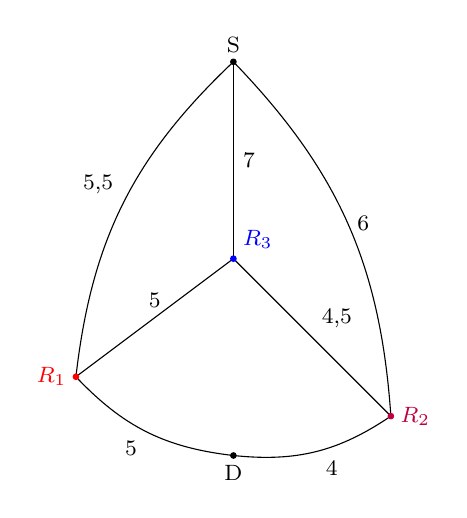
\begin{tikzpicture}[scale=1, font=\footnotesize, line join=round, line cap=round, >=stealth]
			% Các điểm
			\coordinate (D) at (0,0);
			\coordinate (R1) at (-2,1);
			\coordinate (R2) at (2,0.5);
			\coordinate (R3) at (0,2.5);
			\coordinate (S) at (0,5);
			
			% Các đường đi
			\draw (D) to[bend left=20] node[midway, below left] {5} (R1);
			\draw (D) to[bend right=20] node[midway, below right] {4} (R2);
			\draw (R1) to[bend left=20] node[midway, above left] {5,5} (S);
			\draw (R2) to[bend right=20] node[midway, right] {6} (S);
			\draw (R3) to node[midway, right] {7} (S);
			\draw (R1) to node[midway, above] {5} (R3);
			\draw (R2) to node[midway, above right] {4{,}5} (R3);
			
			% Các điểm đánh dấu
			\filldraw[black] (D) circle (1pt) node[below] {D};
			\filldraw[red] (R1) circle (1pt) node[left] {$R_1$};
			\filldraw[purple] (R2) circle (1pt) node[right] {$R_2$};
			\filldraw[blue] (R3) circle (1pt) node[above right] {$R_3$};
			\filldraw[black] (S) circle (1pt) node[above] {S};
	\end{tikzpicture}}
	\loigiai{
		\begin{itemize}
			\item 	Gọi $A$ là biến cố \lq\lq Người này ngủ lại từ nhà trú ẩn $R_1$\rq\rq. \\ $\Rightarrow P(A)=\dfrac{1}{3}$.
			\item 	Gọi $B$ là biến cố \lq\lq Người này ngủ lại từ nhà trú ẩn $R_2$\rq\rq.\\ $\Rightarrow P(B)=\dfrac{2}{3}$.
			\item 	Gọi $C$ là biến cố \lq\lq Người này ở nhà trú ẩn $R_1$ đến $R_3$\rq\rq.\\ $\Rightarrow P(C)=\dfrac{1}{4}$.
			\item 	Gọi $D$ là biến cố \lq\lq Người này ở nhà trú ẩn $R_2$ đến $R_3$\rq\rq.\\ $\Rightarrow P(D)=\dfrac{1}{3}$.
			\item Gọi $K$ là biến cố \lq\lq Người này lên đỉnh núi có tổng quảng đường lớn hơn $15$
			km\rq\rq.
		\end{itemize}
	Để tổng quãng đường lên đỉnh núi lớn hơn $15$ thì người này phải ngủ lại nhà trú ẩn $R_3$.\\
	Do đó người nay đi từ $D$ đến $R_1$ rồi qua $R_3$ và cuối cùng lên đỉnh $S$ \textbf{hoặc} người này đi từ $D$ đến $R_2$ qua $R_3$ và cuối cùng lên đỉnh $S$.\\
	Suy ra $K=AC \cup BD$.\\
	Vì $K=AC \cup BD$ nên 
	\[P(K)=P(A)\cdot P(C)+P(B)\cdot P(K)=\dfrac{1}{3}\cdot\dfrac{1}{4}+\dfrac{2}{3}\cdot\dfrac{1}{3}=\dfrac{11}{36}.\]
	}
\end{bt}

\begin{bt}%[1D9H2-3]
% nguon: Archive/SP_SauLuoi_2024-2025/Sp_GHKII/data/GHKII/1-TN-DS-TLN-TL-THPT-HoaHoi-BRVT-GHKII-NH24-25.tex #162
%[Dự án tex đề GHKII THPT Hoà Hội - Bà Rịa Vũng Tàu- 24-25][Đỗ Minh Vũ]
	 			Một nhóm học sinh có $9$ học sinh nam và $12$ học sinh nữ. Chọn ngẫu nhiên $5$ học sinh từ nhóm học sinh đó. Tính xác suất của biến cố \lq\lq Có $5$ học sinh được chọn đều cùng giới tính\rq\rq.
	 		\loigiai{
	 			Gọi $A$ là biến cố \lq\lq$5$ học sinh được chọn đều là nam\rq\rq $\Rightarrow \mathrm{P}(A)=\dfrac{\mathrm{C}_9^5}{\mathrm{C}_{21} ^5}=\dfrac{2}{323}$;\\
	 			$B$ là biến cố \lq\lq$5$ học sinh được chọn đều là nữ\rq\rq $\Rightarrow \mathrm{P}(B)=\dfrac{\mathrm{C}_{12}^5}{\mathrm{C}_{21}^5}=\dfrac{88}{2261}$;\\
	 			Gọi $X$ là biến cố \lq\lq$5$ học sinh được chọn đều cùng giới tính\rq\rq, ta có $A,B$ là hai biến cố xung khắc nên 
	 			$$\Rightarrow \mathrm{P}(X) = \mathrm{P}(A\cup B) = \mathrm{P}(A)+\mathrm{P}(B) = \dfrac{6}{133}.$$
	 		}
	 	\end{bt}

\begin{bt}%[1D9N1-3]
% nguon: Archive/SP_SauLuoi_2024-2025/Sp_GHKII/data/GHKII/1-TL-TN-DS-THPT-Tran-Quang-Khai-GHKII-NH24-25.tex #186
%[Dự án đề kiểm tra Toán 11 GHKII NH24-25- Phạm Phú]%[THPT Trần Quang Khải - BRVT]
	Lan và Tùng độc lập chơi ném bóng vào rổ. Mỗi bạn ném vào rổ của mình một quả bóng. Biết rằng xác suất ném bóng vào rổ của Lan là $\dfrac{3}{7}$ và của Tùng là $\dfrac{4}{5}$. Xác suất của biến cố "cả hai bạn cùng ném bóng vào rổ" có dạng $P(A)=\dfrac{a}{b}$. Tính giá trị của biểu thức $Q=a+2b$.
		\shortans[]{$82$}
	\loigiai{
	Gọi biến cố A: "Lan ném bóng trúng vào rổ"\\
	Gọi biến cố B: "Tùng ném bóng trúng vào rổ"\\
	Khi đó biến cố AB: "Cả hai bạn cùng ném bóng trúng vào rổ". \\
	Ta có $P(AB)=P(A)\cdot P(B)=\dfrac{3}{7}\cdot \dfrac{4}{5}=\dfrac{12}{35}$. Từ đó $a+2b=12+2\cdot 35=82$.
	}
\end{bt}

\begin{bt}%[1D9N2-3]
% nguon: Archive/SP_SauLuoi_2024-2025/Sp_GHKII/data/GHKII/1-TL-TN-DS-THPT-Tran-Quang-Khai-GHKII-NH24-25.tex #188
%[Dự án đề kiểm tra Toán 11 GHKII NH24-25- Phạm Phú]%[THPT Trần Quang Khải - BRVT]
	Một hộp có $12$ viên bi có cùng kích thướt và khối lượng, trong đó có $7$ viên bi màu xanh và $5$ viên bi màu vàng. Chọn ngẫu nhiên $5$ viên bi từ hộp đó. Tính xác suất để trong $5$ viên  bi được chọn có ít nhất $2$ viên bi vàng.
	\loigiai{
	Ta có không gian mẫu là $n(\Omega)=C_{12}^5=792$.\\
	Gọi biến cố A " Trong 5 viên bi được chọn, có 5 viên bi màu xanh". Khi đó $n(A)=C_7^5=21$.\\
	Gọi biến cố B: " Trong $5$ viên bi được chọn, có $1$ viên bi màu vàng, có $4$ viên bi màu xanh". Khi đó $n(B)=C_5^1\cdot C_7^4=175$.\\
	Xét biến cố M "Trong $5$ viên bi được chọn có ít nhất $2$ viên bi màu vàng"\\
	Khi đó $\overline{M}:$ "trong $5$ viên  bi được chọn có nhiều nhất $1$ viên bi màu vàng"\\
	Ta có $n(\overline{M})=21+175=196$.
	Khi đó $P(\overline{M})=\dfrac{196}{792}=\dfrac{49}{198}$.\\ Suy ra $P(M)=1-P(\overline{M})=1-\dfrac{49}{198}=\dfrac{149}{198}$
	}
\end{bt}

\begin{bt}%[1D9V2-5]
% nguon: Archive/SP_SauLuoi_2024-2025/Sp_GHKII/data/GHKII/1-TN-DS-TLN-TL-THPT-HauNghia-LongAn-GHKII-NH24-25.tex #213
%[Dự án đề kiểm tra Toán 11 GHKII NH24-25 - Đợt 9 - Huỳnh Đức Vũ]%[THPT Hậu Nghĩa - Long An]
Người dân Bình Định truyền nhau câu ca dao
\begin{center}
\lq\lq Muốn ăn bánh ít lá gai\\
Lấy chồng Bình Định sợ dài đường đi.\rq\rq
\end{center}
Muốn ăn bánh ít lá gai thì bạn phải tìm về với xứ Tuy Phước-Bình Định. Nơi đây nổi tiếng trứ danh với món bánh nghe cái tên khá lạ lẫm \lq\lq Bánh ít lá gai\rq\rq\, và hương vị làm say đắm lòng người. Trong một lô sản phẩm trưng bày bánh ít lá gai ở hội chợ ẩm thực huyện Tuy Phước gồm 40 chiếc bánh, $25$ chiếc bánh có nhiều hạt mè và $15$ chiếc bánh có ít hạt mè, một du khách chọn ngẫu nhiên $5$ chiếc bánh. Tính xác suất để du khách đó chọn được ít nhất $2$ chiếc bánh có nhiều hạt mè (biết rằng các chiếc bánh có khả năng được chọn là như nhau) (kết quả làm tròn đến hàng phần nghìn).
\loigiai{	
Lấy $5$ chiếc bánh bất kỳ. Có $ \mathrm{C}_{40}^5$ cách.\\
Lấy ít nhất 2 chiếc bánh có nhiều hạt mè. Có 
$\mathrm{C}_{25}^2\cdot\mathrm{C}_{15}^3+\mathrm{C}_{25}^3\cdot\mathrm{C}_{15}^2+\mathrm{C}_{25}^4\cdot\mathrm{C}_{15}^1+\mathrm{C}_{25}^5$ cách.\\
Xác suất để du khách đó chọn được ít nhất 2 chiếc bánh có nhiều hạt mè\\
$$\dfrac{\mathrm{C}_{25}^2\cdot\mathrm{C}_{15}^3+\mathrm{C}_{25}^3\cdot\mathrm{C}_{15}^2+\mathrm{C}_{25}^4\cdot\mathrm{C}_{15}^1+\mathrm{C}_{25}^5}{\mathrm{C}_{40}^5}\approx 0{,}944.$$}
\end{bt}

\begin{bt}%[1D9V2-4]
% nguon: Archive/SP_SauLuoi_2024-2025/Sp_GHKII/data/GHKII/1-TN-DS-TLN-TL-THPT-NinhBinh-BacLieu-GHKII-NH24-25.tex #227
%[Dự án đề kiểm tra Toán 11 GHKII NH24-25-Lê Minh Thiện Anh]%[THPT Ninh Bình-Bạc Liêu]
	Một nhóm $50$ bệnh nhân có $32$ người điều trị bệnh X, có $18$ người điều trị cả bệnh X và bệnh Y, có $40$ người điều trị ít nhất một trong hai bệnh X hoặc Y. Chọn ngẫu nhiên một bệnh nhân. Xác suất để người đó điều trị bệnh Y và không điều trị bệnh X là $\dfrac{a}{b}$ ($a$, $b$ là các số tự nhiên và nguyên tố cùng nhau). Giá trị của $ab$ bằng bao nhiêu?
	
	\shortans[oly]{100}
	\loigiai{
		Gọi biến cố $A$: \lq\lq Người đó điều trị bệnh X\rq\rq. \\		
		Biến cố $B$: \lq\lq Người đó điều trị bệnh Y\rq\rq. \\		
		Biến cố $A \cup B$: \lq\lq Người đó điều trị ít nhất một trong hai bệnh X hoặc Y\rq\rq. \\		
		Biến cố $\overline{A}B$: \lq\lq Người đó điều trị bệnh Y và không điều trị bệnh X\rq\rq.\\
		Ta có $P(A \cup B) = P(A) + P(B) - P(AB)$ nên \\
		$P(B) = P(A \cup B) - P(A) + P(AB) = \dfrac{40}{50} - \dfrac{32}{50} + \dfrac{18}{30} = \dfrac{13}{25}$. \\
		Ta có $B = AB \cup \overline{A} B$, suy ra $P(B) = P(AB) + P(\overline{A} B)$.\\
		$\Rightarrow P(\overline{A} B) = P(B) - P(AB) = \dfrac{13}{25} - \dfrac{18}{50} = \dfrac{4}{25}$.\\		
		Vậy $\dfrac{a}{b} = \dfrac{4}{25}$. Suy ra $ab=100$.
	}
\end{bt}

\begin{bt}%[1D9H2-4]
% nguon: Archive/SP_SauLuoi_2024-2025/Sp_GHKII/data/GHKII/1-TN-DS-TLN-TL-THPT-Edison-HaiPhong-GKII-NH24-25.tex #257
%[Dự án đề kiểm tra Toán 10 GHKII NH24-25- Quan Ón]%[THPT Edison - Hải Phòng]
	Nhà trường muốn chọn một đội văn nghệ có đủ cả nam và nữ gồm $12$ em đi biểu diễn từ một nhóm học sinh gồm $10$ nam sinh và $8$ nữ sinh. Xác xuất để đội văn nghệ được chọn có đúng $6$ bạn nam là $\dfrac{a}{b}$ $(a\in \mathbb{N}, b \in \mathbb{N})$; $\dfrac{a}{b}$ là phân số tối giản. Tính $a + b$.
	\shortans{291}
	\loigiai{
		Gọi $A$ là biến cố: \lq\lq Đội văn nghệ được chọn có đúng $6$ bạn nam\rq\rq.\\
		Số cách chọn $12$ học sinh bất kỳ (có cả nam và nữ) từ $18$ học sinh là $\mathrm{C}_{18}^{12} = 18\,564$ cách.\\
		Do đó $n(\Omega) = 18\,564$.\\
		Số cách chọn $12$ học sinh trong đó có đúng $6$ bạn nam là $\mathrm{C}_{10}^{6}\cdot\mathrm{C}_{8}^{6} = 5\,880$ cách.\\
		Do đó $n(A) = 5\,880$.\\
		Xác suất để đội văn nghệ được chọn có đúng $6$ bạn nam là
		$$ \mathrm{P}(A) = \dfrac{n(A)}{n(\Omega)} = \dfrac{5\,880}{18\,564} = \dfrac{70}{221}. $$
		Suy ra $a = 70$ và $b = 221 \Rightarrow a + b = 70 + 221 = 291$.
	}
\end{bt}

\begin{bt}%[1D9H1-3]
% nguon: Archive/SP_SauLuoi_2024-2025/Sp_GHKII/data/GHKII/1-TN-DS-TLN-TL-THPT-Edison-HaiPhong-GKII-NH24-25.tex #261
%[Dự án đề kiểm tra Toán 10 GHKII NH24-25- Quan Ón]%[THPT Edison - Hải Phòng]
	Ba người xạ thủ $A_1$, $A_2$, $A_3$ độc lập với nhau cùng nổ súng bắn vào mục tiêu. Biết rằng xác suất bắn trúng mục tiêu của $A_1$, $A_2$, $A_3$ tương ứng là $0{,}7$, $0{,}6$ và $0{,}5$. Tính xác suất để có ít nhất một xạ thủ bắn trúng.
	\loigiai{
		Gọi 
		\begin{itemize}
			\item $A$ là biến cố: \lq\lq Xạ thủ $A_1$ bắn trúng mục tiêu\rq\rq;
			\item $B$ là biến cố: \lq\lq Xạ thủ $A_2$ bắn trúng mục tiêu\rq\rq;
			\item $C$ là biến cố: \lq\lq Xạ thủ $A_3$ bắn trúng mục tiêu\rq\rq.
		\end{itemize}
		Khi đó $A$, $B$, $C$ độc lập và $\mathrm{P}(A) = 0{,}7$; $\mathrm{P}(B) = 0{,}6$; $\mathrm{P}(C) = 0{,}5$.\\
		Xác suất cả ba xạ thủ $A_1$, $A_2$, $A_3$ đều không bắn trúng mục tiêu là 
		$$\mathrm{P}\left(\overline{A}\cdot \overline{B}\cdot \overline{C}\right) = \mathrm{P}\left(\overline{A}\right)\cdot \mathrm{P}\left(\overline{B}\right)\cdot \mathrm{P}\left(\overline{C}\right) = (1 - 0{,}7)\cdot (1 - 0{,}6)\cdot (1 - 0{,}5) = 0{,}06. $$
		Suy ra, xác suất để có ít nhất một xạ thủ bắn trúng mục tiêu là
		$$ 1 - \mathrm{P}\left(\overline{A}\cdot \overline{B}\cdot \overline{C}\right) = 1 - 0{,}06 = 0{,}94. $$
	}
\end{bt}

\begin{bt}%[1D9H1-3]
% nguon: Archive/2024/TOAN_10_XE/TOAN_10_XE/data4/10D9/DS10-C9-B27.tex #412

	Cho hai biến cố $A$ và $B$ với $\mathrm{P}(A)=0{,}3;\mathrm{P}(B)=0{,}4$ và $\mathrm{P}(AB)=0{,}2$. Hỏi hai biến cố $A$ và $B$ có
	\begin{enumerate}
	\item  Xung khắc không?
	\item Độc lập với nhau không?
	\end{enumerate}
	\loigiai{\begin{enumerate}
\item Vì $\mathrm{P}(AB)=0,2\neq 0$ nên hai biến cố $A$ và $B$ không xung khắc.
\item Ta có $\mathrm{P}(A)\cdot\mathrm{P}(B)=0,12\neq 0,2=\mathrm{P}(AB)$ nên hai biến cố $A$ và $B$ không độc lập với nhau.
		\end{enumerate} }
\end{bt}

\begin{bt}%[1D9H1-3]
% nguon: Archive/2024/TOAN_10_XE/TOAN_10_XE/data4/10D9/DS10-C9-B27.tex #414

	Gieo hai đồng xu $A$ và $B$ một cách độc lập. Đồng xu $A$ chế tạo cân đối. Đồng xu $B$ chế tạo không cân đối nên xác suất xuất hiện mặt sấp gấp $3$ lần xác suất xuất hiện mặt ngửa. Tính xác suất để
	\begin{enumerate}
	\item Khi gieo $2$ đồng xu một lần thì cả hai đều ngửa.
	\item Khi gieo $2$ lần thì $2$ lần cả hai đồng xu đều lật ngửa.
	\end{enumerate}
	\loigiai{
\begin{enumerate}
\item Gọi $X$ là biến cố \lq\lq Đồng xu $A$ xuất hiện mặt ngửa \rq\rq.\\
Gọi $Y$ là biến cố \lq\lq Đồng xu $B$ xuất hiện mặt ngửa \rq\rq.\\
Vì đồng xu $A$ chế tạo cân đối nên $\mathrm{P}(X)=\dfrac{1}{2}$.\\
Theo giả thuyết thì xác suất xuất hiện mặt sấp của đồng xu $B$ gấp 3 lần xác suất xuất hiện mặt ngửa do đó $\mathrm{P}(Y)=\dfrac{1}{4}$.\\
Biến cố cần tính cả hai đồng xu đều xuất hiện mặt ngửa là $XY$. Vì $X$, $Y$ là hai biến cố độc lập nên $\mathrm{P}(XY)=\mathrm{P}(X)\cdot \mathrm{P}(Y)=\dfrac{1}{2}\cdot \dfrac{1}{4}=\dfrac{1}{8}$.
\item Xác suất để trong một lần gieo cả hai đồng xu đều ngửa là $\dfrac{1}{8}$.\\ 
Suy ra xác suất khi gieo hai lần thì cả hai lần hai đồng xu đều ngửa là $\left(\dfrac{1}{8}\right)^2=\dfrac{1}{64}$.
\end{enumerate}}
\end{bt}

\begin{bt}%[1D9H1-3]
% nguon: Archive/2024/TOAN_10_XE/TOAN_10_XE/data4/10D9/DS10-C9-B27.tex #415

	Gieo đồng thời 2 con súc sắc cân đối đồng chất, một con màu đỏ và một con màu xanh. Tính xác suất của các biến cố sau
	\begin{enumerate}
	\item Biến cố $A$ ``Con đỏ xuất hiện mặt $6$ chấm''.
	\item Biến cố $B$ ``Con xanh xuất hiện mặt $6$ chấm''.
	\item Biến cố $C$ ``Ít nhất một con suất hiện mặt $6$ chấm''.
	\item Biến cố $D$ ``Không có con nào xuất hiện mặt $6$ chấm''. 
	\item Biến cố $E$ ``Tổng số chấm xuất hiện trên hai con bằng $8$''.
	\item Biến cố $F$ ``Số chấm suất hiện trên hai con súc sắc hơn kém nhau $2$''.
	\end{enumerate}
	\loigiai{
Không gian mẫu $\Omega=\{(a,b)\colon 1\le a,b\le 6\}$.\\ Trong đó $a$ là số chấm trên con đỏ, $b$ là số chấm trên con xanh. Như vậy không gian mẫu $\Omega$ có $36$ phần tử.
\begin{enumerate}
\item Ta có $\Omega=\{(6,b)\colon 1\le b\le 6\}$.\\ Vậy $\mathrm{P}\left(A\right)=\dfrac{n(A)}{n(\Omega)}=\dfrac{6}{36}=\dfrac{1}{6}$.
\item Hoàn toàn tương tự câu a) có $\mathrm{P}\left(B\right)=\dfrac{n(B)}{n(\Omega)}=\dfrac{6}{36}=\dfrac{1}{6}$.
\item Ta có $A\cup B=\{6,6\}$ nên $\mathrm{P}(A\cup B)=\dfrac{1}{36}$.\\
Do đó $\mathrm{P}(C)=\mathrm{P}(A\cup B)=\mathrm{P}(A)+\mathrm{P}(B)-\mathrm{P}(A\cap B)=\dfrac{1}{6}+\dfrac{1}{6}-\dfrac{1}{36}=\dfrac{11}{36}$.
\item Dễ thấy $D$ chính là biến cố đối của $C$ nên $\mathrm{P}\left(D\right)=1-\mathrm{P}\left(C\right)=1-\dfrac{11}{36}=\dfrac{25}{36}$.
\item Các trường hợp thuận lợi của biến cố $E$\\
$E=\{(2,6), (6,2), (3,5), (5,3), (4,4)\}$.\\
Suy ra $n(E)=5$ nên $\mathrm{P}\left(E\right)=\dfrac{n(E)}{n(\Omega)}=\dfrac{5}{36}$.
\item Ta có
\begin{eqnarray*}
F&=&\{\left(a,b\right)\colon 1\le a,b\leq 6, \left|a-b\right|=2\}\\
&=&\{(1,3), (2,4), (3,5), (4,6), (6,4), (5,3), (4,2), (3,1)\}.
\end{eqnarray*}	
Suy ra $n(F)=8$ nên $\mathrm{P}\left(F\right)=\dfrac{n(F)}{n(\Omega)}=\dfrac{8}{36}=\dfrac{2}{9}$.					
		\end{enumerate}}
\end{bt}

\begin{bt}%[1D9H1-3]
% nguon: Archive/2024/TOAN_10_XE/TOAN_10_XE/data4/10D9/DS10-C9-B27.tex #416

An và Bình học ở hai nơi khác nhau. Xác suất để An và Bình đạt điểm giỏi về môn toán trong kỳ thi cuối năm tương ứng là $0{,}92$ và $0{,}88$.
	\begin{enumerate}
	\item Tính xác suất để cả An và Bình đều đạt điểm giỏi.
	\item Tính xác suất để cả An và Bình đều không đạt điểm giỏi.
	\item Tính xác suất để có ít nhất một trong hai bạn An và Bình đạt điểm giỏi.
	\end{enumerate}
	\loigiai{
\begin{enumerate}
\item Gọi $A$ là biến cố “An đạt điểm giỏi về môn toán”.\\
Gọi $B$ là biến cố “Bình đạt điểm giỏi về môn toán”.\\
Vì hai biến cố độc lập nhau nên $\mathrm{P}(AB)=0,92\cdot 0,88=0,8096$.
\item Xác suất để cả An và Bình đều không đạt điểm giỏi: $\mathrm{P}\left(\overline{A}\overline{B}\right)=0,08\cdot 0,12=0,0096$.
\item Xác suất để có ít nhất một trong hai bạn An và Bình đạt điểm giỏi.\\
$\mathrm{P}(A\cup B)=\mathrm{P}(A)+\mathrm{P}(B)-\mathrm{P}(AB)=0,92+0,88-0,8096=0,9904$.
\end{enumerate}	}
\end{bt}

\begin{bt}%[1D9H1-3]
% nguon: Archive/2024/TOAN_10_XE/TOAN_10_XE/data4/10D9/DS10-C9-B27.tex #427
%[Hồng Trường Sơn]
    Một cầu thủ sút bóng vào cầu môn hai lần. Biết rằng xác suất sút vào cầu môn của cầu thủ đó là $\dfrac{3}{8}$.
    \begin{enumerate}[a)]
        \item Tính xác suất để cầu thủ đó sút hai lần bóng đều vào được cầu môn.
        \item Tính xác suất để cầu thủ đó sút không vào cầu môn (sút hụt) ít nhất một lần.
    \end{enumerate}
\loigiai{
    \begin{enumerate}[a)]
        \item Tính xác suất để cầu thủ đó sút hai lần bóng đều vào được câu môn
            \begin{itemize}
                \item Gọi $A$ là biến cố cầu thủ đó sút một lần bóng vào được cầu môn, ta có $\mathrm{P}(A)=\dfrac{3}{8}$.
                \item Gọi $B$ là biến cố cầu thủ đó sút hai lần bóng vào được cầu môn, ta có $$\mathrm{P}(B)=\mathrm{P}(AA)=\mathrm{P}(A)\cdot \mathrm{P}(A)=\dfrac{3}{8}\cdot \dfrac{3}{8}=\dfrac{9}{64}.$$
            \end{itemize}
        \item Tính xác suất để cầu thủ đó sút không vào cầu môn (sút hụt) ít nhất một lần
            \begin{itemize}
                \item Gọi $C$ là biến cố cầu thủ đó sút không vào cầu môn (sút hụt) ít nhất một lần.
                Khi đó $C$ là biến cố đối của $B$.
                \item $\mathrm{P}(C)=1-\mathrm{P}(B)=1-\dfrac{9}{64}=\dfrac{55}{64}$.
            \end{itemize}
    \end{enumerate}
}
\end{bt}

\begin{bt}%[1D9H1-3]
% nguon: Archive/2024/TOAN_10_XE/TOAN_10_XE/data4/10D9/DS10-C9-B27.tex #428
%[Hồng Trường Sơn]
    Có hai xạ thủ bắn bia. Xác suất xạ thủ thứ nhất bắn trúng bia là $0{,}8$. Xác suất xạ thủ thứ hai bắn trúng bia là $0{,}7$. Tính xác suất để
    \begin{enumerate}[a)]
        \item Cả hai xạ thủ đều bắn trúng bia.
        \item Cả hai xạ thủ đều không bắn trúng bia.
        \item Có ít nhất một xạ thủ bắn trúng bia.
    \end{enumerate}
\loigiai{
    \begin{enumerate}[a)]
        \item Cả hai xạ thủ đều bắn trúng bia
            \begin{itemize}
                \item Gọi $A$ là biến cố \lq\lq xạ thủ thứ nhất bắn trúng bia\rq\rq.\\
                    Gọi $B$ là biến cố \lq\lq xạ thủ thứ hai bắn trúng bia\rq\rq.\\
                    Gọi $C$ là biến cố \lq\lq cả hai xạ thủ bắn trúng bia\rq\rq.\\
                    Khi đó $C=AB$.
                \item Vì hai xạ thủ hoạt động độc lập nên $A$ và $B$ là hai biến cố độc lập.\\
                    Áp dụng quy tắc nhân xác suất hai biến cố độc lập, ta có
                    $$\mathrm{P}(C)=\mathrm{P}(A) \cdot \mathrm{P}(B)=0{,}8\cdot 0{,}7=0{,}56.$$
            \end{itemize}
        \item Cả hai xa thủ đều không bắn trúng bia
            \begin{itemize} 
                \item $\overline{A}$ là biến cố \lq\lq xạ thủ thứ nhất bắn trượt bia\rq\rq $\Rightarrow \mathrm{P}(\overline{A})=0,2$.
                \item $\overline{B}$ là biến cố \lq\lq xạ thủ thứ hai bắn trượt bia\rq\rq $\Rightarrow \mathrm{P}(\overline{B})=0,3$.
                \item Gọi $D$ là biến cố \lq\lq cả hai xạ thủ đều không bắn trúng bia\rq\rq.\\
                $\mathrm{P}(D)=\mathrm{P}(\overline{A})\cdot \mathrm{P}(\overline{B})=0{,}2\cdot 0{,}3=0{,}06$.
            \end{itemize}
        \item Có ít nhất một xa thủ bắn trúng bia
            \begin{itemize} 
                \item Gọi $\overline{D}$ là biến cố \lq\lq cả hai xạ thủ đều không bắn trúng\rq\rq. $\overline{D}$ là biến cố đối của $D$.
                \item Ta có $\mathrm{P}(\overline{D})=1-\mathrm{P}(D)=1-0{,}06=0{,}94$.
            \end{itemize}
    \end{enumerate}
}
\end{bt}

\begin{bt}%[1D9C2-4]
% nguon: Archive/2024/TOAN_10_XE/TOAN_10_XE/data4/10D9/DS10-C9-B27.tex #429
%[Hồng Trường Sơn]
    Có hai hòm đựng thẻ, mỗi hòm đựng $13$ thẻ đánh số từ $1$ đến $13$. Từ mỗi hòm rút ngẫu nhiên một thẻ. Tính xác suất để trong hai thẻ rút ra có ít nhất một thẻ đánh số $9$.
    \loigiai{
        \begin{itemize}
            \item Gọi $A$ là biến cố \lq\lq Trong hai thẻ rút ra có ít nhất một thẻ đánh số $9$\rq\rq;
            \item $H$ là biến cố \lq\lq thẻ rút ra từ hòm thứ nhất không đánh số $9$\rq\rq;
            \item $K$ là biến cố \lq\lq thẻ rút ra từ hòm thứ hai không đánh số $9$\rq\rq.
            \item Khi đó $\overline{A}=H\cdot K$. Ta có $P(H)=\dfrac{12}{13} ; P(K)=\dfrac{12}{13}$.
            \item Vì $H$ và $K$ là hai biến cố độc lập nên $P(\overline{A})=P(H\cdot K)=P(H)\cdot P(K)=\dfrac{144}{169}$.
            \item Do đó $P(A)=1-P(\overline{A})=1-\dfrac{144}{169}=\dfrac{25}{169}$ đây là hợp của các biến cố xung khắc.
        \end{itemize}
    }
\end{bt}

\begin{bt}%[1D9V1-3]
% nguon: Archive/2024/TOAN_10_XE/TOAN_10_XE/data4/10D9/DS10-C9-B27.tex #430
%[Hồng Trường Sơn]
    Một chiếc máy bay có hai động cơ $I$ và $II$ hoạt động độc lập với nhau. Xác suất để động cơ $I$ và  động cơ $II$ hoạt động tốt lần lượt là $0{,}8$; $0{,}7$. Tính xác suất để
\begin{enumerate}[a)]
    \item   Cả hai động cơ đều chạy tốt.
    \item Cả hai động cơ đều chạy không tốt.
\end{enumerate}     
    \loigiai{Gọi $A$, $B$ lần lượt là biến cố \lq\lq động cơ $I$, $II$ hoạt động tốt\rq\rq.
    \begin{enumerate}[a)]
        \item Gọi $C$ là biến cố \lq\lq cả hai động cơ đều chạy tốt\rq\rq.\\
        Ta có $A$ và $B$ là hai biến cố độc lập và $C=A\cdot B$.\\
         Khi đó $ \mathrm{P}(C)=\mathrm{P}(AB)=\mathrm{P}(A)\cdot \mathrm{P}(B)=0{,}8\cdot0{,}7=0{,}56$.
        \item Gọi $D$ là biến cố \lq\lq cả hai động cơ đều không chạy tốt\rq\rq.\\
        Ta có $A$ và $B$ là hai biến cố độc lập nên $\overline A$ và $\overline B$ và $C=\overline A\cdot \overline B$. \\
        Do đó $\mathrm{P}(D)=\mathrm{P}(\overline{A})\cdot \mathrm{P}\left(\overline{B}\right) =(1-0{,}8)(1-0{,}7)=0{,}06$.
    \end{enumerate} 
}
\end{bt}

\begin{bt}%[1D9C1-3]
% nguon: Archive/2024/TOAN_10_XE/TOAN_10_XE/data4/10D9/DS10-C9-B27.tex #431
%[Hồng Trường Sơn]
    Gieo hai con súc sắc. Tính xác suất để
    \begin{enumerate}
        \item Cả hai con súc sắc đều xuất hiện mặt $5$ chấm.
        \item Có đúng một trong hai con súc sắc xuất hiện mặt $5$ chấm.
    \end{enumerate}
    \loigiai{
        \begin{enumerate}
            \item Cả hai con súc sắc đều xuất hiện mặt $5$ chấm.
            \begin{itemize}
                \item Gọi $A$ là biến cố \lq\lq Súc sắc $1$ xuất hiện mặt $5$ chấm\rq\rq.
                \item Gọi $B$ là biến cố \lq\lq Súc sắc $2$ xuất hiện mặt $5$ chấm\rq\rq.
                \item Ta có $A$ và $B$ là hai biến cố độc lập và $P(A)=\dfrac{1}{6}, P(B)=\dfrac{1}{6}$.
                \item Biến cố \lq\lq Cả hai con súc sắc đều xuất hiện mặt $5$ chấm\rq\rq là $A\cdot B$.
                \item Vậy xác suất cần tính là $P(A\cdot B)=P(A)\cdot P(B)=\dfrac{1}{6} \cdot \dfrac{1}{6}=\dfrac{1}{36}$.
            \end{itemize}
            \item Có đúng một trong hai con súc sắc xuất hiện mặt $5$ chấm.
            \begin{itemize}
                \item Gọi $C$ là biến cố \lq\lq Có đúng một trong hai con súc sắc xuất hiện mặt $5$ chấm\rq\rq.
                \item Ta có $C$ là hợp của hai biến cố xung khắc $A\cdot \overline{B}$ và $\overline{A}\cdot B$, tức là $C=A \cdot \overline{B} \cup \overline{A}\cdot B$.
                \item Do đó $P(C)=P(A \cdot \overline{B} \cup \overline{A} \cdot B)=P(A \cdot \overline{B})+P(\overline{A} \cdot B)$.
                \item Ta có $P(\overline{A})=1-P(A)=\dfrac{5}{6}, P(\overline{B})=1-P(B)=\dfrac{5}{6}$.
                \item Vì $A$ và $B$ là hai biến cố độc lập với nhau
                \item Nên $\overline{A}$ và $B$ độc lập với nhau; $A$ và $\overline{B}$ độc lập với nhau.\\ 
                Vậy $P(C)=P(A \overline{B})+P(\overline{A} B)=P(A) P(\overline{B})+P(\overline{A}) P(B)=\dfrac{1}{6} \cdot \dfrac{5}{6}+\dfrac{5}{6} \cdot \dfrac{1}{6}=\dfrac{5}{18}$.
            \end{itemize}
        \end{enumerate}
    }
\end{bt}

\begin{bt}%[1D9C2-3]
% nguon: Archive/2024/TOAN_10_XE/TOAN_10_XE/data4/10D9/DS10-C9-B27.tex #432
%[Hồng Trường Sơn]
    Có hai hộp chứa các quả cầu. Hộp thứ nhất chứa $3$ cầu trắng, $7$ quả cầu đỏ và $15$ quả cầu xanh. Hộp thứ hai chứa $10$ cầu trắng, $6$ quả cầu đỏ và $9$ quả cầu xanh. Từ mỗi hộp lấy ngẫu nhiên ra một quả cầu. Tính xác suất để hai quả lấy ra có màu giống nhau.
    \loigiai{
        \begin{itemize}
            \item Gọi $A$ là biến cố \lq\lq Quả cầu được lấy ra từ hộp thứ nhất là màu trắng\rq\rq, $B$ là biến cố \lq\lq Quả cầu được lấy ra từ hộp thứ hai là màu trắng\rq\rq.
            \item Ta có $P(A)=\dfrac{3}{25}, P(B)=\dfrac{10}{25}$.
            \item Vì $A$ và $B$ là hai biến cố độc lập.
            \item Nên xác suất để hai quả cầu lấy ra đều màu trắng là $$P(A B)=P(A) \cdot P(B)=\dfrac{3}{25} \cdot \dfrac{10}{25}=\dfrac{30}{625}$$
            \item Tương tự, xác suất để hai quả cầu lấy ra đều
            \begin{itemize}
                \item Màu xanh $\dfrac{15}{25} \cdot \dfrac{9}{25}=\dfrac{135}{625}$.
                \item Màu đỏ $\dfrac{7}{25} \cdot \dfrac{6}{25}=\dfrac{42}{625}$.
            \end{itemize}
            \item Theo quy tắc cộng, xác suất để hai quả lấy ra có màu giống nhau là 
            $$\dfrac{30}{625}+\dfrac{135}{625}+\dfrac{42}{625}=\dfrac{207}{625}$$
        \end{itemize}
    }
\end{bt}

\begin{bt}%[1D9C2-3]
% nguon: Archive/2024/TOAN_10_XE/TOAN_10_XE/data4/10D9/DS10-C9-B27.tex #433
%[Hồng Trường Sơn]
    Có hai chiếc hộp chứa bi. Hộp thứ nhất chứa $4$ viên bi đỏ và $3$ viên bi trắng. Hộp thứ hai chứa $2$ viên bi đỏ và $4$ viên bi trắng. Lấy ngẫu nhiên từ mỗi hộp ra $1$ viên bi, tính xác suất để $2$ viên bi được lấy ra có cùng màu.
    \loigiai{
        \begin{itemize}
            \item Gọi $A, B, C, D$ lần lượt là các biến cố \lq\lq Lấy được bi đỏ từ hộp thứ nhất\rq\rq, \lq\lq Lấy được bi đỏ từ hộp thứ hai\rq\rq, \lq\lq Lấy được bi trắng từ hộp thứ nhất\rq\rq, \lq\lq Lấy được bi trắng từ hộp thứ hai\rq\rq.
            \item Khi đó $P(A)=\dfrac{4}{7}, P(B)=\dfrac{2}{6}=\dfrac{1}{3}, P(C)=\dfrac{3}{7}, P(D)=\dfrac{4}{6}=\dfrac{2}{3}$.
            \item Gọi $E, F$ lần lượt là các biến cố \lq\lq Hai viên bi lấy ra cùng màu đỏ\rq\rq, \lq\lq Hai viên bi lấy ra cùng màu trắng\rq\rq.\\ 
            Khi đó $E=A B$ và $F=C D$.
            \item Do $A$ và $B$ và hai biến cố độc lập nên $P(E)=P(A\cdot B)=P(A) \cdot P(B)=\dfrac{4}{21}$.
            \item Do $C$ và $D$ là hai biến cố độc lập nên $P(F)=P(C\cdot D)=P(C) \cdot P(D)=\dfrac{2}{7}$.
            \item Do $E$ và $F$ là hai biến cố xung khắc nên xác suất để lấy được hai viên bi cùng màu là 
            $$P(E \cup F)=P(E)+P(F)=\dfrac{4}{21}+\dfrac{2}{7}=\dfrac{10}{21}.$$
        \end{itemize}
    }
\end{bt}

\begin{bt}%[1D9C2-3]
% nguon: Archive/2024/TOAN_10_XE/TOAN_10_XE/data4/10D9/DS10-C9-B27.tex #434
%[Hồng Trường Sơn]
    Có hai hộp, hộp thứ nhất chứa $3$ bi đỏ, $2$ bi xanh và $5$ bi vàng, hộp thứ hai chứa $2$ bi đỏ, $3$ bi xanh và $2$ bi vàng. Lấy ngẫu nhiên $2$ bi, mỗi hộp một bi. Tính xác suất để trong một lần lấy ra được đúng một bi đỏ.
    \loigiai{
        \begin{itemize}
            \item Gọi $A$ là biến cố \lq\lq Trong một lần lấy ra được đúng một bi đỏ\rq\rq.
            \item $\mathrm{A}_{1}$ là biến cố \lq\lq Lấy được bi đỏ ở hộp thứ nhất\rq\rq.
            \item $\mathrm{A}_{2}$ là biến cố \lq\lq Lấy được bi đỏ ở hộp thứ hai\rq\rq.
            \item Ta có $A=A_{1} \overline{A}_{2} \cup \overline{A}_{1} \mathrm{A}_{2} ; P\left(A_{1}\right)=\dfrac{3}{10}, P\left(\overline{A}_{1}\right)=\dfrac{7}{10}, P\left(A_{2}\right)=\dfrac{2}{7}, P\left(\overline{A}_{2}\right)=\dfrac{5}{7}$.
            \item Suy ra 
            \allowbreak
            \begin{eqnarray*}
                P(A)&=&P\left(A_{1} \overline{A}_{2} \cup \overline{A}_{1} \mathrm{A}_{2}\right) \\
                &=&P\left(A_{1} \overline{A}_{2}\right)+P\left(\overline{A}_{1} \mathrm{A}_{2}\right)\\ 
                &=&P\left(A_{1}\right) P\left(\overline{A}_{2}\right)+P\left(\overline{A}_{1}\right) P\left(A_{2}\right)\\
                &=&\dfrac{3}{10} \cdot \dfrac{5}{7}+\dfrac{7}{10} \cdot \dfrac{2}{7}=\dfrac{29}{70}.
            \end{eqnarray*}
        \end{itemize}
    }
\end{bt}

\begin{bt}%[1D9V1-4]
% nguon: Archive/2024/TOAN_10_XE/TOAN_10_XE/data4/10D9/DS10-C9-OTC.tex #438
 %Câu 9.20
 Dự báo thời tiết trong ba ngày thứ Hai, thứ Ba, thứ Tư của tuần sau cho biết, trong mỗi ngày này, khả năng có mưa và không mưa như nhau.
 \begin{enumerate}
 	\item Vẽ sơ đồ hình cây mô tả không gian mẫu. 
	\item  	Tính xác suất của các biến cố:\\
	 F: ``Trong ba ngày, có đúng một ngày có mưa'';\\
	 G: ``Trong ba ngày, có ít nhất hai ngày không mưa''.
 \end{enumerate}
	\loigiai
	{
\begin{enumerate}
	\item Sơ đồ cây
\begin{center}
			\tikzset{solid node/.style={circle,draw,inner sep=1.2,fill=black},hollow node/.style={circle,draw,inner sep=1.2},}
	\begin{tikzpicture}[font=\footnotesize,scale=0.7]
		\tikzset{
			level 1/.style={level distance=15mm,sibling distance=65mm},
			level 2/.style={level distance=15mm,sibling distance=30mm},
			level 3/.style={level distance=15mm,sibling distance=15mm},
			level 4/.style={level distance=15mm,sibling distance=10mm},
		}
		\node[hollow node,label=above:{}]{}
		child{node(T21)[solid node,label=left:{Nắng}]{}
						child{node(T31)[solid node,label=left:{Nắng}]{}
							child{node(T41)[solid node,label=below:{Nắng}]{}edge from parent node[left]{}}
							child{node(T42)[solid node,label=below:{Mưa}]{}edge from parent node[right]{}}
						}
							child{node(T32)[solid node, label=right:{Mưa}]{}
						child{node(T43)[solid node,label=below:{Nắng}]{}edge from parent node[left]{}}
						child{node(T44)[solid node,label=below:{Mưa}]{}edge from parent node[right]{}}
					}
					}
		child{node(T22)[solid node,label=right:{Mưa}]{}
						child{node(T33)[solid node,label=left:{Nắng}]{}
							child{node(T45)[solid node,label=below:{Nắng}]{}edge from parent node[left]{}}
							child{node(T46)[solid node,label=below:{Mưa}]{}edge from parent node[right]{}}
					}
						child{node(T34)[solid node,label=right:{Mưa}]{}
					child{node(T47)[solid node,label=below:{Nắng}]{}edge from parent node[left]{}}
					child{node(T48)[solid node,label=below:{Mưa}]{}edge from parent node[right]{}}
				}
					};
				\draw[dashed](T21)--(T22)node[midway,above]{Thứ 2} (T31)--(T34)node[midway,above]{Thứ 3} (T41)--(T48)node[midway,above]{Thứ 4};
	\end{tikzpicture}
\end{center}
Khi đó không gian mẫu $\Omega=\left\{\text{NNN,NNM,NMN,NMM, MNN,MNM,MMN,MMM} \right\}$.\\
Khi đó $n(\Omega)=8$
\item Ta có $n(F)=2$ suy ra $P(F)=\dfrac{2}{8}=\dfrac{1}{4}.$\\
$n(G)=4$ suy ra $P(G)=\dfrac{4}{8}=\dfrac{1}{2}.$

\end{enumerate}
	}
\end{bt}

\begin{bt}%[1D9V1-4]
% nguon: Archive/2024/TOAN_10_XE/TOAN_10_XE/data4/10D9/DS10-C9-OTC.tex #439
 %9.21
	Gieo một đồng xu cân đối liên tiếp bốn lần.
	\begin{enumerate}
		\item Vẽ sơ đồ hình cây mô tả không gian mẫu.
		\item Tính xác suất để trong bốn lần gieo đó có hai lần xuất hiện mặt sấp và hai lần xuất hiện mặt ngửa.
	\end{enumerate}
 
	\loigiai
	{
\begin{enumerate}
	\item  Sơ đồ cây
	\begin{center}
			\tikzset{solid node/.style={circle,draw,inner sep=1.2,fill=black},hollow node/.style={circle,draw,inner sep=1.2},}
		\begin{tikzpicture}[font=\footnotesize,scale=0.7]
			\tikzset{
				level 1/.style={level distance=15mm,sibling distance=65mm},
				level 2/.style={level distance=15mm,sibling distance=30mm},
				level 3/.style={level distance=15mm,sibling distance=15mm},
				level 4/.style={level distance=15mm,sibling distance=10mm},
			}
			\node[hollow node,label=above:{}]{}
			child{node(h11)[solid node,label=left:{S}]{}
				child{node(h21)[solid node,label=left:{S}]{}
					child{node(h31)[solid node,label=left:{S}]{}
						child{node(h41)[solid node,label=below:{S}]{}edge from parent node[left]{}}
						child{node[solid node,label=below:{N}]{}edge from parent node[right]{}}
						edge from parent node[right]{}}
					child{node(r3)[solid node,label=right:{N}]{}
						child{node[solid node,label=below:{S}]{}edge from parent node[left]{}}
						child{node[solid node,label=below:{N}]{}edge from parent node[right]{}}
						edge from parent node[right]{}}
					edge from parent node[left]{}
				}
				child{node(l2)[solid node,label=right:{N}]{}
					child{node(r3)[solid node,label=left:{S}]{}
						child{node[solid node,label=below:{S}]{}edge from parent node[left]{}}
						child{node[solid node,label=below:{N}]{}edge from parent node[right]{}}
						edge from parent node[right]{}}
					child{node(r3)[solid node,label=right:{N}]{}
						child{node[solid node,label=below:{S}]{}edge from parent node[left]{}}
						child{node[solid node,label=below:{N}]{}edge from parent node[right]{}}
						edge from parent node[right]{}}
					edge from parent node[right]{}
				}
				edge from parent node[left,xshift=-10]{}
			}
			child{node(h12)[solid node,label=right:{N}]{}
				child{node(l1)[solid node,label=left:{S}]{}
					child{node(r3)[solid node,label=left:{S}]{}
						child{node[solid node,label=below:{S}]{}edge from parent node[left]{}}
						child{node[solid node,label=below:{N}]{}edge from parent node[right]{}}
						edge from parent node[right]{}}
					child{node(r3)[solid node,label=right:{N}]{}
						child{node[solid node,label=below:{S}]{}edge from parent node[left]{}}
						child{node[solid node,label=below:{N}]{}edge from parent node[right]{}}
						edge from parent node[right]{}}
					edge from parent node[left]{}
				}
				child{node(h22)[solid node,label=right:{N}]{}
					child{node(r3)[solid node,label=left:{S}]{}
						child{node[solid node,label=below:{S}]{}edge from parent node[left]{}}
						child{node[solid node,label=below:{N}]{}edge from parent node[right]{}}
						edge from parent node[right]{}}
					child{node(h32)[solid node,label=right:{N}]{}
						child{node[solid node,label=below:{S}]{}edge from parent node[left]{}}
						child{node(h42)[solid node,label=below:{N}]{}edge from parent node[right]{}}
						edge from parent node[right]{}}
					edge from parent node[right]{}
				}
				edge from parent node[left,xshift=-10]{}};
					\draw[dashed](h11)--(h12) node[midway,above]{\scriptsize Lần 1} (h21)--(h22) node[midway,above]{\scriptsize Lần 2} (h31)--(h32) node[midway,above]{ \scriptsize Lần 3}  (h41)--(h42) node[midway,above]{\scriptsize Lần 4};
		\end{tikzpicture}
	\end{center}
Không gian mẫu\\
$ \Omega=\left\{\right.  SSSS,SSSN,SSNS,SSNN,
	SNSS,SNSN,SNNS,SNNN, NSSS, NSSN$,\\ $NSNS, NSNN, NNSS,NNSN, NNNS,NNNN \left. \right\}$.\\
Khi đó $n(\Omega)=16.$
\item Gọi $A$ là biến cố ``Trong bốn lần gieo đó có hai lần xuất hiện mặt sấp và hai lần xuất hiện mặt ngửa.''\\
Khi đó $n(A)=5$ suy ra $P(A)=\dfrac{5}{16}.$
\end{enumerate}
	}
\end{bt}

\begin{ex}%[1D9H1-3]
% nguon: Archive/2024/Update-SP-BG10-11-3/SP-3/BG11-3/data_1C5/DeOT-ChuongV-DeOnTap-So2-BuiManhTien.tex #1426
%[24-25- Bài Giảng K10-K11, Bùi Mạnh Tiến]
	Một trường học có tỉ lệ học sinh thích bóng đá là $50\%$, thích bóng rổ là $70\%$ và thích cả hai môn này là $40\%$.
	\choiceTF[t]
	{\True Xác suất để gặp một học sinh trong trường mà em đó thích cả bóng đá và bóng rổ là $0{,}4$}
	{Số học sinh trong trường thích bóng đá nhiều hơn số học sinh thích bóng rổ}
	{Xác suất để gặp một học sinh trong trường mà em đó thích bóng đá và không thích bóng rổ là $0{,}2$}
	{Xác suất để gặp một học sinh trong trường mà học sinh đó không thích bóng đá hoặc không thích bóng rổ là $0{,}7$}
	\loigiai{
		Gọi $A$ là biến cố \lq\lq gặp được một học sinh trong trường thích bóng đá\rq\rq.
		Gọi $B$ là biến cố \lq\lq gặp được một học sinh trong trường thích bóng rổ\rq\rq.
		Khi đó ta có $\mathrm{P}(A)=0{,}5$; $\mathrm{P}(B)=0{,}7$; $P(AB)=0{,}4$.
		\begin{itemchoice}
			\itemch Xác suất để gặp một học sinh trong trường mà em đó thích cả bóng đá và bóng rổ là $0{,}4$.
			\itemch Vì $\mathrm{P}(A)<\mathrm{P}(B)$ nên số học sinh trong trường thích bóng rổ nhiều hơn là bóng đá.
			\itemch Xác suất để một học sinh trong trường đó thích bóng đá mà không thích bóng rổ là
			\begin{align*}
				\mathrm{P}(A)-\mathrm{P}(AB)=0{,}5-0{,}4=0{,}1.
			\end{align*}
			\itemch Xác suất để gặp một học sinh trong trường mà học sinh đó không thích bóng đá hoặc không thích bóng rổ là $1-\mathrm{P}(AB)=1-0{,}4=0{,}6$.
		\end{itemchoice}
	}
\end{ex}

\begin{ex}%[1D9H2-4]
% nguon: Archive/2024/Update-SP-BG10-11-3/SP-3/BG11-3/data_1C5/DeOT-ChuongV-DeOnTap-So2-BuiManhTien.tex #1427
%[24-25- Bài Giảng K10-K11, Bùi Mạnh Tiến]
	Một nhóm học có $100$ học sinh, trong đó có $40$ học sinh giỏi Ngoại ngữ; $30$ học sinh giỏi Tin học và $20$ học sinh giỏi cả ngoại ngữ và tin học. Học sinh nào giỏi ít nhất một trong hai môn sẽ được nhận phần thưởng trong sơ kết học kì. Chọn ngẫu nhiên một trong số $100$ học sinh nói trên. Gọi $A$ là biến cố \lq\lq học sinh được chọn học giỏi Ngoại ngữ\rq\rq, $B$ là biến cố \lq\lq học sinh được chọn học giỏi Tin học\rq\rq, $C$ là biến cố \lq\lq học sinh được chọn được nhận thưởng\rq\rq.
	\choiceTF[t]
	{\True $C=A\cup B$}
	{$\mathrm{P}(C)=\mathrm{P}(A)+\mathrm{P}(B)$}
	{$\mathrm{P}(A)=\dfrac{2}{5}$; $\mathrm{P}(B)=\dfrac{3}{5}$}
	{\True $P(C)=\dfrac{1}{2}$}	
	\loigiai{
		\begin{itemchoice}
			\itemch Vì $C$ là biến cố \lq\lq học sinh được chọn được nhận thưởng\rq\rq $\Leftrightarrow$ \lq\lq học sinh được chọn giỏi ít nhất một trong hai môn Ngoại ngữ hoặc Tin học\rq\rq$\Rightarrow C=A\cup B$.
			\itemch Vì $A$, $B$ không phải hai biến cố xung khắc nên $\mathrm{P}(C)=\mathrm{P}(A\cup B)=\mathrm{P}(A)+\mathrm{P}(B)-\mathrm{P}(AB)$.
			\itemch $n(\Omega)=100$, $n(A)=40\Rightarrow \mathrm{P}(A)=\dfrac{n(A)}{n(\Omega)}=\dfrac{40}{100}=\dfrac{2}{5}$.\\
			$n(B)=30\Rightarrow \mathrm{P}(B)=\dfrac{30}{100}=\dfrac{3}{10}$.
			\itemch $AB$ là biến cố \lq\lq học sinh được chọn giỏi cả Ngoại ngữ và Tin học\rq\rq.\\
			Suy ra $n(AB)=20\Rightarrow \mathrm{P}(AB)=\dfrac{1}{5}$.\\
			$\Rightarrow \mathrm{P}(C)=P(A\cup B)=\mathrm{P}(A)+\mathrm{P}(B)-\mathrm{P}(AB)=\dfrac{2}{5}+\dfrac{3}{10}-\dfrac{1}{5}=\dfrac{1}{2}$.
		\end{itemchoice}
	}
\end{ex}

\begin{bt}%[1D9V2-3]
% nguon: Archive/2024/Update-SP-BG10-11-3/SP-3/BG11-3/data_1C5/DeOT-ChuongV-DeOnTap-So2-BuiManhTien.tex #1432
%[Mức ]%[24-25- Bài Giảng K10-K11, Bùi Mạnh Tiến]
	Hai người $A$ và $B$ cùng nhau chơi một trận đấu tennis diễn ra tối đa $5$ sét đấu. Người nào thắng $3$ sét trước sẽ thắng trận đấu. Biết xác suất giành chiến thắng mỗi sét của $A$ là $0{,}4$. Tính xác suất để $A$ là người thắng trận thi đấu tennis này (kết quả làm tròn đến hàng phần trăm).
	\shortans{$0{,}32$}
	\loigiai{
		Để $A$ thắng chung cuộc thì $A$ phải thắng $3$ trận.
		\begin{itemize}
			\item \textbf{Trường hợp 1}: $A$ và $B$ đấu $3$ trận, khi đó xác suất An thắng trận là $\mathrm{P}_1=(0{,}4)^3=0{,}064$.
			\item \textbf{Trường hợp 2:} $A$ và $B$ đấu $4$ trận, khi đó có $\mathrm{C}_3^1$ cách chọn ra $1$ trận mà $A$ thua ($A$ chỉ có thể thua từ trận thứ nhất đến trận thứ ba vì có $4$ trận đấu). Xác suất để $A$ thắng là $\mathrm{P}_2=\mathrm{C}_3^1\cdot 0{,}6\cdot 0{,}4^3=0{,}1152$.
			\item \textbf{Trường hợp 3:} $A$ và $B$ thi đấu $5$ trận (trận cuối $A$ thắng), khi đó có $\mathrm{C}_4^2$ cách chọn ra $2$ trận mà $A$ thua (từ trận thứ nhất đến trận thứ tư). Xác suất để $A$ thắng là $\mathrm{P}_3=\mathrm{C}_4^2\cdot 0{,}6^2\cdot 0{,}4^3=0{,}13824$.
		\end{itemize} 
		Vậy xác suất để $A$ thắng là $\mathrm{P}_1+\mathrm{P}_2+\mathrm{P}_3=0{,}31744\approx 0{,}32$.
	}
\end{bt}

\begin{bt}%[1D9N2-1]
% nguon: Archive/2024/Update-SP-BG10-11-3/SP-3/BG11-3/data_1C5/Bai-2-Tomtatlythuyet-Dang-1-2-Xacdinhbienco-Quan-On.tex #1464
[Mức 1]%[BG Toán 11 CT2025, Quan Ón]
	Hai xạ thủ X, Y mỗi người bắn một viên đạn vào một mục tiêu. Xét các biến cố\\
	$A$: \lq\lq Xạ thủ X bắn trúng\rq\rq; \\
	$B$: \lq\lq Xạ thủ Y bắn trúng\rq\rq.\\
	Nêu nội dung của các biến cố $AB$, $A\cup B$, $\overline{A}\,\overline{B}$, $\overline{A}B$, $A\overline{B}$, $A\overline{B} \cup \overline{A}B$.
	\loigiai{
		Ta có
		\begin{itemize}
			\item $AB$: \lq\lq Cả hai xạ thủ bắn trúng\rq\rq.
			\item $A\cup B$: \lq\lq Có ít nhất một xạ thủ bắn trúng\rq\rq.
			\item $\overline{A}\,\overline{B}$: \lq\lq Cả hai xạ thủ bắn trượt\rq\rq.
			\item $\overline{A}B$: \lq\lq Xạ thủ X bắn trượt, xạ thủ Y bắn trúng\rq\rq.
			\item $A\overline{B}$: \lq\lq Xạ thủ X bắn trúng, xạ thủ Y bắn trượt\rq\rq.
			\item $A\overline{B} \cup \overline{A}B$: \lq\lq Chỉ có một xạ thủ bắn trúng\rq\rq.
		\end{itemize}
	}
\end{bt}

\begin{bt}%[1D9N2-2]
% nguon: Archive/2024/Update-SP-BG10-11-3/SP-3/BG11-3/data_1C5/Bai-2-Tomtatlythuyet-Dang-1-2-Xacdinhbienco-Quan-On.tex #1465
[Mức 1]
	Một hộp đựng $15$ tấm thẻ cùng loại được đánh số từ $1$ đến $15$. Rút ngẫu nhiên một tấm thẻ trong hộp. Gọi $E$ là biến cố \lq\lq Số ghi trên tấm thẻ là số lẻ\rq\rq; $F$ là biến cố \lq\lq Số ghi trên tấm thẻ là số nguyên tố\rq\rq.
	\begin{enumerate}
		\item Mô tả không gian mẫu.
		\item Nêu nội dung của biến cố hợp $G = E\cup F$. Hỏi $G$ là tập con nào của không gian mẫu?
		\item Nêu nội dung của biến cố giao $H = E\cap F$. Hỏi $H$ là tập con nào của không gian mẫu?
	\end{enumerate}
	\loigiai{
		\begin{enumerate}
			\item Không gian mẫu $\Omega = \{1 ; 2 ; 3 ; 4 ; 5 ; 6 ; 7 ; 8 ; 9 ; 10 ; 11 ; 12 ; 13 ; 14 ; 15\}$.
			\item $G = E\cup F$ là biến cố \lq\lq Số ghi trên tấm thẻ là số lẻ hoặc số nguyên tố\rq\rq.\\
			Ta có $E = \{1 ; 3 ; 5 ; 7 ; 9 ; 11 ; 13 ; 15\}$, $F = \{2 ; 3 ; 5 ; 7 ; 11 ; 13\}$.\\
			Vậy $G = E\cup F = \{1 ; 2 ; 3 ; 5 ; 7 ; 9 ; 11 ; 13 ; 15\}$.
			\item $H = E\cap F$ là biến cố \lq\lq Số ghi trên tấm thẻ vừa là số lẻ vừa là số nguyên tố\rq\rq.\\
			Vậy $H = E\cap F = \left\lbrace 3 ; 5 ; 7 ; 11 ; 13\right\rbrace$.
		\end{enumerate}
	}
\end{bt}

\begin{bt}%[1D9N2-1]
% nguon: Archive/2024/Update-SP-BG10-11-3/SP-3/BG11-3/data_1C5/Bai-2-Tomtatlythuyet-Dang-1-2-Xacdinhbienco-Quan-On.tex #1466
[Mức 1]
	Tung một đồng xu cân đối và đồng chất hai lần liên tiếp. Xét các biến cố\\
	$A$: \lq\lq Đồng xu xuất hiện mặt $S$ ở lần gieo thứ nhất\rq\rq.\\
	$B$: \lq\lq Đồng xu xuất hiện mặt $N$ ở lần gieo thứ nhất\rq\rq.\\
	Hai biến cố trên có xung khắc không?
	\loigiai{
		Ta thấy	$A = \left\lbrace SS; SN\right\rbrace$; $B = \left\lbrace NS; NN\right\rbrace$.\\
		Suy ra $A \cap B = \varnothing$. Do đó, $A$ và $B$ là hai biến cố xung khắc.
	}
\end{bt}

\begin{bt}%[1D9N2-1]
% nguon: Archive/2024/Update-SP-BG10-11-3/SP-3/BG11-3/data_1C5/Bai-2-Tomtatlythuyet-Dang-1-2-Xacdinhbienco-Quan-On.tex #1467
[Mức 1]
	Một hộp có $5$ viên bi xanh, $4$ viên bi đỏ và $2$ viên bi vàng. Lấy ra ngẫu nhiên đồng thời $2$ viên bi từ hộp. Hãy xác định các cặp biến cố xung khắc trong các biến cố sau\\
	$A$: \lq\lq Hai viên bi lấy ra cùng màu xanh\rq\rq;\\
	$B$: \lq\lq Hai viên bi lấy ra cùng màu đỏ\rq\rq;\\
	$C$: \lq\lq Hai viên bi lấy ra cùng màu\rq\rq;\\
	$D$: \lq\lq Hai viên bi lấy ra khác màu\rq\rq.
	\loigiai{
		\begin{enumerate}
			\item Ta có hai biến cố $A$ và $B$ xung khắc.
			\item Biến cố $C$ xảy ra khi lấy ra $2$ viên bi xanh hoặc $2$ viên bi đỏ hoặc $2$ viên bi vàng. Khi lấy được $2$ viên bi màu xanh thì biến cố $A$ và biến cố $C$ cùng xảy ra. Khi lấy được $2$ viên bi màu đỏ thì biến cố $B$ và biến cố $C$ cùng xảy ra. Do đó biến cố $C$ không xung khắc với biến cố $A$ và biến cố $B$.
			\item Biến cố $D$ xảy ra khi lấy ra $1$ viên bi xanh, $1$ viên bi đỏ; hoặc $1$ viên bi xanh, $1$ viên bi vàng; hoặc $1$ viên bi đỏ, $1$ viên bi vàng. Do đó biến cố $D$ xung khắc với biến cố $A$, xung khắc với biến cố $B$ và xung khắc với biến cố $C$.
		\end{enumerate}
		Vậy có $4$ cặp biến cố xung khắc là $A$ và $B$; $A$ và $D$; $B$ và $D$; $C$ và $D$.
	}
\end{bt}

\begin{bt}%[1D9H1-2]
% nguon: Archive/2024/Update-SP-BG10-11-3/SP-3/BG11-3/data_1C5/Bai-2-Tomtatlythuyet-Dang-1-2-Xacdinhbienco-Quan-On.tex #1468
[Mức 2]
	Trong hộp có $1$ quả bóng xanh, $1$ quả bóng đỏ, $1$ quả bóng vàng. Lấy ra ngẫu nhiên $1$ quả bóng, xem màu rồi trả lại hộp. Lặp lại phép thử trên $2$ lần và gọi $A_k$ là biến cố quả bóng lấy ra lần thứ $k$ là bóng xanh $(k = 1, 2)$.
	\begin{enumerate}
		\item $A_1, A_2$ có là các biến cố độc lập không? Tại sao?
		\item Nếu trong mỗi phép thử trên ta không trả bóng lại hộp thì $A_1$, $A_2$ có là các biến cố độc lập không? Tại sao?
	\end{enumerate}
	\loigiai{
		\begin{enumerate}
			\item Nếu $A_1$ xảy ra thì sau khi trả lại quả bóng thứ nhất vào hộp, trong hộp có $1$ quả bóng xanh, $1$ quả bóng đỏ và $1$ quả bóng vàng, do đó xác suất xảy ra $A_2$ là $\dfrac{1}{3}$.\\
			Ngược lại, nếu $A_1$ không xảy ra thì sau khi trả lại quả bóng thứ nhất vào hộp, trong hộp vẫn có $1$ quả bóng xanh, $1$ quả bóng đỏ và $1$ quả bóng vàng, do đó xác suất xảy ra $A_2$ là $\dfrac{1}{3}$.\\
			Ta thấy khi $A_1$ xảy ra hay không xảy ra thì xác suất của biến cố $A_2$ luôn bằng $\dfrac{1}{3}$. Do quả bóng lấy ra lần thứ nhất được trả lại hộp nên biến cố $A_2$ xảy ra hay không xảy ra không ảnh hưởng đến xác suất xảy ra của $A_1$. \\
			Vậy $A_1$ và $A_2$ là hai biến cố độc lập.
			\item Giả sử quả bóng lấy ra lần đầu tiên không được trả lại hộp.\\
			Nếu $A_1$ xảy ra thì trước khi bốc quả bóng thứ hai, trong hộp có $1$ quả bóng đỏ, $1$ quả bóng vàng. Do đó xác suất xảy ra $A_2$ là $0$.\\
			Ngược lại, nếu $A_1$ không xảy ra thì trước khi bốc quả bóng thứ hai, trong hộp có $2$ quả bóng, trong đó có đúng $1$ quả bóng xanh. Do đó xác suất xảy ra $A_2$ là $\dfrac{1}{2}$.\\
			Ta thấy xác suất xảy ra của biến cố $A_2$ phụ thuộc vào sự xảy ra của $A_1$.\\
			Vậy $A_1$ và $A_2$ không là hai biến cố độc lập.
	\end{enumerate}}
\end{bt}

\begin{bt}%[1D9H2-2]
% nguon: Archive/2024/Update-SP-BG10-11-3/SP-3/BG11-3/data_1C5/Bai-2-Tomtatlythuyet-Dang-1-2-Xacdinhbienco-Quan-On.tex #1469
[Mức 2]
	Trong hộp kín có $10$ quả bóng màu xanh và $8$ quả bóng màu đỏ, các quả bóng có kích thước và khối lượng giống nhau. Lấy ngẫu nhiên đồng thời $2$ quả bóng. Xét các biến cố\\
	$A$: \lq\lq Hai quả bóng lấy ra có màu xanh\rq\rq;\\
	$B$: \lq\lq Hai quả bóng lấy ra có màu đỏ\rq\rq.\\
	Chọn phát biểu đúng trong những phát biểu sau đây?
	\begin{enumerate}
		\item Biến cố hợp của hai biến cố $A$ và $B$ là \lq\lq Hai quả bóng lấy ra có cùng màu đỏ hoặc cùng màu xanh\rq\rq;
		\item Biến cố hợp của hai biến cố $A$ và $B$ là \lq\lq Hai quả bóng lấy ra có màu khác nhau\rq\rq;
		\item Biến cố hợp của hai biến cố $A$ và $B$ là \lq\lq Hai quả bóng lấy ra có cùng màu\rq\rq.
	\end{enumerate}
	\loigiai{
		\begin{enumerate}
			\item Phát biểu đúng;
			\item Phát biểu sai;
			\item Phát biểu đúng.
		\end{enumerate}
	}
\end{bt}

\begin{bt}%[1D9N2-1]
% nguon: Archive/2024/Update-SP-BG10-11-3/SP-3/BG11-3/data_1C5/Bai-2-Tomtatlythuyet-Dang-1-2-Xacdinhbienco-Quan-On.tex #1471
[Mức 1]
	Chọn ngẫu nhiên một học sinh trong trường em. Xét hai biến cố sau\\
	$P$: \lq\lq Học sinh đó bị cận thị\rq\rq;\\
	$Q$: \lq\lq Học sinh đó học giỏi môn Toán\rq\rq.\\
	Nêu nội dung của các biến cố $P \cup Q$, $PQ$ và $\overline{P}\,\overline{Q}$.
	\loigiai{
		$P \cup Q$ là biến cố \lq\lq Học sinh đó bị cận thị hoặc học sinh đó giỏi môn Toán\rq\rq.\\
		$PQ$ là biến cố \lq\lq Học sinh đó bị cận thị và học giỏi môn Toán\rq\rq.\\
		$\overline{P}$ là biến cố \lq\lq Học sinh đó không bị cận thị\rq\rq.\\
		$\overline{Q}$ là biến cố \lq\lq Học sinh đó không giỏi môn Toán\rq\rq.\\
		$\overline{P}\,\overline{Q}$ là biến cố \lq\lq Học sinh đó không bị cận và không giỏi môn Toán\rq\rq. 
	}
\end{bt}

\begin{bt}%[1D9N2-1]
% nguon: Archive/2024/Update-SP-BG10-11-3/SP-3/BG11-3/data_1C5/Bai-2-Tomtatlythuyet-Dang-1-2-Xacdinhbienco-Quan-On.tex #1472
[Mức 1]
	Hai vận động viên bắn súng $A$ và $B$ mỗi người bắn một viên vào tấm bia một cách độc lập. Xét các biến  cố sau\\
	$M$: \lq\lq Vận động viên $A$ bắn trúng vòng $10$\rq\rq;\\
	$N$: \lq\lq Vận động viên $B$ bắn trúng vòng $10$\rq\rq.\\
	Hãy biểu diễn các biến cố sau theo biến cố $M$ và $N$.
	\begin{itemize}
		\item $C$: \lq\lq Có ít nhất một vận động viên bắn trúng vòng $10$\rq\rq;
		\item $D$: \lq\lq Cả hai vận động viên bắn trúng vòng $10$\rq\rq;
		\item $E$: \lq\lq Cả hai vận động viên đều không bắn trúng vòng $10$\rq\rq;
		\item $F$: \lq\lq Vận động viên $A$ bắn trúng và vận động viên $B$ không bắn trúng vòng $10$\rq\rq;
		\item  $G$: \lq\lq Chỉ có duy nhất một vận động viên bắn trúng vòng $10$\rq\rq.
	\end{itemize}
	\loigiai{
		\begin{itemize}
			\item $C=A\cup B$;
			\item $D=A\cap B$;
			\item $E=\overline{A}\cap \overline{B}$;\
			\item $F=A\cap \overline{B}$;
			\item $G=A\overline{B}\cup \overline{A}B$.
	\end{itemize}}
\end{bt}

\begin{bt}%[1D9N2-2]
% nguon: Archive/2024/Update-SP-BG10-11-3/SP-3/BG11-3/data_1C5/Bai-2-Tomtatlythuyet-Dang-1-2-Xacdinhbienco-Quan-On.tex #1473
[CD, mức 1]%[TeX hóa Sách 11 CD]%[Hoàng Khắc Ngân]
	Tung một đồng xu cân đối và đồng chất hai lần liên tiếp. Xét các biến cố\\
	$A$: \lq\lq Lần thứ nhất xuất hiện mặt ngửa\rq\rq;\\
	$B$: \lq\lq Lần thứ hai xuất hiện mặt ngửa\rq\rq;\\
	$C$: \lq\lq Cả hai lần đều xuất hiện mặt ngửa\rq\rq;\\
	$D$: \lq\lq Có ít nhất một lần xuất hiện mặt ngửa\rq\rq.\\
	Trong hai biến cố $C, D$, biến cố nào là biến cố hợp của hai biến cố $A$, $B$? Biến cố nào là biến cố giao của hai biến cố $A$, $B$?
	\loigiai{
		Biến cố $C$ là biến cố giao của hai biến cố $A$, $B$.\\
		Biến cố $D$ là biến cố hợp của hai biến cố $A$, $B$.
	}
\end{bt}

\begin{bt}%[1D9N1-2]
% nguon: Archive/2024/Update-SP-BG10-11-3/SP-3/BG11-3/data_1C5/Bai-2-Tomtatlythuyet-Dang-1-2-Xacdinhbienco-Quan-On.tex #1474
[Mức 1]
	Gieo hai con xúc xắc cân đối và đồng chất. Gọi $A$ là biến cố \lq\lq Tổng số chấm xuất hiện trên hai con xúc xắc bằng $5$\rq\rq, $B$ là biến cố \lq\lq Tích số chấm xuất hiện trên hai con xúc xắc bằng $6$\rq\rq.
	\begin{enumerate}
		\item Hãy viết tập hợp mô tả các biến cố trên.
		\item Hãy liệt kê các kết quả của phép thử làm cho cả hai biến cố $A$ và $B$ cùng xảy ra.
	\end{enumerate}
	\loigiai{
		\begin{enumerate}
			\item 	Biến cố $A=\{(1 ; 4) ;(4 ; 1) ;(2 ; 3) ;(3 ; 2)\}$.\\
			Biến cố $B=\{(1 ; 6) ;(6 ; 1) ;(2 ; 3) ;(3 ; 2)\}$.
			\item Kết quả của phép thử làm cho cả hai biến cố $A$ và $B$ cùng xảy ra là $\{(2 ; 3) ;(3 ; 2)\}$.
		\end{enumerate}
	}
\end{bt}

\begin{bt}%[1D9N2-2]
% nguon: Archive/2024/Update-SP-BG10-11-3/SP-3/BG11-3/data_1C5/Bai-2-Tomtatlythuyet-Dang-1-2-Xacdinhbienco-Quan-On.tex #1475
[Mức 1]
	Một hộp đựng $15$ tấm thẻ cùng loại được đánh số từ $1$ đến $15$. Rút ngẫu nhiên một tấm thẻ và quan sát số ghi trên thẻ. Gọi $A$ là biến cố \lq\lq Số ghi trên tấm thẻ nhỏ hơn $7$\rq\rq; $B$ là biến cố \lq\lq Số ghi trên tấm thẻ là số nguyên tố\rq\rq.
	\begin{enumerate}
		\item Mô tả không gian mẫu.
		\item Mỗi biến cố $A \cup B$ và $AB$ là tập con nào của không gian mẫu?
	\end{enumerate}
	\loigiai{
		\begin{enumerate}
			\item Khi rút 1 thẻ từ 15 thẻ được đánh số thì không gian mẫu là: \\
			$\Omega= \{1;2;3;4;5;6;7;8;9;10;11;12;13;14;15 \}$.
			\item 
			Các kết quả thuận lợi của biến cố $A$: $A= \{1;2;3;4;5;6 \}$.\\
			Các kết quả thuận lợi của biến cố $B$: $B=\{2;3;5;7;11;13 \}$.\\
			$A \cup B$ là biến cố \lq\lq Số ghi trên thẻ nhỏ hơn $7$ hoặc số nguyên tố\rq\rq.\\
			$A \cup B = \{1;2;3;4;5;6;7;11;13 \}$.\\
			$AB$ là biến cố \lq\lq Số ghi trên thẻ nhỏ hơn $7$ và nguyên tố\rq\rq.\\
			$AB=\{2;3;5 \}$.
		\end{enumerate}
	}
\end{bt}

\begin{bt}%[1D9N2-2]
% nguon: Archive/2024/Update-SP-BG10-11-3/SP-3/BG11-3/data_1C5/Bai-2-Tomtatlythuyet-Dang-1-2-Xacdinhbienco-Quan-On.tex #1476
[Mức 1]
	Một tổ trong lớp 11B có $4$ học sinh nữ là Hương, Hồng, Dung, Phương và $5$ học sinh nam là Sơn, Tùng, Hoàng, Tiến, Hải. Trong giờ học, giáo viên chọn ngẫu nhiên một học sinh trong tổ đó lên bảng để kiểm tra bài.\\
	Xét các biến cố sau\\
	$H$: \lq\lq Học sinh đó là một bạn nữ\rq\rq;\\
	$K$: \lq\lq Học sinh đó có tên bắt đầu là chữ cái $\mathrm{H}$\rq\rq.
	\begin{enumerate}
		\item Mô tả không gian mẫu.
		\item Nêu nội dung của biến cố hợp $M = H \cup K$. Mỗi biến cố $H$, $K$, $M$ là tập con nào của không gian mẫu?
	\end{enumerate}
	\loigiai{
		\begin{enumerate}
			\item $\Omega=\{\text{Hương, Hồng, Dung, Phương, Sơn, Tùng, Hoàng, Tiến, Hải}\}$.
			\item $M = H\cup K$ là biến cố \lq\lq Học sinh được chọn là một bạn nữ hoặc một bạn nam\rq\rq. \\
			Ta có $H=\{\text{Hương, Hồng, Dung, Phương}\}$;\\
			$K=\{\text{Sơn, Tùng, Hoàng, Tiến, Hải}\}$.\\
			Vậy $M=\Omega=\{\text{Hương, Hồng, Dung, Phương, Sơn, Tùng, Hoàng, Tiến, Hải}\}$.
		\end{enumerate}
	}
\end{bt}

\begin{bt}%[1D9N1-2]
% nguon: Archive/2024/Update-SP-BG10-11-3/SP-3/BG11-3/data_1C5/Bai-2-Tomtatlythuyet-Dang-1-2-Xacdinhbienco-Quan-On.tex #1477
[Mức 1]
	Một tổ trong lớp 11C có $9$ học sinh. Phỏng vấn $9$ bạn này với câu hỏi: \lq\lq Bạn có biết chơi môn thể thao nào trong hai môn này không?\rq\rq. Nếu biết thì đánh dấu X vào ô ghi tên môn thể thao đó, không biết thì để trống. Kết quả thu được như sau
	\begin{center}
		\begin{tabular}{|c|c|c|}
			\hline
			\diagbox{Tên học sinh}{Môn thể thao} & Cầu lông & Bóng bàn \\
			\hline
			Bảo & X & \\
			\hline
			Đăng & X & X \\
			\hline
			Giang & & \\
			\hline
			Hoa & X & X \\
			\hline
			Long & & \\
			\hline
			Mai & X & X \\
			\hline
			Phúc & X & X \\
			\hline
			Tuấn & X & \\
			\hline
			Yến & & \\
			\hline
		\end{tabular}
	\end{center}
	Chọn ngẫu nhiên một học sinh trong tổ. Xét các biến cố sau\\	
	$U$: \lq\lq Học sinh được chọn biết chơi cầu lông\rq\rq;\\
	$V$: \lq\lq Học sinh được chọn biết chơi bóng bàn\rq\rq.
	\begin{enumerate}
		\item Mô tả không gian mẫu.
		\item Nội dung của biến cố giao $T=U \cap V$ là gì? Mối biến cố $U$, $V$, $T$ là tập con nào của không gian mẫu?
	\end{enumerate}
	\loigiai{
		\begin{enumerate}
			\item Không gian mẫu $\Omega=\{\text{Bảo; Đăng; Giang; Hoa; Long; Mai; Phúc; Tuấn; Yến} \}$.
			\item $T$ là biến cố \lq\lq Học sinh được chọn biết chơi cả cầu lông và bóng bàn\rq\rq.\\	
			Ta có: $U=\{\text{Bảo; Đăng; Long; Phúc; Tuấn; Yến}\}$;\\ $V=\{\text{Giang ; Long; Phúc; Tuấn}\}$.\\
			Vậy $T=U \cap V=\{$Long; Phúc; Tuấn$\}$.
		\end{enumerate}
	}
\end{bt}

\begin{bt}%[1D9H2-2]
% nguon: Archive/2024/Update-SP-BG10-11-3/SP-3/BG11-3/data_1C5/Bai-2-Tomtatlythuyet-Dang-1-2-Xacdinhbienco-Quan-On.tex #1478
[Mức 2]
	Một hộp đựng $25$ tấm thẻ cùng loại được đánh số từ $1$ đến $25$. Rút ngẫu nhiên một tấm thẻ trong hộp. Xét các biến cố $P$: \lq\lq Số ghi trên tấm thẻ là số chia hết cho $4$\rq\rq; $Q$: \lq\lq Số ghi trên tấm thẻ là số chia hết cho $6$\rq\rq.
	\begin{enumerate}
		\item Mô tả không gian mẫu.
		\item Nội dung của biến cố giao $S=P Q$ là gì? Mỗi biến cố $P$, $Q$, $S$ là tập con nào của không gian mẫu?
	\end{enumerate} 
	\loigiai{
		\begin{enumerate}
			\item $\Omega=\{1,2,3,4,5,6,7,8,9,10,11,12,13,14,15,16,17,18,19,20,21,22,23,24,25\}$.
			\item $S$ là biến cố \lq\lq Số ghi trên tấm thẻ là số chia hết cho $4$ và chia hết cho $6$\rq\rq.\\	
			Ta có: $P=\{4,8,12,16,20,24\}$; $Q=\{6,12,18,24\}$.\\
			Vậy $S = P\cap Q = \{12;24\}$.
		\end{enumerate} 
	}
\end{bt}

\begin{bt}%[1D9H2-2]
% nguon: Archive/2024/Update-SP-BG10-11-3/SP-3/BG11-3/data_1C5/Bai-2-Tomtatlythuyet-Dang-1-2-Xacdinhbienco-Quan-On.tex #1479
[Mức 2]
	Một hộp có $52$ chiếc thẻ cùng loại, mỗi thẻ được ghi một trong các số $1,2,3, \ldots, 52$; hai thẻ khác nhau thì ghi hai số khác nhau. Rút ngẫu nhiên $1$ chiếc thẻ trong hộp. Xét biến cố $A$: \lq\lq Số xuất hiện trên thẻ được rút ra là số chia hết cho 3\rq\rq \, và biến cố $B$: \lq\lq Số xuất hiện trên thẻ được rút ra là số lẻ\rq\rq. Viết các tập con của không gian mẫu tương ứng với các biến cố $A$, $B$, $A \cap B$.
	\loigiai{
		Ta có $A=\{3 ; 6 ; 9 ; 12 ; 15 ; \ldots ; 48 ; 51\}$;\\
		$B=\{4 ; 8 ; 12 ; 16 ; 20 ; \ldots ; 48 ; 52\}$;\\
		$A \cap B=\{12 ; 24 ; 36 ; 48\}$.
	}
\end{bt}

\begin{bt}%[1D9H2-2]
% nguon: Archive/2024/Update-SP-BG10-11-3/SP-3/BG11-3/data_1C5/Bai-2-Tomtatlythuyet-Dang-1-2-Xacdinhbienco-Quan-On.tex #1480
[Mức 2]
	Gieo hai con xúc xắc cân đối, đồng chất. Xét các biến cố sau:\\
	$E$: \lq\lq Số chấm xuất hiện trên hai con xúc xắc đều là số chẵn\rq\rq;\\
	$F$: \lq\lq Số chấm xuất hiện trên hai con xúc xắc khác tính chẵn lẻ\rq\rq;\\
	$K$: \lq\lq Tích số chấm xuất hiện trên hai con xúc xắc là số chẵn\rq\rq.\\
	Chứng minh rằng $K$ là biến cố hợp của $E$ và $F$.
	\loigiai{
		Để tích của số chấm xuất hiện trên hai con xúc xắc là số chẵn thì có $2$ trường hợp xảy ra.
		\begin{itemize}
			\item TH1: $1$ con xúc xắc xuất hiện mặt chẵn, con còn lại xuất hiện mặt lẻ.\\
			Khi đó số chấm xuất hiện trên hai con xúc xắc khác tính chẵn lẽ.
			\item TH2: $2$ con xúc xắc xuất hiện mặt chẵn.\\
			Do đó $K$ là biến cố hợp của $E$ và $F$.
		\end{itemize}
	}
\end{bt}

\begin{bt}%[1D9H2-1]
% nguon: Archive/2024/Update-SP-BG10-11-3/SP-3/BG11-3/data_1C5/Bai-2-Tomtatlythuyet-Dang-1-2-Xacdinhbienco-Quan-On.tex #1481
[CD, mức 2]%[TeX hóa Sách 11 CD]%[Hoàng Khắc Ngân]
	Gieo ngẫu nhiên một xúc xắc cân đối và đồng chất hai lần liên tiếp. Xét các biến cố\\
	$A$: \lq\lq Số chấm xuất hiện ở lần gieo thứ nhất lớn hơn 4\rq\rq ;\\
	$B$: \lq\lq Số chấm xuất hiện ở lần gieo thứ hai nhỏ hơn 4\rq\rq ;\\
	$C$: \lq\lq Số chấm xuất hiện ở lần gieo thứ nhất nhỏ hơn 4\rq\rq.\\
	Trong các biến cố trên, hãy:
	\begin{enumerate}
		\item Tìm cặp biến cố xung khắc;
		\item Tìm cặp biến cố độc lập.
	\end{enumerate}
	\loigiai{
		\begin{enumerate}
			\item Cặp biến cố xung khắc là $A, C$.
			\item Cặp biến cố độc lập là $A, B$ và $B, C$.
		\end{enumerate}
	}
\end{bt}

\begin{bt}%[1D9H2-1]
% nguon: Archive/2024/Update-SP-BG10-11-3/SP-3/BG11-3/data_1C5/Bai-2-Tomtatlythuyet-Dang-1-2-Xacdinhbienco-Quan-On.tex #1482
[CD, mức 2]%[TeX hóa Sách 11 CD]%[Hoàng Khắc Ngân]
	Một hộp có $3$ quả bóng màu xanh, $4$ quả bóng màu đỏ; các quả bóng có kích thước và khối lượng như nhau. Lấy bóng ngẫu nhiên hai lần liên tiếp, trong đó mỗi lần lấy ngẫu nhiên một quả bóng trong hộp, ghi lại màu của quả bóng lấy ra và bỏ lại quả bóng đó vào hộp.\\
	Xét các biến cố:\\
	$A$: \lq\lq Quả bóng màu xanh được lấy ra ở lần thứ nhất\rq\rq;\\
	$B$: \lq\lq Quả bóng màu đỏ được lấy ra ở lần thứ hai\rq\rq.\\
	Hỏi
	\begin{enumerate}
		\item Hai biến cố $A$ và $B$ có độc lập không? Vì sao?
		\item Hai biến cố $A$ và $B$ có xung khắc không? Vì sao?
	\end{enumerate}
	\loigiai{
		\begin{enumerate}
			\item Trước hết, biến cố $B$ xảy ra sau biến cố $A$ nên việc xảy ra hay không xảy ra của biến cố $B$ không làm ảnh hưởng đến xác suất xảy ra của biến cố $A$.\\
			Mặt khác, ta có xác suất của biến cố $B$ khi biến cố $A$ xảy ra bằng $\dfrac{4}{7}$; xác suất của biến cố $B$ khi biến cố $A$ không xảy ra cũng bằng $\dfrac{4}{7}$.\\
			Do đó việc xảy ra hay không xảy ra của biến cố $A$ không làm ảnh hưởng đến xác suất xảy ra của biến cố $B$.\\
			Vậy hai biến cố $A$ và $B$ là độc lập.
			\item Ta thấy kết quả (xanh; đỏ) là kết quả thuận lợi cho cả hai biến cố $A$ và $B$. Vì thế $A$ và $B$ không là hai biến cố xung khắc.
	\end{enumerate}}		
\end{bt}

\begin{bt}%[1D9H2-1]
% nguon: Archive/2024/Update-SP-BG10-11-3/SP-3/BG11-3/data_1C5/Bai-2-Tomtatlythuyet-Dang-1-2-Xacdinhbienco-Quan-On.tex #1483
[Mức 2]
	Một hộp đựng $4$ viên bi màu đỏ và $5$ viên bi màu xanh, có cùng kích thước và khối lượng.
	\begin{enumerate}
		\item Bạn Minh lấy ngẫu nhiên một viên bi, ghi lại màu của viên bi được lấy ra rồi trả lại viên bi vào hộp. Tiếp theo, bạn Hùng lấy ngẫu nhiên một viên bi từ hộp đó. Xét hai biến cố sau:\\	
		$A$: \lq\lq Minh lấy được viên bi màu đỏ\rq\rq;\\	
		$B$: \lq\lq Hùng lấy được viên bi màu xanh\rq\rq.\\	
		Chứng tỏ rằng hai biến cố $A$ và $B$ độc lập.
		\item Bạn Sơn lấy ngẫu nhiên một viên bi và không trả lại vào hộp. Tiếp theo, bạn Tùng lấy ngẫu nhiên một viên bi từ hộp đó. Xét hai biến cố sau:\\	
		$C$: \lq\lq Sơn lấy được viên bi màu đỏ\rq\rq;\\	
		$D$: \lq\lq Tùng lấy được viên bi màu xanh\rq\rq.\\	
		Chứng tỏ rằng hai biến cố $C$ và $D$ không độc lập.
	\end{enumerate}
	\loigiai{
		\begin{enumerate}
			\item Nếu $A$ xảy ra, tức là Minh lấy được viên bi màu đỏ. Vì Minh trả lại viên bi đã lấy vào hộp nên trong hộp có $4$ viên bi màu đỏ và $5$ viên bi màu xanh. Vậy $P(B)=\dfrac{5}{9}$.\\	
			Nếu $A$ không xảy ra, tức là Minh lấy được viên bi màu xanh. Vì Minh trả lại viên bi đã lấy vào hộp nên trong hộp vẫn có $4$ viên bi màu đỏ và $5$ viên bi màu xanh. Vậy $P(B)=\dfrac{5}{9}$.\\	
			Như vậy, xác suất xảy ra của biến cố $B$ không thay đổi bởi việc xảy ra hay không xảy ra của biến cố $A$.\\	
			Vì Hùng lấy sau Minh nên $P(A)=\dfrac{4}{9}$ dù biến cố $B$ xảy ra hay không xảy ra.\\	
			Vậy $A$ và $B$ độc lập.
			\item Nếu $C$ xảy ra, tức là Sơn lấy được viên bi màu đỏ. Vì Sơn không trả lại viên bi đó vào hộp nên trong hộp có $8$ viên bi với $3$ viên bi màu đỏ và $5$ viên bi màu xanh. Vậy $P(D)=\dfrac{5}{8}$. \\
			Nếu $C$ không xảy ra, tức là Sơn lấy được viên bi màu xanh. Vì Sơn không trả lại viên bi đã lấy vào hộp nên trong hộp có $4$ viên bi màu đỏ và $4$ viên bi màu xanh. Vậy $P(D)=\dfrac{4}{8}$. \\
			Như vậy, xác suất xảy ra của biến cố $D$ đã thay đổi phụ thuộc vào việc biến cố $C$ xảy ra hay không xảy ra. Do đó, hai biến cố $C$ và $D$ không độc lập.
		\end{enumerate}
	}
\end{bt}

\begin{bt}%[1D9H2-1]
% nguon: Archive/2024/Update-SP-BG10-11-3/SP-3/BG11-3/data_1C5/Bai-2-Tomtatlythuyet-Dang-1-2-Xacdinhbienco-Quan-On.tex #1484
[Mức 2]
	Có hai chuồng nuôi thỏ. Chuồng I có $5$ con thỏ đen và $10$ con thỏ trắng. Chuồng II có $3$ con thỏ trắng và $7$ con thỏ đen. Từ mỗi chuồng bắt ngẫu nhiên ra một con thỏ. Xét hai biến cố sau:\\
	$A$: \lq\lq Bắt được con thỏ trắng từ chuồng I\rq\rq;\\
	$B$: \lq\lq Bắt được con thỏ đen từ chuồng Il\rq\rq.\\
	Chứng tỏ rằng hai biến cố $A$ và $B$ độc lập.
	\loigiai{
		Nếu $A$ xảy ra, tức là bắt được con thỏ trắng ở chuồng I. Khi đó, số thỏ ở chuồng II không bị thay đổi và có $3$ thỏ trắng và $7$ thỏ đen. Vậy $P(B)=\dfrac{7}{10}$.\\	
		Nếu $A$ không xảy ra, tức là bắt được thỏ đen ở chuồng I.Khi đó, số thỏ ở chuồng II không bị thay đổi và có $3$ thỏ trắng và $7$ thỏ đen. Vậy $P(B)=\dfrac{7}{10}$.\\	
		Như vậy, xác suất xảy ra của biến cố $B$ không thay đổi bởi việc xảy ra hay không xảy ra của biến cố $A$.\\	
		Tương tự $P(A)=\dfrac{2}{3}$ dù biến cố $B$ xảy ra hay không xảy ra.\\	
		Vậy $A$ và $B$ độc lập.
	}
\end{bt}

\begin{bt}%[1D9H2-1]
% nguon: Archive/2024/Update-SP-BG10-11-3/SP-3/BG11-3/data_1C5/Bai-2-Tomtatlythuyet-Dang-1-2-Xacdinhbienco-Quan-On.tex #1485
[Mức 2]
	Có hai chuồng nuôi gà. Chuồng I có $9$ con gà mái và $3$ con gà trống. Chuồng II có $3$ con gà mái và $6$ con gà trống. Bắt ngẫu nhiên một con gà của chuồng I để đem bán rồi dồn các con gà còn lại của chuồng I vào chuồng II. Sau đó bắt ngẫu nhiên một con gà của chuồng II. Xét hai biến cố sau:\\
	$E$: \lq\lq Bắt được con gà trống từ chuồng I\rq\rq;\\
	$F$: \lq\lq Bắt được con gà mái từ chuồng II\rq\rq.\\
	Chứng tỏ rằng hai biến cố $E$ và $F$ không độc lập.
	\loigiai{
		Nếu $E$ xảy ra, tức là bắt được con gà trống từ chuồng I. Vì con gà trống bị bắt đem đi bán và số gà ở chuồng I dồn vô chuồng II, nên khi bắt gà mái từ chuồng II sẽ có $12$ gà mái và $8$ gà trống. Vậy $P(F)=\dfrac{12}{20}=\dfrac{3}{5}$. \\
		Nếu $E$ không xảy ra, tức là bắt được con gà mái từ chuồng I. Vì con gà mái bị bắt đem đi bán và số gà ở chuồng I dồn vô chuồng II, nên khi bắt gà mái từ chuồng II sẽ có $11$ gà mái và $9$ gà trống. Vậy $P(F)=\dfrac{11}{20}$. \\
		Như vậy, xác suất xảy ra của biến cố $F$ đã thay đổi phụ thuộc vào việc biến cố $E$ xảy ra hay không xảy ra. Do đó, hai biến cố $E$ và $F$ không độc lập.
	}
\end{bt}

\begin{bt}%[1D9H2-5]
% nguon: Archive/2024/Update-SP-BG10-11-3/SP-3/BG11-3/data_1C5/DS11-C5-B2-Dang6-SoDoHinhCay-TranTony.tex #1491
%[Bài giảng 11, Trần Tony]
	Gieo ngẫu nhiên một đồng xu và một con xúc xắc. Sử dụng sơ đồ hình cây mô tả số phần tử của không gian mẫu.
	\loigiai{
		\immini{
			Dựa vào sơ đồ hình cây ta thấy không gian mẫu có $12$ phần tử như sau\\
			$\Omega =\{S1; S2;S3;S4;S5;S6;N1;N2;N3;N4;N5;N6\}$.
		}{
			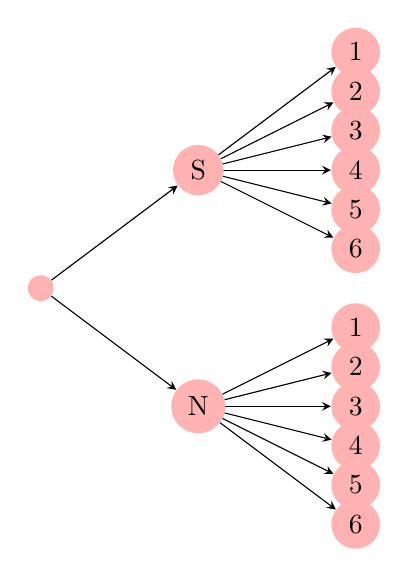
\begin{tikzpicture}[>=stealth,scale=1, line join=round, line cap=round]
				\node[circle, fill=red!30] (a) at (0,0)  {};
				\node[circle, fill=red!30] (b) at (2,1.5)  {\text{S}};
				\node[circle, fill=red!30] (c) at (2,-1.5)  {\text{N}};
				\node[circle, fill=red!30] (d1) at (4,3)  {$1$};
				\node[circle, fill=red!30] (d2) at (4,2.5)  {$2$};
				\node[circle, fill=red!30] (d3) at (4,2)  {$3$};
				\node[circle, fill=red!30] (d4) at (4,1.5)  {$4$};
				\node[circle, fill=red!30] (d5) at (4,1)  {$5$};
				\node[circle, fill=red!30] (d6) at (4,0.5)  {$6$};
				
				\node[circle, fill=red!30] (e1) at (4,-3)  {$6$};
				\node[circle, fill=red!30] (e2) at (4,-2.5)  {$5$};
				\node[circle, fill=red!30] (e3) at (4,-2)  {$4$};
				\node[circle, fill=red!30] (e4) at (4,-1.5)  {$3$};
				\node[circle, fill=red!30] (e5) at (4,-1)  {$2$};
				\node[circle, fill=red!30] (e6) at (4,-0.5)  {$1$};
				\draw[->](a)--(b);\draw[->](a)--(c);
				\draw[->](b)--(d1);\draw[->](b)--(d2);\draw[->](b)--(d3);\draw[->](b)--(d4);\draw[->](b)--(d5);\draw[->](b)--(d6);
				\draw[->](c)--(e1);\draw[->](c)--(e2);\draw[->](c)--(e3);\draw[->](c)--(e4);\draw[->](c)--(e5);\draw[->](c)--(e6);
			\end{tikzpicture}
		}
	}
\end{bt}

\begin{bt}%[1D9H2-5]
% nguon: Archive/2024/Update-SP-BG10-11-3/SP-3/BG11-3/data_1C5/DS11-C5-B2-Dang6-SoDoHinhCay-TranTony.tex #1492
%[Bài giảng 11, Trần Tony]
	Vẽ sơ đồ hình cây để chọn ra $2$ bạn để phân công trực nhật trong một tổ có $4$ nam và $5$ nữ. 
	\loigiai{
		Dựa vào yêu cầu bài toán, ta có sơ đồ hình cây sau:
		\begin{center}
			\begin{tikzpicture}[scale=0.2,>=stealth,every node/.style={shape=rectangle,draw,rounded corners, color=blue, fill=blue!10}]
				%-------------
				\tikzstyle{block} = [rectangle, draw, fill=blue!10, rounded corners, text centered, text width = 9em, minimum height = 1em]
				%-------------
				\node (c1) [block] {Lấy ngẫu nhiên $2$ bạn trong tổ};
				\node (c2) [block, below right = 1.5cm of c1]{Lấy $2$ bạn nam ($\mathrm{C_4^2}$)};
				\node (c3) [block, below= 0.6cm of c1]{Lấy $1$ bạn nam ($\mathrm{C_4^1}$)};
				\node (c4) [block, below left= 1.5cm of c1]{Lấy $2$ bạn nữ ($\mathrm{C_5^2}$)};
				\node (c5) [block,below = 1cm of c2]{Có $6$ cách};
				\node (c6) [block,below = 0.5cm of c3]{Lấy $1$ bạn nữ ($\mathrm{C_5^1}$)};
				\node (c7) [block,below = 1cm of c4]{Có $10$ cách};
				\node (c8) [block,below = 0.5cm of c6]{Có $\mathrm{C_4^1}\cdot\mathrm{C_5^1}$ cách};
				%--------------
				\draw[->] (c1.south) -- (c2.north);
				\draw[->] (c1.south) -- (c3.north);
				\draw[->] (c1.south) -- (c4.north);
				\draw[->] (c2.south) -- (c5.north);
				\draw[->] (c3.south) -- (c6.north);
				\draw[->] (c4.south) -- (c7.north);
				\draw[->] (c6.south) -- (c8.north);
			\end{tikzpicture}
		\end{center}
		Theo sơ đồ hình cây trên thì số phần tử của không gian mẫu của phép thử là\\ $n({\Omega})=10+\mathrm{C_5^1}\cdot\mathrm{C_4^1}+6=36$.
	}
\end{bt}

\begin{bt}%[1D9H2-5]
% nguon: Archive/2024/Update-SP-BG10-11-3/SP-3/BG11-3/data_1C5/DS11-C5-B2-Dang6-SoDoHinhCay-TranTony.tex #1493
%[Bài giảng 11, Trần Tony]
	Một hộp chứa $7$ quả cầu đỏ và $5$ quả cầu xanh. Lấy ngẫu nhiên từ hộp ra $3$ quả cầu, sử dụng sơ đồ hình cây mô tả số phần tử của không gian mẫu của phép thử.
	\loigiai{ Dựa vào yêu cầu bài toán, ta có sơ đồ hình cây sau:
		\begin{center}
			\begin{tikzpicture}[scale=.2,>=stealth,every node/.style={shape=rectangle,draw,rounded corners, color=blue, fill=blue!10}]
				%-------------
				\tikzstyle{block} = [rectangle, draw, fill=blue!10, rounded corners, text centered, text width = 9em, minimum height = 2em]
				%-------------
				\node (c1)[block] {Lấy ngẫu nhiên $3$ quả cầu từ trong hộp};
				\node (tmp) [below = 2cm of c1, inner sep=0, minimum size=0pt] {};
				\node (c2) [block, right = 4.8cm of tmp]{Lấy $3$ quả màu đỏ\\ ($\mathrm{C_7^3}$)};
				\node (c3) [block, left = 4.8cm of tmp]{Lấy $3$ quả màu xanh ($\mathrm{C_5^3}$)};
				\node (c4) [block, left = 0.3cm of c2]{Lấy $2$ quả màu đỏ\\  ($\mathrm{C_7^2}$)};
				\node (c5) [block, right = 0.3cm of c3]{Lấy $2$ quả màu xanh ($\mathrm{C_5^2}$)};
				\node (c6) [block,below =3cm of c2]{Có $35$ cách};
				\node (c7) [block, below = 3cm of c3]{Có $10$ cách};
				\node (c8) [block, below = 1cm of c4]{Lấy $1$ quả màu xanh ($\mathrm{C_5^1}$)};
				\node (c9) [block, below = 1cm of c5]{Lấy $1$ quả màu đỏ \\ ($\mathrm{C_7^1}$)};
				\node (c10) [below = 1cm of c9]{Có $\mathrm{C_7^1}\cdot\mathrm{C_5^2}$ cách};
				\node (c11) [below = 1cm of c8]{Có $\mathrm{C_5^1}\cdot\mathrm{C_7^2}$ cách};
				%--------------
				\draw[->] (c1.south) -- (c2.north);
				\draw[->] (c1.south) -- (c3.north);
				\draw[->] (c1.south) -- (c4.north);
				\draw[->] (c1.south) -- (c5.north);
				\draw[->] (c2.south) -- (c6.north);
				\draw[->] (c3.south) -- (c7.north);
				\draw[->] (c4.south) -- (c8.north);
				\draw[->] (c5.south) -- (c9.north);	
				\draw[->] (c9.south) -- (c10.north);
				\draw[->] (c8.south) -- (c11.north);
			\end{tikzpicture}
		\end{center}
		Theo sơ đồ hình cây trên thì số phần tử của không gian mẫu của phép thử là $$n({\Omega})=10+\mathrm{C_5^1}\cdot\mathrm{C_7^2}+\mathrm{C_5^2}\cdot\mathrm{C_7^1}+35=220.$$
	}
\end{bt}

\begin{bt}%[1D9H2-5]
% nguon: Archive/2024/Update-SP-BG10-11-3/SP-3/BG11-3/data_1C5/DS11-C5-B2-Dang6-SoDoHinhCay-TranTony.tex #1494
%[Bài giảng 11, Trần Tony]
	Một hộp chứa $5$ quả cầu màu xanh và $8$ quả cầu màu đỏ. Lập sơ đồ hình cây của biến cố A "Lấy được $3$ quả cầu và có đủ cả hai màu".
	\loigiai{
		Dựa vào yêu cầu bài toán, ta có sơ đồ hình cây sau:
		\begin{center}
			\begin{tikzpicture}[scale=0.2,>=stealth,every node/.style={shape=rectangle,draw,rounded corners, color=blue, fill=blue!10}]
				%-------------
				\tikzstyle{block} = [rectangle, draw, fill=blue!10, rounded corners, text centered, text width = 10em, minimum height = 2em]
				%-------------
				\node (c1) [block] {Lấy ngẫu nhiên $3$ quả cầu và có đủ cả hai màu};
				\node (c2) [block, below right = 1cm of c1]{Lấy $1$ quả cầu màu đỏ\\ ($\mathrm{C_8^1}$)};
				\node (c3) [block, below left= 1cm of c1]{Lấy $2$ quả cầu màu đỏ\\ ($\mathrm{C_8^2}$)};
				\node (c4) [block,below = 1cm of c2]{Lấy $2$ quả cầu màu xanh\\ ($\mathrm{C_5^2}$)};
				\node (c5) [block,below = 1cm of c3]{Lấy $1$ quả cầu màu xanh\\ ($\mathrm{C_5^1}$)};
				\node (c6) [block,below = 1cm of c4]{Có $\mathrm{C_8^1}\cdot\mathrm{C_5^2}$ cách};
				\node (c7) [block,below = 1cm of c5]{Có $\mathrm{C_8^2}\cdot\mathrm{C_5^1}$ cách};
				%--------------
				\draw[->] (c1.south) -- (c2.north);
				\draw[->] (c1.south) -- (c3.north);
				\draw[->] (c2.south) -- (c4.north);
				\draw[->] (c3.south) -- (c5.north);
				\draw[->] (c4.south) -- (c6.north);
				\draw[->] (c5.south) -- (c7.north);
			\end{tikzpicture}
		\end{center}
		Vậy số phần tử của biến cố A là $n_{(\mathrm{A})}=\mathrm{C_8^1}\cdot\mathrm{C_5^2}+\mathrm{C_8^2}\cdot\mathrm{C_5^1}=220$.
	}
\end{bt}

\begin{bt}%[1D9H2-5]
% nguon: Archive/2024/Update-SP-BG10-11-3/SP-3/BG11-3/data_1C5/DS11-C5-B2-Dang6-SoDoHinhCay-TranTony.tex #1495
%[Bài giảng 11, Trần Tony]
	Trong một ngân hàng đề kiểm tra có ba loại câu hỏi dễ - trung bình - khó. Biết loại dễ có $10$ câu, loại trung bình có $8$ câu và loại khó có $4$ câu. Giáo viên cần tạo ra một đề thi có $3$ câu từ ngân ngàng đề thi đó. Lập sơ đồ hình cây cho biến cố "Đề thi được tạo thành có đúng $2$ loại câu hỏi".
	\loigiai{
		Dựa vào yêu cầu bài toán, ta có sơ đồ hình cây sau:
		\begin{center}
			\begin{tikzpicture}[scale=.2,>=stealth,every node/.style={shape=rectangle,draw,rounded corners, color=blue, fill=blue!10}]
				%-------------
				\tikzstyle{block} = [rectangle, draw, fill=blue!10, rounded corners, text centered, text width = 6em, minimum height = 3em]
				%------------- cấp 1
				\node (c1) [block] {Lấy ngẫu nhiên $3$\\ câu hỏi chỉ thuộc $2$ loại câu hỏi};
				\node (c2) [block, above right = 1cm of c1]{Lấy $1$ câu hỏi dễ\\ có $10$ cách};
				\node (c3) [block, right= 0.7cm of c1]{Lấy $1$ câu hỏi trung bình\\ có $8$ cách};
				\node (c4) [block, below right= 1cm of c1]{Lấy $1$ câu hỏi khó\\ có $4$ cách};
				%--------------- cấp 2
				\node (c5) [block,below right = 3.5cm of c2]{Lấy $2$ câu hỏi trung bình có $\mathrm{C_8^2}$\\cách chọn};
				\node (c6) [block,above right= 3.5cm of c2]{Lấy $2$ câu hỏi khó\\ có $\mathrm{C_4^2}$\\cách chọn};
				\node (c7) [block,below right = 3.5cm of c3]{Lấy $2$ câu hỏi dễ\\ có $\mathrm{C_{10}^2}$\\cách chọn};
				\node (c8) [block,above right= 3.5cm of c3]{Lấy $2$ câu hỏi khó\\ có $\mathrm{C_4^2}$\\cách chọn};
				\node (c9) [block,below right = 3.5cm of c4]{Lấy $2$ câu hỏi trung bình\\ có $\mathrm{C_8^2}$\\cách chọn};
				\node (c10) [block,above right= 3.5cm of c4]{Lấy $2$ câu hỏi dễ\\ có $\mathrm{C_{10}^2}$\\cách chọn};
				%-------------- cấp 3
				\node (c11) [block,right = 0.5cm of c5]{Vậy có $10\cdot\mathrm{C_8^2}$ cách chọn};
				\node (c12) [block,right = 0.5cm of c6]{Vậy có $10\cdot\mathrm{C_4^2}$ cách chọn};
				\node (c13) [block,right = 0.5cm of c7]{Vậy có $8\cdot\mathrm{C_{10}^2}$ cách chọn};
				\node (c14) [block,right = 0.5cm of c8]{Vậy có $8\cdot\mathrm{C_4^2}$ cách chọn};
				\node (c15) [block,right = 0.5cm of c9]{Vậy có $4\cdot\mathrm{C_{8}^2}$ cách chọn};
				\node (c16) [block,right = 0.5cm of c10]{Vậy có $4\cdot\mathrm{C_{10}^2}$ cách chọn};
				%--------------- các đường nối các block
				\draw[->] (c1.east) -- (c2.west);
				\draw[->] (c1.east) -- (c3.west);
				\draw[->] (c1.east) -- (c4.west);
				\draw[->] (c2.east) -- (c5.west);
				\draw[->] (c2.east) -- (c6.west);
				\draw[->] (c3.east) -- (c7.west);
				\draw[->] (c3.east) -- (c8.west);
				\draw[->] (c4.east) -- (c9.west);
				\draw[->] (c4.east) -- (c10.west);
				\draw[->] (c5.east) -- (c11.west);
				\draw[->] (c6.east) -- (c12.west);
				\draw[->] (c7.east) -- (c13.west);
				\draw[->] (c8.east) -- (c14.west);
				\draw[->] (c9.east) -- (c15.west);
				\draw[->] (c10.east) -- (c16.west);
			\end{tikzpicture}
		\end{center}
		Vậy số phần tử của biến cố cần tìm là $10\cdot\mathrm{C_8^2}+10\cdot\mathrm{C_4^2}+8\cdot\mathrm{C_{10}^2}+8\cdot\mathrm{C_4^2}+4\cdot\mathrm{C_{8}^2}+4\cdot\mathrm{C_{10}^2}=1040 $.
	}
\end{bt}

\begin{bt}%[1D9H2-5]
% nguon: Archive/2024/Update-SP-BG10-11-3/SP-3/BG11-3/data_1C5/DS11-C5-B2-Dang6-SoDoHinhCay-TranTony.tex #1496
%[Bài giảng 11, Trần Tony]
	Rút ngẫu nhiên $4$ lá bài từ một bộ bài Tây. Lập sơ đồ hình cây cho biến cố $\mathrm{A}\colon$ "Rút được ít nhất $2$ con Át".
	\loigiai{
		Dựa vào yêu cầu bài toán, ta có sơ đồ hình cây sau:
		\begin{center}
			\begin{tikzpicture}[scale=.3,>=stealth,every node/.style={shape=rectangle,draw,rounded corners, color=blue, fill=blue!10}]
				%-------------
				\tikzstyle{block} = [rectangle, draw, fill=blue!10, rounded corners, text centered, text width = 6em, minimum height = 3em]
				%------------- cấp 1
				\node (c1) [block] {Lấy được ít nhất $2$ quân Át};
				\node (c2) [block, above right = 1cm of c1]{Lấy $2$ quân Át có $\mathrm{C_4^2}$ cách lấy};
				\node (c3) [block, right= 0.7cm of c1]{Lấy $3$ quân Át có $\mathrm{C_4^3}$ cách lấy};
				\node (c4) [block, below right= 1cm of c1]{Lấy $4$ quân Át có $1$ cách lấy};
				%--------------- cấp 2
				\node (c5) [block,right = 1cm of c2]{Lấy $2$ quân bất kỳ còn lại có $\mathrm{C_{48}^2}$ cách lấy};
				\node (c6) [block,right = 1cm of c3]{Lấy $1$ quân bất kỳ còn lại có $\mathrm{C_{48}^1}$ cách lấy};
				\node (c7) [block,right = 4cm of c4]{Có $1$ cách lấy};
				%................ cấp 3
				\node (c8) [block,right = 1cm of c5]{Có $\mathrm{C_4^2}\cdot\mathrm{C_{48}^2}$ cách lấy};
				\node (c9) [block,right = 1cm of c6]{Có $\mathrm{C_4^3}\cdot\mathrm{C_{48}^1}$ cách lấy};
				%--------------- các đường nối các block
				\draw[->] (c1.east) -- (c2.west);
				\draw[->] (c1.east) -- (c3.west);
				\draw[->] (c1.east) -- (c4.west);
				\draw[->] (c2.east) -- (c5.west);
				\draw[->] (c3.east) -- (c6.west);
				\draw[->] (c4.east) -- (c7.west);
				\draw[->] (c5.east) -- (c8.west);
				\draw[->] (c6.east) -- (c9.west);
			\end{tikzpicture}
		\end{center}
		Vậy số phần tử của biến cố cần tìm là\\
		$n{(\mathrm{A})}=1+ \mathrm{C_4^2}\cdot\mathrm{C_{48}^2} + \mathrm{C_4^3}\cdot\mathrm{C_{48}^1}=6961$.
	}
\end{bt}

\begin{bt}%[1D9H2-5]
% nguon: Archive/2024/Update-SP-BG10-11-3/SP-3/BG11-3/data_1C5/DS11-C5-B2-Dang6-SoDoHinhCay-TranTony.tex #1497
%[Bài giảng 11, Trần Tony]
	Câu lạc bộ nghệ thuật của một trường trung học phổ thông gồm học sinh của cả ba khối $10$, $11$, $12$, mỗi khối có $5$ học sinh. Chọn ngẫu nhiên $3$ học sinh để tham gia biểu diễn. Tính xác suất để $3$ học sinh được chọn chỉ thuộc hai khối.
	\loigiai{
	Mỗi cách chọn ra đồng thời $3$ học sinh trong câu lạc bộ cho ta một tổ hợp chập $3$ của $15$ phần tử. Do đó, không gian mẫu $\Omega$ gồm các tổ hợp chập $3$ của $15$ phần tử và
	$$
	n(\Omega)=\mathrm{C}_{15}^3=\dfrac{15!}{3!\cdot 12!}=455.
	$$
	Xét biến cố $A$: "Chọn được $3$ học sinh chỉ thuộc hai khối".\\
	Sơ đồ hình cây biểu thị các khả năng thuận lợi cho biến cố $A$.
	\begin{center}
		\begin{tikzpicture}[scale=0.7,>=stealth,every node/.style={rectangle,draw,rounded corners, text centered, text width=6em, fill=orange!20}]
			% Define block styles
			\tikzstyle{block} = [rectangle, draw, fill=orange!20, rounded corners, text centered, text width=3em, minimum height=2em]
			\tikzstyle{blockn} = [rectangle, draw, fill=orange!20, rounded corners, text centered, text width=5em, minimum height=2em]
			% Nodes
			\node (c1) [blockn] {Chọn 3 học sinh (HS) chỉ ở hai khối};
			
			\node (c2) [blockn, below left= 0.5cm and 3.5cm of c1]{Chọn 1 HS lớp 10:\\Có 5 cách chọn};
			\node (c3) [blockn, below = 0.5cm of c1]{Chọn 1 HS lớp 11:\\Có 5 cách chọn};
			\node (c4) [blockn, below right = 0.5cm and 3.5cm of c1]{Chọn 1 HS lớp 12:\\Có 5 cách chọn};
			
			\node (c5) [block, below left = 0.4cm and 0cm of c2]{Chọn 2 HS lớp 11:\\Có $C_5^2$ cách chọn};
			\node (c6) [block, below right = 0.4cm and 0cm of c2]{Chọn 2 HS lớp 12:\\Có $C_5^2$ cách chọn};
			
			\node (c7) [block, below left = 0.4cm and 0cm of c3]{Chọn 2 HS lớp 10:\\Có $C_5^2$ cách chọn};
			\node (c8) [block, below right = 0.4cm and 0cm of c3]{Chọn 2 HS lớp 12:\\Có $C_5^2$ cách chọn};
			
			\node (c9) [block, below left = 0.4cm and 0cm of c4]{Chọn 2 HS lớp 10:\\Có $C_5^2$ cách chọn};
			\node (c10) [block, below right = 0.4cm and 0cm of c4]{Chọn 2 HS lớp 11:\\Có $C_5^2$ cách chọn};
			
			\node (c11) [block, below = 0.5cm of c5]{Có $5\cdot C_5^2 = 50$ cách chọn};
			\node (c12) [block, below = 0.5cm of c6]{Có $5\cdot C_5^2 = 50$ cách chọn};
			
			\node (c13) [block, below = 0.5cm of c7]{Có $5\cdot C_5^2 = 50$ cách chọn};
			\node (c14) [block, below = 0.5cm of c8]{Có $5\cdot C_5^2 = 50$ cách chọn};
			
			\node (c15) [block, below = 0.5cm of c9]{Có $5\cdot C_5^2 = 50$ cách chọn};
			\node (c16) [block, below = 0.5cm of c10]{Có $5\cdot C_5^2 = 50$ cách chọn};
			
			% Arrows
			\draw[->] (c1.south) -- (c2.north);
			\draw[->] (c1.south) -- (c3.north);
			\draw[->] (c1.south) -- (c4.north);
			
			\draw[->] (c2.south) -- (c5.north);
			\draw[->] (c2.south) -- (c6.north);
			
			\draw[->] (c3.south) -- (c7.north);
			\draw[->] (c3.south) -- (c8.north);
			
			\draw[->] (c4.south) -- (c9.north);
			\draw[->] (c4.south) -- (c10.north);
			
			\draw[->] (c5.south) -- (c11.north);
			\draw[->] (c6.south) -- (c12.north);
			
			\draw[->] (c7.south) -- (c13.north);
			\draw[->] (c8.south) -- (c14.north);
			
			\draw[->] (c9.south) -- (c15.north);
			\draw[->] (c10.south) -- (c16.north);
		\end{tikzpicture}
	\end{center}
	Như vậy, số kết quả thuận lợi cho biến cố $A$ là $n(A)=50\cdot 6=300$.\\
	Vậy xác suất của biến cố $A$ là
	$$
	\mathrm{P}(A)=\dfrac{n(A)}{n(\Omega)}=\dfrac{300}{455}=\dfrac{60}{91}.
	$$
	}
\end{bt}

\begin{ex}%[1D9H2-5]
% nguon: Archive/2024/Update-SP-BG10-11-3/SP-3/BG11-3/data_1C5/DS11-C5-B2-Dang6-SoDoHinhCay-TranTony.tex #1498
%[Bài giảng 11, Trần Tony]
	\immini{Hai bạn An và Bình không quen biết nhau và đều học xa nhà. Xác suất của biến cố $A$: "An về thăm nhà vào ngày Chủ nhật" là $0{,}2$ và của biến cố $B$: "Bình về thăm nhà vào Chủ nhật" là $0{,}25$. Ta có sơ đồ hình cây để tính xác suất vào ngày Chủ nhật:
	}{
	\begin{tikzpicture}[line join=round, line cap=round,yscale=0.9]
		\draw[->] (0,5)node[above]{Xác suất}--(-2.5,4)node[below]{$A$};
		\draw[->] (0,5)--(2.5,4)node[below]{$\overline{A}$};
		\draw[->] (-2.5,3)--(-3.5,2)node[below]{$B$};
		\draw[->] (-2.5,3)--(-1.5,2)node[below]{$\overline{B}$};
		\draw[->] (2.5,3)--(1.5,2)node[below]{$B$};
		\draw[->] (2.5,3)--(3.5,2)node[below]{$\overline{B}$};
		\draw (-1.5,4.6) node{$0{,}2$} (1.5,4.6) node{$0{,}8$};
		\draw (-3.5,2.5) node{$0{,}25$} (-1.5,2.5) node{$0{,}75$};
		\draw (1.5,2.5) node{$0{,}25$} (3.7,2.5) node{$X=?$};
		\end{tikzpicture}
	}
	\choiceTF[t]
	{\True Cả hai bạn đều về thăm nhà là $0{,}05$}
	{Có ít nhất một bạn về thăm nhà là $0{,}45$}
	%{\True Cả hai bạn đều không về thăm nhà là $0{,}6$}
	%{\True Chỉ có bạn An về thăm nhà là $0{,}15$}
	{Trong sơ đồ hình cây, giá trị $X$ là $X=0{,}8$}
	{\True Có đúng một bạn về thăm nhà là $0{,}35$}
	\loigiai{
	\begin{itemchoice}
		\itemch 
		Xác suất của biến cố "Cả hai bạn đều về thăm nhà" là $$P(A\cap B)=P(AB)=P(A)P(B)=0{,}2\cdot 0{,}25=0{,}05.$$
		\itemch 
			Xác suất của biến cố "Có ít nhất một bạn về thăm nhà" là $$P(A\cup B)=P(A)+P(B)-P(A\cap B)=0{,}2+0{,}25-0{,}05=0{,}4.$$
		\itemch 
		Trong sơ đồ hình cây, giá trị $X$ là $X=1-0{,}25=0{,}75$.
		\itemch 
		Xác suất của biến cố "Có đúng một bạn về thăm nhà" là $$P=P(A\overline{B}\cup \overline{A}B)=P(A\overline{B})+P(\overline{A}B)=0{,}2\cdot 0{,}75 +0{,}8\cdot 0{,}25=0{,}35.$$
	\end{itemchoice}
	}
\end{ex}

\begin{bt}%[1D9V2-5]
% nguon: Archive/2024/Update-SP-BG10-11-3/SP-3/BG11-3/data_1C5/DS11-C5-B2-Dang6-SoDoHinhCay-TranTony.tex #1499
%[Bài giảng 11, Trần Tony]
	Ba xạ thủ cùng bắn, mỗi người một viên đạn vào bia một cách độc lập với nhau. Xác suất bắn trúng bia của ba xạ thủ lần lượt là $\dfrac{1}{2}; \dfrac{1}{4}$ và $\dfrac{1}{3}$. Tính xác suất của biến cố có ít nhất hai xạ thủ không bắn trúng bia (kết quả làm tròn tới hàng phần trăm).
	\shortans{$0{,}86$}
	\loigiai
	{
	Giả sử $A:$\lq\lq Xạ thủ $1$ bắn trúng bia \rq\rq.\\
	Suy ra $\mathrm{P}(A)=\dfrac{1}{2}\Rightarrow \mathrm{P}(\overline{A})=1-\mathrm{P}(A)=1-\dfrac{1}{2}=\dfrac{1}{2}$.\\
	Giả sử $B:$\lq\lq Xạ thủ hai bắn trúng bia \rq\rq.\\
	Suy ra $\mathrm{P}(B)=\dfrac{1}{4}\Rightarrow \mathrm{P}(\overline{B})=1-\mathrm{P}(B)=1-\dfrac{1}{4}=\dfrac{3}{4}$.\\
	Giả sử $C:$ \lq\lq Xạ thủ ba bắn trúng bia \rq\rq.\\
	Suy ra $\mathrm{P}(C)=\dfrac{1}{3}\Rightarrow \mathrm{P}(\overline{C})=1-\mathrm{P}(C)=1-\dfrac{1}{3}=\dfrac{2}{3}$.\\
	Nhận thấy $A, B, C$ là các biến cố độc lập nên suy ra $A, B, C, \overline{A}, \overline{B},\overline{C}$ đôi một độc lập với nhau.\\
	Ta có sơ đồ sau
	\begin{center}
		\begin{tikzpicture}[line join=round, line cap=round,thick,xscale=1,yscale=0.7]
			\draw[->] (0,5)node[above]{Gốc}--(-2.5,4)node[below]{$A$};
			\draw[->] (0,5)--(2.5,4)node[below]{$\overline{A}$};
			\draw[->] (-2.5,3)--(-3.5,2)node[below]{$B$};
			\draw[->] (-2.5,3)--(-1.5,2)node[below]{$\overline{B}$};
			\draw[->] (2.5,3)--(3.5,2)node[below]{$B$};
			\draw[->] (2.5,3)--(1.5,2)node[below]{$\overline{B}$};
			
			\draw[->] (-3.5,1)--(-4,0)node[below]{$C$};
			\draw[->] (-3.5,1)--(-3,0)node[below]{$\overline{C}$};
			
			\draw[->] (-1.5,1)--(-2,0)node[below]{$C$};
			\draw[->] (-1.5,1)--(-1,0)node[below]{$\overline{C}$};
			
			\draw[->] (1.5,1)--(1,0)node[below]{$C$};
			\draw[->] (1.5,1)--(2,0)node[below]{$\overline{C}$};
			
			\draw[->] (3.5,1)--(3,0)node[below]{$C$};
			\draw[->] (3.5,1)--(4,0)node[below]{$\overline{C}$};
		\end{tikzpicture}
	\end{center}
		Gọi $D:$\lq\lq Có ít nhất hai xạ thủ không bắn trúng bia \rq\rq.\\
		Suy ra $D=\{(A\overline{BC}), (\overline{A}B\overline{C}), (\overline{AB}C), (\overline{ABC})\}$.\\
		Suy ra 
		\begin{align*}
			\mathrm{P}(D)=&\, \mathrm{P}(A\overline{BC})+\mathrm{P}(\overline{A}B\overline{C})+P\mathrm{P}(\overline{AB}C)+\mathrm{P}(\overline{ABC})\\
			=&\, \dfrac{1}{2}\cdot\dfrac{3}{4}\cdot\dfrac{2}{3}+\dfrac{1}{2}\cdot\dfrac{1}{3}\cdot\dfrac{2}{3}+\dfrac{1}{2}\cdot\dfrac{3}{4}\cdot\dfrac{1}{3}+\dfrac{1}{2}\cdot\dfrac{3}{4}\cdot\dfrac{2}{3}\\
			=&\, \dfrac{1}{4}+\dfrac{1}{9}+\dfrac{1}{8}+\dfrac{1}{4}\\
			=&\, \dfrac{31}{36}\approx 0{,}86.
		\end{align*}
		Vậy $\mathrm{P}(D)\approx 0{,}86$.
	}
\end{bt}

\begin{bt}%[1D9H1-3]
% nguon: Archive/2024/Update-SP-BG10-11-3/SP-3/BG11-3/data_1C5/DS11-C5-B2-Dang7-TinhXacSuatBangKetHopCacQuyTac-TranTony.tex #1539
%[Bài giảng 11, Trần Tony]
	Một xưởng sản suất có hai chiếc máy chạy độc lập với nhau. Xác suất để máy $I$ và $II$ chạy tốt lần lượt là $0{,}7$ và $0{,}8$. Tính xác suất để xưởng chỉ có một máy chạy tốt.
	\loigiai{
		Gọi $\mathrm{P}(A)=0{,}7$ là xác suất để máy $I$ chạy tốt và $\mathrm{P}(B)=0{,}8$ là xác suất để máy $II$ chạy tốt, $\mathrm{P}(C)$ là xác suất để xưởng chỉ có một máy chạy tốt.\\
		Khi đó, xác suất để máy $I$ và máy $II$ hỏng là $\mathrm{P}\left(\overline{A}\right)=0{,}3$, $\mathrm{P}\left(\overline{B}\right)=0{,}2$.\\
		Vì hai máy là độc lập nhau nên ta có $\mathrm{P}(C)=\mathrm{P}\left(A\cap \overline{B}\right)+\mathrm{P}\left(\overline{A}\cap B\right)=0{,}3\cdot0{,}8+0{,}7\cdot 0{,}2=0{,}38$.
	}
\end{bt}

\begin{bt}%[1D9H1-3]
% nguon: Archive/2024/Update-SP-BG10-11-3/SP-3/BG11-3/data_1C5/DS11-C5-B2-Dang7-TinhXacSuatBangKetHopCacQuyTac-TranTony.tex #1540
%[Bài giảng 11, Trần Tony]
	Hai vận động viên cùng bắn vào bia, biết xác suất bắn trúng hồng tâm của hai vận động viên $I$ và $II$ lần lượt là $0{,}7$ và $0{,}9$. Tính xác suất để một vận động viên đều bắn trượt hồng tâm của bia.
	\loigiai{
		Gọi $\mathrm{P}(A)=0{,}7$ là xác suất bắn trúng hồng tâm của bia của vận động viên số $I$. Vậy xác suất bắn trượt hồng tâm của bia của vđv $I$ là $\mathrm{P}\left(\overline{A}\right)=0{,}3$.\\
		Gọi $\mathrm{P}(B)=0{,}9$ là xác suất bắn trúng hồng tâm của bia của vận động viên số $II$. Vậy xác suất bắn trượt hồng tâm của bia của vđv $II$ là $\mathrm{P}\left(\overline{B}\right)=0{,}1$.\\
		Vì xác suất của hai vận động viên là độc lập với nhau nên để một vận động viên bắn trượt bia là
		$$\mathrm{P}\left(A\cap\overline{B}\right)+\mathrm{P}(\left(\overline{A}\cap B\right)=0{,}7\cdot0{,}1+0{,}3\cdot0{,}9=0{,}34.$$
	}
\end{bt}

\begin{bt}%[1D9H2-3]
% nguon: Archive/2024/Update-SP-BG10-11-3/SP-3/BG11-3/data_1C5/DS11-C5-B2-Dang7-TinhXacSuatBangKetHopCacQuyTac-TranTony.tex #1543
%[Bài giảng 11, Trần Tony]
	Một hộp chứa $15$ quả cầu gồm $4$ quả cầu màu xanh, $3$ quả cầu màu vàng và $8$ quả cầu màu đỏ. Chọn ngẫu nhiên đồng thời $3$ quả cầu từ hộp đó. Tính xác suất để $3$ quả cầu chọn ra có ít nhất một quả cầu màu đỏ.
	\loigiai{
		Có $\mathrm{C}_{15}^3$ cách chọn ra $3$ quả trong $15$ quả cầu. \\Có $\mathrm{C}_7^3$ cách chọn ra $3$ quả trong $15$ quả cầu mà không có quả nào màu đỏ. \\
		Do vậy, có $\mathrm{C}_{15}^3-\mathrm{C}_7^3=420$ cách chọn ra $3$ quả cầu trong $15$ quả cầu mà có ít nhất một quả màu đỏ.
		\\Vậy, xác xuất để $3$ quả cầu chọn ra có ít nhất một quả cầu màu đỏ bằng $\mathrm{P}=\dfrac{420}{\mathrm{C}_{15}^3}=\dfrac{12}{13}$.
	}
\end{bt}

\begin{bt}%[1D9H2-3]
% nguon: Archive/2024/Update-SP-BG10-11-3/SP-3/BG11-3/data_1C5/DS11-C5-B2-Dang7-TinhXacSuatBangKetHopCacQuyTac-TranTony.tex #1544
%[Bài giảng 11, Trần Tony]
	Một nhóm gồm $6$ học sinh nam và $4$ học sinh nữ. Chọn ngẫu nhiên đồng thời $3$ học sinh trong nhóm đó. Tính xác suất trong $3$ học sinh được chọn luôn có học sinh nữ.
	\loigiai{
		Gọi $\Omega$ là không gian mẫu.\\
		Ta có số phần tử của không gian mẫu: $n(\Omega) =\mathrm{C}_{10}^3$.\\
		Gọi $A$ là biến	cố trong $3$ học sinh được chọn luôn có học sinh nữ.\\
		Suy ra $\overline{A}$ là biến cố trong $3$ học sinh được chọn không có học sinh nữ.
		\begin{center}
			$\begin{array}{ll}
				&n(\overline{A})=\mathrm{C}_6^3\\
				\Rightarrow & P(\overline{A})=\dfrac{n(\overline{A})}{n(\Omega)}=\dfrac{\mathrm{C}_6^3}{\mathrm{C}_{10}^3}=\dfrac{1}{5}\\
				\Rightarrow &P(A)=1-P(\overline{A})=1-\dfrac{1}{6}=\dfrac{5}{6}.
			\end{array}$
		\end{center}
	}
\end{bt}

\begin{bt}%[1D9H1-3]
% nguon: Archive/2024/Update-SP-BG10-11-3/SP-3/BG11-3/data_1C5/DS11-C5-B2-Dang7-TinhXacSuatBangKetHopCacQuyTac-TranTony.tex #1545 
% KIEM_TRA: cần xem lại đáp số/dạng
%[Bài giảng 11, Trần Tony]
	Đầu tiết học, cô giáo kiểm tra bài cũ bằng cách gọi lần lượt từng người từ đầu danh sách lớp lên bảng trả lời câu hỏi. Biết rằng các học sinh đầu tiên trong danh sách lớp là An, Bình, Cường với xác suất thuộc bài lần lượt là $0{,}9$, $0{,}7$ và $0{,}8$. Cô giáo sẽ dừng kiểm tra sau khi có hai học sinh thuộc bài. Tính xác suất cô giáo chỉ kiểm tra bài cũ đúng ba bạn trên.
	\loigiai{
		Cô giáo chỉ kiểm tra bài cũ đúng ba bạn trên khi xảy ra hai trường hợp sau:
		\begin{itemize}
			\item An thuộc bài, Bình không thuộc bài, Cường thuộc bài. Xác suất của trường hợp này là: $0{,}9\cdot 0{,}3\cdot 0{,}8=0{,}216$.
			\item An không thuộc bài, Bình thuộc bài, Cường thuộc bài. Xác suất của trường hợp này là: $0{,}1\cdot 0{,}7\cdot 0{,}8=0{,}056$.
		\end{itemize}
		Vậy xác suất cần tìm là $0{,}216+0{,}056=0{,}272$.
	}
\end{bt}

\begin{bt}%[1D9H2-3]
% nguon: Archive/2024/Update-SP-BG10-11-3/SP-3/BG11-3/data_1C5/DS11-C5-B2-Dang7-TinhXacSuatBangKetHopCacQuyTac-TranTony.tex #1546
%[Bài giảng 11, Trần Tony]
	Trong một kỳ thi có $60$\% thí sinh đỗ. Hai bạn A, B cùng tham dự kỳ thi đó. Tính xác suất để chỉ có một bạn thi đỗ.
	\loigiai{
		Gọi $A$, $B$ lần lượt là các biến cố bạn A, B thi đỗ. Suy ra $\mathrm{P}(A)=0{,}6$, $\mathrm{P}(B)=0{,}6$.\\
		Gọi $C$ là biến cố chỉ một bạn thi đỗ. Suy ra $\mathrm{P}(C)=\mathrm{P}(A)\cdot \mathrm{P}(\overline{B})+\mathrm{P}(\overline{A})\cdot \mathrm{P}(B)=0{,}48$.
	}
\end{bt}

\begin{bt}%[1D9H1-3]
% nguon: Archive/2024/Update-SP-BG10-11-3/SP-3/BG11-3/data_1C5/DS11-C5-B2-Dang7-TinhXacSuatBangKetHopCacQuyTac-TranTony.tex #1547
%[Bài giảng 11, Trần Tony]
	Một đề trắc nghiệm môn toán có $50$ câu hỏi, mỗi câu hỏi có $4$ phương án chọn, trong đó có $1$ phương án đúng, chọn phương án đúng thì câu đó được $0{,2}$ điểm. Trong thời gian cho phép $90$ phút bạn Lân đã làm bài chắc chắn đúng $40$ câu, $10$ còn lại bạn trả lời ngẫu nhiên. Tính xác suất $p$ để bạn Lân được đúng $9$ điểm.
	\loigiai{
		Để được đúng $9$ điểm Lân phải trả lời đúng $45$ câu, trong đó có $5$ câu trả lời ngẫu nhiên, xác suất để trả lời đúng một câu là $0{,}25$. Xác suất để Lân trả lời đúng $5$ câu trong $10$ câu khi trả lời ngẫu nhiên là $p=\mathrm{C}_{10}^5  0{,}25^5 \cdot 0{,}75^5.$
	}
\end{bt}

\begin{ex}%[1D9V1-3]
% nguon: Archive/2024/Update-SP-BG10-11-3/SP-3/BG11-3/data_1C5/DS11-C5-B2-Dang7-TinhXacSuatBangKetHopCacQuyTac-TranTony.tex #1548
%[Bài giảng 11, Trần Tony]
	Ba người thi bắn cung. Người thứ nhất có xác suất bắn trúng là $0{,}7$. Người thứ hai có xác suất bắn trúng là $0{,}8$. Người thứ ba có xác suất bắn trúng là $0{,}9$. Tính xác suất để có đúng $1$ người bắn trúng mục tiêu.
	\choiceTF[t]
	{Xác suất để cả ba người bắn trúng luôn lớn hơn $0{,}6$}
	{\True Xác suất người thứ nhất bắn trượt là $0{,}3$}
	{Xác suất để có ít nhất một người bắn trúng là $0{,}006$}
	{\True Xác suất để có đúng một người bắn trúng là $0{,}092$}
	\loigiai{
		\begin{itemchoice}
			\itemch 
			Xác suất để cả ba người bắn trúng là $0{,}7\cdot 0{,}8\cdot 0{,}9=0{,}504<0{,}6$.
			\itemch 
			Xác suất người thứ nhất bắn trượt là $1-0{,}7=0{,}3$.
			\itemch 
			Xác suất để cả ba người bắn trượt là $0{,}3\cdot 0{,}2\cdot 0{,}1=0{,}006$.\\
			Suy ra xác suất để có ít nhất một người bắn trúng là $1-0{,}006=0{,}994$.
			\itemch 
			Gọi $A_i$ là biến cố \lq\lq người thứ $i$ bắn trúng mục tiêu\rq\rq\, với $i\in \{1,2,3\}$.\\
			Gọi $A$ là biến cố để có đúng $1$ người bắn trúng mục tiêu.\\ 
			Theo giả thiết $\mathrm{P}\left(A_1\right)=0{,}7$; $\mathrm{P}\left(A_2\right)=0{,}8$; $\mathrm{P}\left(A_3\right)=0{,}9$. \\
			Ta có $A=A_1\cdot \overline{A_2}\cdot\overline{A_3}\cup \overline{A_1}\cdot A_2\cdot\overline{A_3}\cup \overline{A_1}\cdot \overline{A_2}\cdot A_3$.\\
			Suy ra $\mathrm{P}(A)=0{,}7\cdot0{,}2\cdot0{,}1+0{,}3\cdot0{,}8\cdot0{,}1+0{,}3\cdot0{,}2\cdot0{,}9=0{,}092$.
		\end{itemchoice}
	}
\end{ex}

\begin{ex}%[1D9V1-3]
% nguon: Archive/2024/Update-SP-BG10-11-3/SP-3/BG11-3/data_1C5/DS11-C5-B2-Dang7-TinhXacSuatBangKetHopCacQuyTac-TranTony.tex #1549
%[Bài giảng 11, Trần Tony]
	Một xạ thủ bắn lần lượt $2$ viên đạn vào một bia. Xác suất trúng đích của viên thứ $1$ và thứ $2$ lần lượt là $0{,}9$ và $0{,}6$. Biết kết quả các lần bắn độc lập với nhau. Các khẳng định sau khẳng định nào \textbf{đúng}, khẳng định nào \textbf{sai}?
	\choiceTF[t]
	{\True  Xác suất cả hai lần bắn đều trúng đích là $0{,}54$}
	{Xác suất cả hai lần bắn không trúng đích là $0{,}46$}
	{\True Xác suất có đúng 1 lần trúng đích $0{,}42$}
	{Xác suất có ít nhất 1 lần bắn trúng đích là $0{,}9$}
	\loigiai{
		Gọi $A_1$, $A_2$ là biến cố bắn trúng đích của viên thứ $1$ và thứ $2$.\\
		Khi đó $\overline{A_1}$, $\overline{A_2}$ là biến cố không bắn trúng đích của viên thứ $1$ và thứ $2$.\\
		Theo giả thiết, ta có $\mathrm{P}\left(A_1\right)=0{,}9$, $\mathrm{P}\left(A_2\right)=0{,}6$. Khi đó $\mathrm{P}\left(\overline{A_1}\right)=0{,}1$, $\mathrm{P}\left(\overline{A_2}\right)=0{,}4$.
		\begin{itemchoice}
			\itemch 
			Xác suất cả hai lần bắn đều trúng đích là \[\mathrm{P}\left(A_1A_2\right)=\mathrm{P}\left(A_1\right)\mathrm{P}\left(A_2\right)=0{,}9\cdot 0{,}6=0{,}54.\]
			\itemch 
			Xác suất cả hai lần bắn đều không trúng đích là \[\mathrm{P}\left(\overline{A_1}\overline{A_2}\right)=\mathrm{P}\left(\overline{A_1}\right)\mathrm{P}\left(\overline{A_2}\right)=0{,}1\cdot 0{,}4=0{,}04.\]
			\itemch 
			Xác suất lần thứ 1 bắn trúng đích là \[\mathrm{P}\left(A_1\overline{A_2}\right)=\mathrm{P}(A_1)\mathrm{P}\left(\overline{A_2}\right)=0{,}9\cdot 0{,}4=0{,}36.\]
			Xác suất lần thứ 2 bắn trúng đích là
			\[\mathrm{P}\left(\overline{A_1}A_2\right)=\mathrm{P}\left(\overline{A_1}\right)\mathrm{P}(A_2)=0{,}1\cdot 0{,}6=0{,}06.\]
			Vậy xác suất có đúng 1 lần trúng đích
			\[\mathrm{P}\left(A_1\overline{A_2}\cap \overline{A_1}A_2\right)=\mathrm{P}\left(A_1\overline{A_2}\right)+\mathrm{P}\left(\overline{A_1}A_2\right)=0{,}36+0{,}06=0{,}42.\]
			\itemch 
			Xác suất có ít nhất 1 lần bắn trúng đích là
			\[\mathrm{P}\left(A_1\overline{A_2}\cap \overline{A_1}A_2\cap \overline{A_1}\overline{A_2}\right)=\mathrm{P}\left(A_1\overline{A_2}\right)+\mathrm{P}\left(\overline{A_1}A_2\right)+\mathrm{P}\left(A_1A_2\right)=0{,}36+0{,}06+0{,}54=0{,}96.\]
		\end{itemchoice}
	}
\end{ex}

\begin{ex}%[1D9H2-3]
% nguon: Archive/2024/Update-SP-BG10-11-3/SP-3/BG11-3/data_1C5/DS11-C5-B2-Dang7-TinhXacSuatBangKetHopCacQuyTac-TranTony.tex #1550
%[Bài giảng 11, Trần Tony]
	Một nhóm có $8$ học sinh khối $12$, $6$ học sinh khối $11$, $5$ học sinh khối $10$. Chọn ngẫu nhiên $4$ học sinh từ nhóm trên.
	\choiceTF[t]
	{\True Số phần tử không gian mẫu là $n(\Omega)=3876$}
	{\True Xác suất để $4$ học sinh được chọn thuộc đúng $1$ trong $3$ khối bằng $\dfrac{15}{646}$}
	{\True Xác suất để $4$ học sinh được chọn có đủ cả ba khối bằng $\dfrac{130}{323}$}
	{Xác suất để $4$ học sinh được chọn thuộc đúng $2$ trong $3$ khối bằng $\dfrac{335}{646}$}
	\loigiai{
		\begin{itemchoice}
			\itemch 
			Số phần tử không gian mẫu là $n(\Omega)=\mathrm{C}_{19}^4=3876$.
			\itemch 
			Gọi $A$ là biến cố "$4$ học sinh được chọn thuộc đúng $1$ trong $3$ khối".\\
			Ta có $n(A)=\mathrm{C}_{8}^{4}+\mathrm{C}_{6}^{4}+\mathrm{C}_{5}^{4}=90$.\\
			$P(A)=\dfrac{n(A)}{n(\Omega)}=\dfrac{90}{3876}=\dfrac{15}{646}$.
			\itemch 
			Gọi $B$ là biến cố "$4$ học sinh được chọn có đủ cả ba khối".\\
			Ta có $n(B)=\mathrm{C}_{8}^{2} \cdot \mathrm{C}_{6}^{1} \cdot \mathrm{C}_{5}^{1}+\mathrm{C}_{8}^{1} \cdot \mathrm{C}_{6}^{2} \cdot \mathrm{C}_{5}^{1}+\mathrm{C}_{8}^{1} \cdot \mathrm{C}_{6}^{1} \cdot \mathrm{C}_{5}^{2}=1920$.\\
			$P(B)=\dfrac{n(B)}{n(\Omega)}=\dfrac{1920}{3876}=\dfrac{160}{323}$.
			\itemch 
			Gọi $C$ là biến cố $4$ học sinh được chọn thuộc đúng $2$ trong $3$ khối.\\
			Suy ra $\overline{C}$ là biến cố $4$ học sinh được chọn thuộc cả ba khối hoặc thuộc đúng $1$ trong $3$ khối.\\
			Do đó $P(\overline{C})=P(A)+P(B)=\dfrac{15}{646}+\dfrac{160}{323}=\dfrac{335}{646}$.\\
			Vậy $P(C)=1-P(\overline{C})=\dfrac{331}{646}$.
		\end{itemchoice}
	}
\end{ex}

\begin{bt}%[1D9V2-4]
% nguon: Archive/2024/Update-SP-BG10-11-3/SP-3/BG11-3/data_1C5/DS11-C5-B2-Dang7-TinhXacSuatBangKetHopCacQuyTac-TranTony.tex #1554
%[Bài giảng 11, Trần Tony]
	Một lớp có $40$ học sinh trong đó có $15$ học sinh giỏi Toán, $10$ học sinh giỏi Văn, $5$ học sinh giỏi cả Toán và Văn. Chọn ngẫu nhiên một học sinh. Hãy tính xác suất để học sinh đó giỏi Toán hoặc giỏi Văn (kết quả làm tròn đến hàng phần trục).
	\shortans{$0{,}5$}
	\loigiai{
		Gọi $A$ là biến cố chọn được học sinh giỏi Toán.\\
		Gọi $B$ là biến cố chọn được học sinh giỏi Văn.\\
		Khi đó $AB$ là biến cố học sinh giỏi Toán và Văn.\\
		$A\cup B$ là biến cố học sinh giỏi Toán hoặc giỏi Văn.\\
		$\mathrm{P}(A)=\dfrac{15}{40}=\dfrac{3}{8}$, $\mathrm{P}(B)=\dfrac{10}{40}=\dfrac{1}{4}$,
		$\mathrm{P}(AB)=\dfrac{5}{40}=\dfrac{1}{8}$.\\
		$\mathrm{P}(A\cup B)=\mathrm{P}(A)+\mathrm{P}(B)-\mathrm{P}(A\cap B)=\dfrac{3}{8}+\dfrac{1}{4}-\dfrac{1}{8}=\dfrac{1}{2}\approx 0{,}5$.
	}
\end{bt}

\begin{bt}%[1D9V1-3]
% nguon: Archive/2024/Update-SP-BG10-11-3/SP-3/BG11-3/data_1C5/DS11-C5-B2-Dang7-TinhXacSuatBangKetHopCacQuyTac-TranTony.tex #1555
%[Bài giảng 11, Trần Tony]
	Trong một trò chơi trên truyền hình có một bộ câu hỏi gồm $6$ câu hỏi trắc nghiệm khách quan. Mỗi câu có $4$ phương án trả lời, trong đó chỉ có một phương án đúng. Một người chơi trả lời bộ câu hỏi bằng cách chọn ngẫu nhiên một phương án trả lời ở mỗi câu hỏi. Tính xác suất để người đó trả lời đúng ít nhất $4$ câu.
	\shortans{$0{,}04$}
	\loigiai{
		Gọi $A_i$ là biến cố trả lời đúng câu thứ $i$ với $i=1,2,\ldots,6$. Suy ra $\mathrm{P}(A_i)=\dfrac{1}{4}$, $\mathrm{P}(\overline{A_i})=\dfrac{3}{4}$.\\
		xác suất để người đó trả lời đúng ít nhất $4$ câu là $P=\mathrm{C}_6^4\left(\dfrac{1}{4}\right)^4\left(\dfrac{3}{4}\right)^2+\mathrm{C}_6^5\left(\dfrac{1}{4}\right)^5\left(\dfrac{3}{4}\right)+\mathrm{C}_6^6\left(\dfrac{1}{4}\right)^6\approx 0{,}04$.
	}
\end{bt}

\begin{bt}%[1D9H2-4]
% nguon: Archive/2024/Update-SP-BG10-11-3/SP-3/BG11-3/data_1C5/Bai-2-Dang-4-Tinhxacsuatbangcongthuccong-Quan-On.tex #1558
[Mức 2]%[BG Toán 11 CT2025, Quan Ón]
	Chọn ngẫu nhiên một số nguyên dương có hai chữ số. Xét biến cố $A$: \lq\lq Số được viết ra là số chia hết cho $8$\rq\rq \, và biến cố $B$:  \lq\lq Số được viết ra là số chia hết cho $9$\rq\rq. Tính $\mathrm{P}(A \cup B)$.
	\loigiai{Trong $90$ số có hai chữ số thì
		\begin{itemize}
			\item có $11$ số chia hết cho $8$,
			\item có $10$ số chia hết cho $9$,
			\item có $1$ số chia hết cho cả $8$ và $9$.
		\end{itemize} 
		Vì thế, ta có $\mathrm{P}(A)=\dfrac{11}{90}$, $\mathrm{P}(B)=\dfrac{10}{90}$, $\mathrm{P}(A \cap B)=\dfrac{1}{90}$.\\
		Vậy $\mathrm{P}(A \cup B)=\mathrm{P}(A)+\mathrm{P}(B) - \mathrm{P}(A \cap B) =\dfrac{11}{90}+\dfrac{10}{90}-\dfrac{1}{90}=\dfrac{2}{9}$.}
\end{bt}

\begin{bt}%[1D9H2-3]
% nguon: Archive/2024/Update-SP-BG10-11-3/SP-3/BG11-3/data_1C5/Bai-2-Dang-4-Tinhxacsuatbangcongthuccong-Quan-On.tex #1559
[Mức 2]%[BG Toán 11 CT2025, Quan Ón]
	Một hộp có $12$ chiếc thẻ cùng loại, mỗi thẻ được ghi một trong các số $1,2,3, \ldots, 12$; hai thẻ khác nhau thì ghi hai số khác nhau. Rút ngẫu nhiên $1$ chiếc thẻ trong hộp. Xét biến cố $A$: \lq\lq Số xuất hiện trên thẻ được rút ra là số chia hết cho $3$\rq\rq \, và biến cố $B$: \lq\lq Số xuất hiện trên thẻ được rút ra là số chia hết cho 5\rq\rq. Tính $\mathrm{P}(A \cup B)$.
	\loigiai{
		Không gian mẫu của phép thử trên có $12$ phần tử, tức là $n(\Omega) = 12$.\\
		Số các kết quả thuận lợi cho các biến cố $A$, $B$ lần lượt là $n(A) = 4$, $n(B) = 2$.\\
		Suy ra
		$$\mathrm{P}(A) = \dfrac{n(A)}{n(\Omega)} = \dfrac{4}{12} = \dfrac{1}{3}, ~ \mathrm{P}(B) = \dfrac{n(B)}{n(\Omega)} = \dfrac{2}{12} = \dfrac{1}{6}.$$
		Trong các số $1,2,3, \ldots, 12$, không có số nào chia hết cho cả $3$ và $5$.\\
		Vì thế $A$, $B$ là hai biến cố xung khắc. Suy ra
		$\mathrm{P}(A \cup B)=\mathrm{P}(A)+\mathrm{P}(B)=\dfrac{1}{3}+\dfrac{1}{6}=\dfrac{1}{2}$.}
\end{bt}

\begin{ex}%[1D9H2-4]
% nguon: Archive/2024/Update-SP-BG10-11-3/SP-3/BG11-3/data_1C5/Bai-2-Dang-4-Tinhxacsuatbangcongthuccong-Quan-On.tex #1560
[Mức 2]%[BG Toán 11 CT2025, Quan Ón]
	Lớp 11A1 có $50$ học sinh, trong đó có $32$ bạn thích học môn Toán, $17$ bạn thích học môn Lịch Sử và $8$ bạn thích cả hai môn trên. Chọn ngẫu nhiên một bạn trong lớp. Các khẳng định sau đây, khẳng định nào đúng, khẳng định nào sai?
	\choiceTF[t]
	{\True Xác suất để bạn đó thích học môn Toán là $\dfrac{16}{25}$}
	{\True Xác suất để bạn đó thích cả môn Toán và môn Lịch Sử là $\dfrac{4}{25}$}
	{\True Xác suất để bạn đó thích môn Toán hoặc môn Lịch Sử là $\dfrac{41}{50}$}
	{Xác suất để bạn đó không thích cả môn Toán và môn Lịch Sử là $\dfrac{1}{50}$}
	\loigiai{
		Gọi $A$ là biến cố \lq\lq Học sinh thích học môn Toán\rq\rq, $B$ là biến cố \lq\lq Học sinh thích học môn Lịch sử\rq\rq.
		\begin{itemchoice}
			\itemch  Ta có $n(A)=32$ và $n(\Omega)=50$ nên $\mathrm{P}(A)=\dfrac{32}{50}=\dfrac{16}{25}$.
			\itemch  $A \cap B$ là biến cố \lq\lq Học sinh thích cả môn Toán và môn Lịch Sử\rq\rq.\\
			Ta có $n(A \cap B)=8$ và $n(\Omega)=50$ nên $\mathrm{P}(A \cap B)=\dfrac{8}{50}=\dfrac{4}{25}$.
			\itemch  $A \cup B$ là biến cố \lq\lq Học sinh thích môn Toán hoặc môn Lịch Sử\rq\rq.\\
			Theo công thức cộng xác suất, ta có $\mathrm{P}(A \cup B)=\mathrm{P}(A)+\mathrm{P}(B)-\mathrm{P}(A \cap B)=\dfrac{16}{25}+\dfrac{17}{50}-\dfrac{4}{25}=\dfrac{41}{50}$.
			\itemch  $\overline{A \cup B}$ là biến cố \lq\lq Học sinh không thích cả môn Toán và môn Lịch Sử\rq\rq.\\
			Theo tính chất xác suất, ta có $\mathrm{P}(\overline{A \cup B})=1-\mathrm{P}(A \cup B)=1-\dfrac{41}{50}=\dfrac{9}{50}$.
		\end{itemchoice}
	}
\end{ex}

\begin{bt}%[1D9V2-3]
% nguon: Archive/2024/Update-SP-BG10-11-3/SP-3/BG11-3/data_1C5/Bai-2-Dang-4-Tinhxacsuatbangcongthuccong-Quan-On.tex #1561
[Mức 3]%[BG Toán 11 CT2025, Quan Ón]
	Một lớp có $20$ học sinh, trong đó có $2$ cán bộ lớp. Chọn ngẫu nhiên ra $3$ học sinh. Tính xác suất để có ít nhất một cán bộ lớp.
	\shortans{$0{,}28$}
	\loigiai{
		Chọn $3$ học sinh trong $20$ học sinh có $\mathrm{C}^3_{20}$ cách.\\
		Gọi $A$: \lq\lq Chọn $1$ bạn cán bộ lớp, $2$ bạn không làm cán bộ lớp\rq\rq \, $\Rightarrow \mathrm{P}(A) = \dfrac{\mathrm{C}^1_{2}\cdot\mathrm{C}^2_{18}}{\mathrm{C}^3_{20}}$.\\
		Gọi $B$: \lq\lq Chọn $2$ bạn cán bộ lớp, $1$ bạn không làm cán bộ lớp\rq\rq \, $\Rightarrow \mathrm{P}(B) = \dfrac{1\cdot\mathrm{C}^1_{18}}{\mathrm{C}^3_{20}}$.\\
		Gọi $C$: \lq\lq Để có ít nhất $1$ cán bộ lớp\rq\rq \, $\Rightarrow C = A\cup B$.\\
		Mà $A$, $B$ xung khắc nên
		$$ \mathrm{P}(C) = \mathrm{P}(A) + \mathrm{P}(B) = \dfrac{\mathrm{C}^1_{2}\cdot\mathrm{C}^2_{18}}{\mathrm{C}^3_{20}}+\dfrac{1\cdot\mathrm{C}^1_{18}}{\mathrm{C}^3_{20}} = \dfrac{27}{95} \approx 0{,}28. $$
	}
\end{bt}

\begin{bt}%[1D9H2-3]
% nguon: Archive/2024/Update-SP-BG10-11-3/SP-3/BG11-3/data_1C5/Bai-2-Dang-4-Tinhxacsuatbangcongthuccong-Quan-On.tex #1562
[Mức 2]%[BG Toán 11 CT2025, Quan Ón]
	Một đội tình nguyện gồm $9$ học sinh khối $10$ và $7$ học sinh khối $11$. Chọn ra ngẫu nhiên $3$ người trong đội. Tính xác suất của biến cố \lq\lq Cả $3$ người được chọn học cùng một khối\rq\rq.
	\loigiai{
		Gọi $A$ là biến cố \lq\lq Cả $3$ học sinh được chọn đều thuộc khối $10$\rq\rq\, và $B$ là biến cố \lq\lq Cả $3$ học sinh được chọn đều thuộc khối $11$\rq\rq.\\
		Khi đó $A \cup B$ là biến cố \lq\lq Cả $3$ người được chọn học cùng một khối\rq\rq.\\
		Do $A$ và $B$ là hai biến cố xung khắc nên $\mathrm{P}(A \cup B) = \mathrm{P}(A) + \mathrm{P}(B)$.\\
		Ta thấy $\mathrm{P}(A) = \dfrac{\mathrm{C}_9^3}{\mathrm{C}_{16}^3}$ và $\mathrm{P}(B) = \dfrac{\mathrm{C}_7^3}{C_{16}^3}$, nên 
		$$\mathrm{P}(A \cup B) = \mathrm{P}(A) + \mathrm{P}(B) =  \dfrac{\mathrm{C}_9^3}{\mathrm{C}_{16}^3} + \dfrac{\mathrm{C}_7^3}{C_{16}^3} = \dfrac{\mathrm{C}_9^3 + \mathrm{C}_7^3}{\mathrm{C}_{16}^3} = \dfrac{17}{80}.$$
	}
\end{bt}

\begin{bt}%[1D9H2-3]
% nguon: Archive/2024/Update-SP-BG10-11-3/SP-3/BG11-3/data_1C5/Bai-2-Dang-4-Tinhxacsuatbangcongthuccong-Quan-On.tex #1563
[Mức 2]%[BG Toán 11 CT2025, Quan Ón]
	Một đoàn khách du lịch gồm $31$ người, trong đó có $7$ người đến từ Hà Nội, $5$ người đến từ Hải Phòng. Chọn ngẫu nhiên một người trong đoàn. Tính xác suất để người đó đến từ Hà Nội hoặc đến từ Hải Phòng.
	\loigiai{
		Gọi $A$ là biến cố \lq\lq Người được chọn đến từ Hà Nội\rq\rq.\\
		$B$ là biến cố \lq\lq Người được chọn đến từ Hải Phòng\rq\rq.\\
		Khi đó, ta có 
		$$\mathrm{P}(A) = \dfrac{7}{31}; \,\mathrm{P}(B) = \dfrac{5}{31}.$$
		Vì $A$ và $B$ là hai biến cố độc lập, do đó xác suất để người được chọn đến từ Hà Nội hoặc Hải Phòng là 
		$$\mathrm{P}(A\cup B) = \mathrm{P}(A) + \mathrm{P}(B) = \dfrac{7}{31} + \dfrac{5}{31} = \dfrac{12}{31}.$$
	}
\end{bt}

\begin{bt}%[1D9H2-3]
% nguon: Archive/2024/Update-SP-BG10-11-3/SP-3/BG11-3/data_1C5/Bai-2-Dang-4-Tinhxacsuatbangcongthuccong-Quan-On.tex #1564
[Mức 2]%[BG Toán 11 CT2025, Quan Ón]
	Một hộp đựng $8$ viên bi màu xanh và $6$ viên bi màu đỏ, có cùng kích thước và khối lượng. Bạn Sơn lấy ngẫu nhiên một viên bi từ hộp (lấy xong không trả lại vào hộp). Tiếp đó đến lượt bạn Tùng lấy ngẫu nhiên một viên bi từ hộp đó. Tính xác suất để bạn Tùng lấy được viên bi màu xanh.
	\loigiai{
		Tổng số bi trong hộp là $6+8=14$. Do đó số phần tử của không gian mẫu là $n(\Omega)=\mathrm{A}^2_{14}= 182$.\\
		Gọi $A$ là biến cố: \lq\lq Bạn Sơn lấy được viên bi màu xanh, sau đó Tùng lấy được viên bi màu xanh\rq\rq và $B$ là biến cố: \lq\lq Bạn Sơn lấy được viên bi màu đỏ, sau đó Tùng lấy được viên bi màu xanh\rq\rq. \\
		Suy ra $A\cup B$ là biến cố: \lq\lq Bạn Sơn lấy ngẫu nhiên một viên bi từ hộp (lấy xong không trả lại vào hộp) và tiếp đó đến lượt bạn Tùng lấy ngẫu nhiên một viên bi từ hộp đó\rq\rq.\\
		$A$ và $B$ là hai biến cố xung khắc, vì Sơn không thể lấy một viên bi vừa màu xanh và vừa màu đỏ được. Suy ra 
		$\mathrm{P}(A\cup B)=\mathrm{P}(A)+\mathrm{P}(B)$.\\
		Ta có $n(A)= 8 \cdot 7 =56 \Rightarrow \mathrm{P}(A)=\dfrac{n(A)}{n(\Omega)} = \dfrac{56}{182}$
		và $n(B)= 6 \cdot 8 =48\Rightarrow \mathrm{P}(B)=\dfrac{n(B)}{n(\Omega)} = \dfrac{48}{182} $ .\\
		$\Rightarrow \mathrm{P}(A\cup B)= \dfrac{56}{182}+\dfrac{48}{182} = \dfrac{104}{182}=\dfrac{4}{7}$.
	}
\end{bt}

\begin{bt}%[1D9H2-4]
% nguon: Archive/2024/Update-SP-BG10-11-3/SP-3/BG11-3/data_1C5/Bai-2-Dang-4-Tinhxacsuatbangcongthuccong-Quan-On.tex #1565
[Mức 2]%[BG Toán 11 CT2025, Quan Ón]
	Lớp $11A$ của một trường có $40$ học sinh, trong đó có $14$ bạn thích nhạc cổ điển, $13$ bạn thích nhạc trẻ và $5$ bạn thích cả nhạc cổ điển và nhạc trẻ. Chọn ngẫu nhiên một bạn trong lớp. Tính xác suất để:
	\begin{enumEX}[a)]{1}
		\item Bạn đó thích nhạc cổ điển hoặc nhạc trẻ;
		\item Bạn đó không thích cả nhạc cổ điển và nhạc trẻ.
	\end{enumEX}
	\loigiai{
		Gọi $A$ là biến cố: \lq\lq Học sinh thích nhạc cổ điển\rq\rq;\\
		$B$ là biến cố: \lq\lq Học sinh thích nhạc trẻ\rq\rq.\\
		Khi đó $A \cap B$ là biến cố: \lq\lq Học sinh thích cả nhạc cổ điển và nhạc trẻ\rq\rq; \\
		$A \cup B$ là biến cố: \lq\lq Học sinh hoặc thích nhạc cổ điển hoặc nhạc trẻ\rq\rq;\\
		$\overline{A \cup B}$ là biến cố: \lq\lq Học sinh không thích cả nhạc cổ điển và nhạc trẻ\rq\rq.\\
		Ta có $n(A)=14,\, n(B)=13, \, n(A\cap B)=5$ và $n(\Omega) =40$. 
		\begin{enumEX}[a)]{1}
			\item Theo công thức cộng xác suất, ta có	
			\begin{align*}
				\mathrm{P}(A \cup B) &= \mathrm{P}(A) + \mathrm{P}(B) - \mathrm{P}(A \cap B) \\
				&= \frac{n(A)}{n(\Omega)} + \frac{n(B)}{n(\Omega)} - \frac{n(A \cap B)}{n(\Omega)} \\
				&= \frac{14}{40} + \frac{13}{40} - \frac{5}{40} = \frac{22}{40} = 0{,}55.
			\end{align*}	
			Vậy xác suất để bạn chọn được một bạn thích nhạc cổ điển hoặc nhạc trẻ là $0{,}55$.	
			\item Theo tính chất xác suất đối lập, ta có	
			$$\mathrm{P}(\overline{A \cup B}) = 1 - \mathrm{P}(A \cup B) = 1 - 0{,}55 = 0{,}45.$$	
			Vậy xác suất để bạn chọn được một bạn không thích cả nhạc cổ điển và nhạc trẻ là $0{,}45$.
		\end{enumEX}	
	}
\end{bt}

\begin{bt}%[1D9H2-4]
% nguon: Archive/2024/Update-SP-BG10-11-3/SP-3/BG11-3/data_1C5/Bai-2-Dang-4-Tinhxacsuatbangcongthuccong-Quan-On.tex #1566
[Mức 2]%[BG Toán 11 CT2025, Quan Ón]
	Một khu phố có $50$ hộ gia đình nuôi chó hoặc nuôi mèo, trong đó có $18$ hộ nuôi chó, $16$ hộ nuôi mèo và $7$ hộ nuôi cả chó và mèo. Chọn ngẫu nhiên một hộ trong khu phố trên. Tính xác suất để
	\begin{enumEX}[a)]{1}
		\item Hộ đó nuôi chó hoặc nuôi mèo;
		\item Hộ đó không nuôi cả chó và mèo.
	\end{enumEX}	
	\loigiai{
		Gọi 	$A$ là biến cố: \lq\lq Hộ gia đình nuôi chó\rq\rq;\\
		$B$ là biến cố: \lq\lq Hộ gia đình nuôi mèo\rq\rq.\\
		Khi đó $A \cap B$ là biến cố: \lq\lq Hộ gia đình nuôi cả chó và mèo\rq\rq; \\
		$A \cup B$ là biến cố: \lq\lq Hộ gia đình hoặc nuôi chó hoặc mèo\rq\rq;\\
		$\overline{A \cup B}$ là biến cố: \lq\lq Hộ gia đình không nuôi cả chó và mèo\rq\rq.\\
		Ta có $n(A)=18,\, n(B)=16, \, n(A\cap B)=7$ và $n(\Omega) =50$. 
		\begin{enumEX}[a)]{1}
			\item Theo công thức cộng xác suất, ta có	
			\begin{align*}
				\mathrm{P}(A \cup B) &= \mathrm{P}(A) + \mathrm{P}(B) - \mathrm{P}(A \cap B) \\
				&= \frac{n(A)}{n(\Omega)} + \frac{n(B)}{n(\Omega)} - \frac{n(A \cap B)}{n(\Omega)} \\
				&= \frac{18}{50} + \frac{16}{50} - \frac{7}{50} = \frac{27}{50} = 0{,}54.
			\end{align*}	
			Vậy xác suất để chọn được một hộ gia đình nuôi chó hoặc nuôi mèo là $0{,}54$.
			\item Theo tính chất xác suất đối lập, ta có	
			$$	\mathrm{P}(\overline{A \cup B}) = 1 - \mathrm{P}(A \cup B) = 1 - \frac{7}{50} = \frac{43}{50} = 0{,}86.$$	
			Vậy xác suất để chọn được một hộ không nuôi cả chó và mèo là $0{,}86$.	
		\end{enumEX}	
	}
\end{bt}

\begin{bt}%[1D9V2-3]
% nguon: Archive/2024/Update-SP-BG10-11-3/SP-3/BG11-3/data_1C5/Bai-2-Dang-4-Tinhxacsuatbangcongthuccong-Quan-On.tex #1567
[Mức 3]%[BG Toán 11 CT2025, Quan Ón]
	Ở lúa, hạt gạo đục là tính trạng trội hoàn toàn so với hạt gạo trong. Cho cây lúa có hạt gạo đục thuần chủng thụ phấn với cây lúa có hạt gạo trong được $\mathrm{F}1$ toàn hạt gạo đục. Tiếp tục cho các cây lúa $\mathrm{F}1$ thụ phấn với nhau và thu được các hạt gạo mới. Lần lượt chọn ra ngẫu nhiên 2 hạt gạo mới, tính xác suất của biến cố \lq\lq Có đúng 1 hạt gạo đục trong 2 hạt gạo được lấy ra\rq\rq.
	\loigiai{
		Quy ước gene $\mathrm{A}$: hạt gạo đục và gene $\mathrm{a}$: hạt gạo trong. Ở thế hệ $\mathrm{F}2$, ba kiểu gene $\mathrm{AA},\mathrm{Aa}$, aa xuất hiện với tỉ lệ $1: 2: 1$ nên ti lệ hạt gạo đục so với hạt gạo trong là $3:1$.\\
		Gọi $A_1, A_2$ lần lượt là biến cố \lq\lq Hạt gạo lấy ra lần thứ nhất là hạt gạo đục\rq\rq\, và biến cố \lq\lq Hạt gạo lấy ra lần thứ hai là hạt gạo đục\rq\rq.\\
		Ta có $A_1$, $A_2$ là hai biến cố độc lập và $\mathrm{P}\left(A_1\right) = \mathrm{P}\left(A_2\right) = \dfrac{3}{4}$.\\
		Xác suất của biến cố \lq\lq Có đúng 1 hạt gạo đục trong 2 hạt gạo được lấy ra\rq\rq\, là
		$$\mathrm{P}\left(A_1 \overline{A}_2 \cup \overline{A}_1 A_2\right) = \mathrm{P}\left(A_1 \overline{A}_2\right) + \mathrm{P}\left(\overline{A}_1 A_2\right) = \mathrm{P}\left(A_1\right) \mathrm{P}\left(\overline{A}_2\right) + \mathrm{P}\left(\overline{A}_1\right) \mathrm{P}\left(A_2\right) = 2 \cdot \dfrac{3}{4}\cdot \dfrac{1}{4} = \dfrac{3}{8}.$$
	}
\end{bt}

\begin{ex}%[1D9V2-4]
% nguon: Archive/2024/Update-SP-BG10-11-3/SP-3/BG11-3/data_1C5/Bai-2-Dang-4-Tinhxacsuatbangcongthuccong-Quan-On.tex #1568
[Mức 2]%[BG Toán 11 CT2025, Quan Ón]
	Một nhà xuất bản phát hành hai cuốn sách $A$ và $B$. Thống kê cho thấy có $60$\% người mua sách $A$; $70$\% người mua sách $B$; $50$\% người mua cả sách $A$ và sách $B$. Chọn ngẫu nhiên một người mua. Gọi $A$ là biến cố: \lq\lq Người đó mua quyển sách $A$\rq \rq \ $B$ là biến cố: \lq\lq Người đó mua quyển sách $B$\rq \rq. Các khẳng định sau đây, khẳng định nào đúng, khẳng định nào sai?
	\choiceTF[t]
	{\True $\mathrm{P}(A)=0{,}6$; $\mathrm{P}(B)=0{,}7$}
	{\True Biến cố: \lq\lq người mua đó mua cả sách $A$ và sách $B$\rq \rq \ là biến cố $A \cap B$}
	{Xác suất để người mua đó mua ít nhất một trong hai sách $A$ hoặc $B$ là $0{,}9$}
	{\True Xác suất để người mua đó không mua cả sách $A$ và sách $B$ là $0{,}2$}
	\loigiai{
		Có $A$ là biến cố: \lq\lq người đó mua quyển sách $A$\rq \rq \ $B$ là biến cố: \lq\lq người đó mua quyển sách $B$\rq \rq.
		\begin{itemchoice}
			\itemch  Theo bài ta có $\mathrm{P}(A)=0{,}6$; $\mathrm{P}(B)=0{,}7$.
			\itemch  Biến cố: \lq\lq Người mua đó mua cả sách $A$ và sách $B$\rq \rq \ là biến cố $A \cap B$.
			\itemch  Biến cố: \lq\lq Người mua đó mua ít nhất một trong hai sách $A$ và sách $B$\rq \rq \ là biến cố $A \cup B$.\\
			Theo bài ta có $\mathrm{P}(A \cap B)=0{,}5$.\\
			Do đó xác suất để người mua đó mua ít nhất một trong hai sách $A$ hoặc $B$ là
			$$\mathrm{P}(A \cup B)=\mathrm{P}(A)+\mathrm{P}(B)-\mathrm{P}(A \cap B)=0{,}6+0{,}7-0{,}5=0{,}8.$$
			Vậy xác suất để người mua đó mua ít nhất một trong hai sách $A$ hoặc $B$ là $0{,}8$.
			\itemch  Gọi $C$ là biến cố: \lq\lq Người mua đó không mua cả sách $A$ và sách $B$\rq \rq.\\
			Suy ra biến cố $\overline{C}$ là: \lq\lq Người mua đó mua ít nhất một trong hai sách $A$ hoặc sách $B$\rq \rq.\\
			Vậy $C= A \cup B \Rightarrow \mathrm{P}(\overline{C})=\mathrm{P}(A \cup B)=0{,}8 \Rightarrow \mathrm{P}(C)=0{,}2$.
		\end{itemchoice}
	}
\end{ex}

\begin{ex}%[1D9V2-4]
% nguon: Archive/2024/Update-SP-BG10-11-3/SP-3/BG11-3/data_1C5/Bai-2-Dang-4-Tinhxacsuatbangcongthuccong-Quan-On.tex #1569
[Mức 3]%[BG Toán 11 CT2025, Quan Ón]
	Một nhóm có $50$ người được phỏng vấn họ đã mua cành đào hay cây quất vào dịp Tết vừa qua, trong đó có $31$ người mua cành đào, $12$ người mua cây quất và $5$ người mua cả cành đào và cây quất. Chọn ngẫu nhiên một người. Các khẳng định sau đây, khẳng định nào là đúng, khẳng định nào là sai?
	\choiceTF[t]
	{Biến cố người đó mua đào và biến cố người đó mua quất là hai biến cố xung khắc}
	{\True Xác suất để người đó mua cành đào là $\dfrac{31}{50}$, xác suất để người đó mua cành quất là $\dfrac{12}{50}$}
	{Xác suất để người đó mua cành đào hoặc mua cây quất là $\dfrac{19}{50}$}
	{\True Xác suất để người đó không mua cành đào và không mua cây quất là $\dfrac{6}{25}$}
	\loigiai{
		Gọi $A$ là biến cố: \lq \lq Người đó mua cành đào\rq \rq , $B$ là biến cố: \lq \lq Người đó mua cây quất\rq \rq .
		\begin{itemchoice}
			\itemch  Vì có $5$ người mua cả cành đào và cây quất nên biến cố $A$ và biến cố $B$ không là hai biến cố xung
			khắc.
			\itemch  Theo giả thiết $\mathrm{P}(A)=\dfrac{31}{50}$; $\mathrm{P}(B)=\dfrac{12}{50}$; $\mathrm{P}(AB)=\dfrac{5}{50}=\dfrac{1}{10}$.
			\itemch  Vì $A \cup B$ là biến cố \lq\lq Người đó mua cành đào hoặc cây quất\rq\rq.\\
			Theo công thức cộng ta có $\mathrm{P}(A\cup B)=\mathrm{P}(A)+\mathrm{P}(B)-\mathrm{P}(AB)=\dfrac{31}{50}+\dfrac{12}{50}-\dfrac{5}{50}=\dfrac{19}{25}$.
			\itemch  Vì $\overline{AB}$ là biến cố \lq \lq Người đó không mua cành đào và không mua cây quất\rq\rq.\\
			Vì $A \cup B$ là biến cố đối của biến cố $\overline{AB}$ nên
			$$\mathrm{P}\left(\overline{AB}\right)=1-\mathrm{P}(A\cup B)=1-\dfrac{19}{25}=\dfrac{6}{25}.$$
		\end{itemchoice}
	}
\end{ex}

\begin{ex}%[1D9V2-4]
% nguon: Archive/2024/Update-SP-BG10-11-3/SP-3/BG11-3/data_1C5/Bai-2-Dang-4-Tinhxacsuatbangcongthuccong-Quan-On.tex #1571
[Mức 3]%[BG Toán 11 CT2025, Quan Ón]
	Hai bạn An và Hà của lớp 11A tham gia giải bóng bàn đơn nữ do nhà trường tổ chức. Hai bạn đó nằm ở hai bảng đấu loại khác nhau, mỗi bảng đấu loại chỉ chọn một người vào vòng chung kết. Xác suất lọt qua vòng loại để vào vòng chung kết của An và Hà lần lượt là $0{,}6$ và $0{,}7$.
	\choiceTF[t]
	{\True Biến cố \lq\lq Bạn An lọt vào vòng chung kết\rq\rq\ và biến cố \lq\lq Bạn Hà lọt vào vòng chung kết\rq\rq\ là hai biến cố độc lập}
	{\True Xác suất cả hai bạn lọt vào vòng chung kết là $0{,}42$}
	{Xác suất có ít nhất một bạn lọt vào vòng chung kết là $0{,}8$}
	{Xác suất không bạn nào trong hai bạn An và Hà lọt vào vòng chung kết là $0{,}37$}
	\loigiai{
		Xét các biến cố $A$ : \lq\lq Bạn An lọt vào vòng chung kết\rq\rq, $B$ : \lq\lq Bạn Hà lọt vào vòng chung kết\rq\rq.
		\begin{itemchoice}
			\itemch  Vì bạn An và Hà nằm ở hai bảng đấu loại khác nhau nên hai biến cố $A$ và $B$ độc lập.
			\itemch  Ta có $\mathrm{P}(A \cap B)=\mathrm{P}(A) \cdot \mathrm{P}(B)=0{,}6 \cdot 0{,}7=0{,}42$.
			\itemch  Ta có $\mathrm{P}(A \cup B)=\mathrm{P}(A)+\mathrm{P}(B)-\mathrm{P}(A \cap B)=0{,}6+0{,}7-0,42 = 0{,}88$.
			\itemch  Ta có $\overline{A \cup B}$ là biến cố \lq\lq Không bạn nào trong hai bạn An và Hà lọt vào vòng chung kết\rq\rq.\\
			Do đó $\mathrm{P}\left(\overline{A \cup B}\right) = 1 - \mathrm{P}(A \cup B) = 1 - 0{,}88 = 0{,}12$.
		\end{itemchoice}
	}
\end{ex}

\begin{ex}%[1D9V2-5]
% nguon: Archive/2024/Update-SP-BG10-11-3/SP-3/BG11-3/data_1C5/DeOT-ChuongV-DeOnTap-So1-VuNguyenHoangAnh.tex #1580

	Bạn Dũng và bạn Hương tham gia đội văn nghệ của nhà trường. Nhà trường chọn từ đội văn nghệ đó một bạn nam và một bạn nữ để lập tiết mục song ca. Xác suất được nhà trường chọn vào tiết mục song ca của Dũng và Hương lần lượt là $0{,}7$ và $0{,}9$. Gọi $D$ là biến cố: \lq\lq Bạn Dũng được gọi vào tiết mục song ca\rq\rq, $H$ là biến cố: \lq\lq Bạn Hương được gọi vào tiết mục song ca\rq\rq.
	\choiceTF[t]
	{\True Xác suất để bạn Dũng không được chọn vào tiết mục song ca là $0{,}3$}
	{\True Xác suất để cả hai bạn được chọn vào tiết mục song ca là $0{,}63$}
	{\True Xác suất chỉ có bạn Hương được chọn vào tiết mục song ca là $0{,}27$}
	{Xác suất để có ít nhất một bạn được chọn vào tiết mục song ca là $0{,}34$}
	\loigiai{
		Gọi $D$ ($H$) là biến cố bạn Dũng (Hương) được chọn vào tiết mục song ca. Theo Giả thiết thì $\mathrm{P}(D)=0{,}7$ và $\mathrm{P}(H)=0{,}9$
		\begin{itemchoice}
			\itemch Xác suất cần tìm là $\mathrm{P}\left(\overline{D}\right)=0{,}3$.
			\itemch Xác suất cần tìm là $\mathrm{P}\left(D\cap H\right)=\mathrm{P}(D)\cdot \mathrm{P}(H)=0{,}63$.
			\itemch Xác suất để chỉ có bạn Hương lọt vào tiết mục song ca là
			\[\mathrm{P}\left(\overline{D}\cap H\right)=\mathrm{P}\left(\overline{D}\right)\cdot \mathrm{P}(H)=0{,}3\cdot 0{,}27.\]
			\itemch Xác suất để ít nhất một trong hai bạn được chọn là
			\[ \mathrm{P}\left(D\cup H\right)=\mathrm{P}(D)+\mathrm{P}(H)-\mathrm{P}(D\cap H)=0{,}7+0{,}9 -0{,}63=0{,}97.\]
		\end{itemchoice} 
	}

\end{ex}

\begin{ex}%[1D9C2-4]
% nguon: Archive/2024/Update-SP-BG10-11-3/SP-3/BG11-3/data_1C5/DeOT-ChuongV-DeOnTap-So1-VuNguyenHoangAnh.tex #1581

	Có $3$ xạ thủ cùng bắn vào bia với xác suất bắn trúng bia của mỗi xạ thủ lần lượt là $0,7$; $0,6$ và $0,5$.
	\choiceTF[t]
	{\True Xác suất để xạ thủ thứ nhất không bắn trúng bia là $0{,}3$}
	{Xác suất để cả ba xạ thủ bắn trúng bia là $0{,}2$}
	{\True Xác suất để hai xạ thủ thứ nhất và thứ hai bắn trúng còn xạ thủ thứ ba bắn trượt là $0{,}21$}
	{\True Xác suất để có ít nhất hai xạ thủ bắn trúng bia là $0{,}65$}
	\loigiai{
		Gọi $A$, $B$, $C$ lần lượt là xác suất bắn trúng của xạ thủ thứ nhất, thứ hai và thứ ba.
		\begin{itemchoice}
			\itemch Xác suất xạ thủ thứ nhất không bắn trúng là $\mathrm{P}\left(\overline{A}\right)=1-0{,}7=0{,}3$.
			\itemch Xác suất cả ba xạ thủ bắn trúng bia là \[\mathrm{P}\left(ABC\right)=\mathrm{P}(A)\mathrm{P}(B)\mathrm{P}(C)=0{,}7\times 0{,}6\times 0{,}5=0{,}21.\]
			\itemch Xác suất cần tìm là
			\[ \mathrm{P}\left(AB\overline{C}\right)=\mathrm{P}(A)\mathrm{P}(B)\mathrm{P}(\overline{C})=0{,}7\times 0{,}6\times 0{,}5=0{,}21. \]
			\itemch Có ít nhất hai xạ thủ bắn trúng bia khi có đúng hai xạ thủ bắn trúng hoặc cả ba xạ thủ bắn trúng bia. Do đó xác suất cần tìm là
			\begin{align*}
				&\mathrm{P}\left(AB\overline{C}\right)+\mathrm{P}\left(A\overline{B}C\right)+\mathrm{P}\left(\overline{A}BC\right)+\mathrm{P}\left(ABC\right)\\
				=\ &0{,}7\times 0{,}6\times 0{,}5+0{,}7\times 0{,}4\times 0{,}5+0{,}3\times 0{,}6\times 0{,}5+0{,}7\times 0{,}6\times 0{,}5\\
				=\ &0{,}65.
			\end{align*}
		\end{itemchoice} 
	}
\end{ex}

\begin{bt}%[1D9H1-3]
% nguon: Archive/2024/Update-SP-BG10-11-3/SP-3/BG11-3/data_1C5/DeOT-ChuongV-DeOnTap-So1-VuNguyenHoangAnh.tex #1586

	Một công nhân phải theo dõi và can thiệp hoạt động của hai máy dệt A và B. Trong một giờ, xác suất để máy dệt A hỏng là $\dfrac{1}{7}$; xác suất máy dệt B hỏng là $\dfrac{1}{5}$. Xác suất để người công nhân không phải can thiệp máy nào trong một giờ là bao nhiêu (làm tròn đến hai chữ số thập phân)?
	\shortans{0,69}
	\loigiai{
		Gọi $\overline{A}$ là biến cố máy dệt A không bị hỏng trong một giờ.\\
		Gọi $\overline{B}$ là biến cố máy dệt B không bị hỏng trong một giờ.\\
		Xác suất máy dệt A hỏng độc lập với xác suất máy dệt B hỏng.\\
		Ta có:
		$\mathrm{P}( \overline{A})=1-\mathrm{P}(A)=1-\dfrac{1}{7}=\dfrac{6}{7}$,
		$\mathrm{P}( \overline{B})=1-\mathrm{P}(B)=1-\dfrac{1}{5}=\dfrac{4}{5}$.\\
		Xác suất để người công nhân không phải can thiệp máy nào trong một giờ là
		\[
			\mathrm{P}( \overline{A}\cap \overline{B}  )=\dfrac{6}{7}\times \dfrac{4}{5}=\dfrac{24}{35}\approx 0{,}69.\]
	}
\end{bt}

\begin{bt}%[1D9C2-4]
% nguon: Archive/2024/Update-SP-BG10-11-3/SP-3/BG11-3/data_1C5/DeOT-ChuongV-DeOnTap-So1-VuNguyenHoangAnh.tex #1587

	Trong trận đấu bóng đá giữa hai đội U23 Việt Nam và U23 Iraq, trọng tài cho đội Iraq được hưởng một quả đá phạt 11m. Cầu thủ sút phạt ngẫu nhiên vào một trong bốn vị trí $1$, $2$, $3$, $4$ và thủ môn bay người cản phá ngẫu nhiên đến một trong bốn vị trí đó với xác suất như nhau (thủ môn và cầu thủ sút phạt đều không đoán được ý định của đối phương). Biết nếu cầu thủ sút và thủ môn bay cùng vào vị trí $1$ hoặc $2$ thì thủ môn cản phá được cú sút đó, nếu cùng vào vị trí $3$ hoặc $4$ thì xác suất cản phá thành công là $50\%$. Xác suất để cú sút đó không vào lưới có dạng $0{,}\overline{abcd}$ thì $\overline{abcd}$ bằng bao nhiêu?
	\shortans{1875}
	\begin{center}
		\hspace*{-4cm}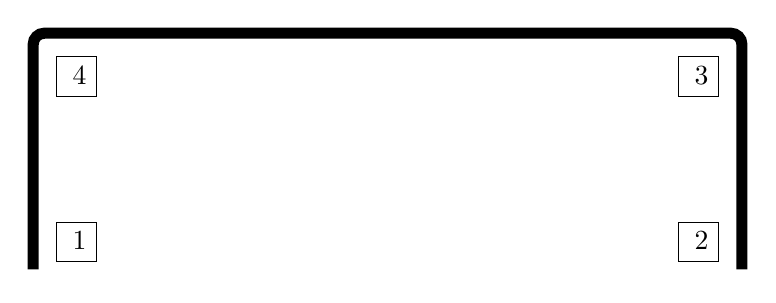
\begin{tikzpicture}[>=stealth]
			\draw[line width =4pt, rounded corners] (0,0)--(0,3)--(9,3)--(9,0);
			\draw (0.3,0.1) rectangle (0.8,0.6) node[below left]{$1$};
			\draw (0.3,2.2) rectangle (0.8,2.7) node[below left]{$4$};
			\draw (8.2,0.1) rectangle (8.7,0.6) node[below left]{$2$};
			\draw (8.2,2.2) rectangle (8.7,2.7) node[below left]{$3$};
			
		\end{tikzpicture}
		\hspace*{-5.5cm}
\begin{tikzpicture}[y=0.80pt, x=0.80pt, yscale=-1, xscale=1, inner sep=0pt, outer sep=0pt,scale=0.9]
			\begin{scope}[shift={(0,99.0)},xscale=0.100,yscale=-0.100,fill=black]
				\path[fill] (480,862) .. controls (441,823) and
				(441,787) .. (479,749) .. controls (507,722) and
				(507,720) .. (485,726) .. controls (471,729) and
				(446,723) .. (420,710) .. controls (364,681) and
				(307,661) .. (245,646) .. controls (202,636) and
				(195,631) .. (195,610) .. controls (195,587) and
				(198,585) .. (235,589) .. controls (257,591) and
				(304,603) .. (340,617) .. controls (376,630) and
				(413,644) .. (423,647) .. controls (438,652) and
				(440,643) .. (440,554) -- (440,456) --
				(402,411) .. controls (348,347) and (344,336) ..
				(336,241) .. controls (329,150) and (336,130) ..
				(375,130) .. controls (408,130) and (417,147) ..
				(424,231) .. controls (431,301) and (435,310) ..
				(476,363) .. controls (501,394) and (527,420) ..
				(533,420) .. controls (540,420) and (566,394) ..
				(591,362) .. controls (635,308) and (637,301) ..
				(644,226) .. controls (650,144) and (658,130) ..
				(697,130) .. controls (732,130) and (739,156) ..
				(729,253) .. controls (721,337) and (718,344) ..
				(675,399) -- (630,456) -- (630,554) .. controls
				(630,662) and (629,661) .. (702,624) .. controls
				(740,605) and (849,580) .. (866,587) .. controls
				(874,590) and (880,602) .. (878,613) .. controls
				(876,629) and (862,636) .. (817,647) .. controls
				(785,654) and (725,675) .. (683,695) .. controls
				(641,714) and (600,730) .. (592,730) .. controls
				(579,730) and (579,732) .. (592,748) .. controls
				(618,776) and (622,807) .. (606,839) .. controls
				(588,874) and (585,875) .. (543,885) .. controls
				(515,891) and (506,887) .. (480,862) -- cycle;
			\end{scope}
			
		\end{tikzpicture}
	\end{center}
	\loigiai{
		Gọi $A_i$ là biến cố cầu thủ sút vào vị trí $i$, $B_i$là biến cố thủ môn bay người đến vị trí $i$ ($i=1,2,3,4$). Dễ thấy $\mathrm{P}(A_i)=\mathrm{P}(B_i)=\dfrac{1}{4}$. Gọi $C$ là biến cố cú sút không vào lưới. Ta có
		\begin{align*}
			\mathrm{P}(C)=\mathrm{P}(A_1)\mathrm{P}(B_1)+ \mathrm{P}(A_2)\mathrm{P}(B_2) + \dfrac{1}{2}\mathrm{P}(A_3)\mathrm{P}(B_3)+ \dfrac{1}{2}\mathrm{P}(A_4)\mathrm{P}(B_4)=\dfrac{3}{16}=0{,}1875.
		\end{align*}
	}
\end{bt}

\begin{bt}%[1D9H2-4]
% nguon: Archive/2024/Update-SP-BG10-11-3/SP-3/BG11-3/data_1C5/Bai-2-Dang-3-Tinhxacsuatbangdinhnghia-Quan-On.tex #1588
[Mức 2]%[BG Toán 11 CT2025, Quan Ón]
	Đề cương ôn tập học kỳ I môn Lịch sử lớp $ 11 $ có $ 20 $ câu hỏi. Đề thi học kỳ I gồm $ 3 $ câu hỏi trong $ 20 $ câu hỏi đó. Một học sinh chỉ ôn $ 10 $ câu trong đề cương. Giả sử các câu hỏi trong đề cương đều có khả năng được chọn làm câu hỏi thi như nhau. Hãy tính xác suất để có ít nhất $ 2 $ câu hỏi của đề thi học kỳ I nằm trong số $ 10 $ câu hỏi mà học sinh nói trên đã ôn.	
	\loigiai{
		Không gian mẫu $ \Omega $ là tập hợp các cách chọn 	$ 3 $ câu trong đề cương làm đề thi.\\
		Ta có $n(\Omega) = \mathrm{C}^3_{20} = 1140$.\\
		Gọi $ A $ là biến cố \lq\lq Có ít nhất $2$ câu hỏi của đề thi học kỳ I nằm trong số $ 10 $ câu hỏi mà học sinh nói trên đã ôn\rq\rq.\\
		Ta có $ n(A) = \mathrm{C}^2_{10} \cdot \mathrm{C}^1_{10} + \mathrm{C}^3_{10} = 570 $.\\
		Vậy xác suất cần tìm là $ \mathrm{P}(A) = \dfrac{n(A)}{n(\Omega)} = \dfrac{570}{1140} = \dfrac{1}{2} $.
	}		
\end{bt}

\begin{bt}%[1D9H2-4]
% nguon: Archive/2024/Update-SP-BG10-11-3/SP-3/BG11-3/data_1C5/Bai-2-Dang-3-Tinhxacsuatbangdinhnghia-Quan-On.tex #1591
[Mức 2]
	Gieo một con xúc xắc cân đối đồng chất $ 2 $ lần. Tính xác suất biến cố A: \lq\lq Hai lần xuất hiện mặt có số chấm chấm giống nhau\rq\rq.
	\loigiai{
		Gọi $ \Omega $ là không gian mẫu, suy ra số phần tử không gian mẫu là $ n(\Omega) = 36$.\\
		Ta có $ n(A) = 6 $.\\
		Suy ra xác suất $ \mathrm{P}(A) = \dfrac{n(A)}{n(\Omega)} = \dfrac{1}{6}$.
	}
\end{bt}

\begin{bt}%[1D9H2-4]
% nguon: Archive/2024/Update-SP-BG10-11-3/SP-3/BG11-3/data_1C5/Bai-2-Dang-3-Tinhxacsuatbangdinhnghia-Quan-On.tex #1592
[Mức 2]
	Để kiểm tra chất lượng từ một công ty sữa, người ta gửi đến bộ phận kiểm nghiệm $5$ hộp sữa cam, $4$ hộp sữa dâu và $3$ hộp sữa nho. Bộ phận kiểm nghiệm chọn ngẫu nhiên $3$ hộp sữa để phân tích mẫu. Tính xác suất để ba hộp sữa được chọn có cả ba loại.
	\loigiai{
		Chọn ngẫu nhiên 3 hộp sữa trong 12 hộp sữa để phân tích mẫu nên $n(\Omega) = \mathrm{C}_{12}^3 = 220$.\\
		Gọi $A$ là biến cố: \lq\lq Cả ba hộp sữa được chọn có cả ba loại\rq\rq, ta có $n(A) = \mathrm{C}_5^1 \cdot \mathrm{C}_4^1 \cdot \mathrm{C}_3^1 = 60$.\\
		Xác suất để ba hộp sữa được chọn có cả ba loại là $\mathrm{P}(A) = \dfrac{n(A)}{n(\Omega)} = \dfrac{60}{220} = \dfrac{3}{11}$.
	}
\end{bt}

\begin{bt}%[1D9H2-4]
% nguon: Archive/2024/Update-SP-BG10-11-3/SP-3/BG11-3/data_1C5/Bai-2-Dang-3-Tinhxacsuatbangdinhnghia-Quan-On.tex #1593
[Mức 2]
	Một tổ có $10$ học sinh trong đó có $4$ học sinh nữ và $6$ học sinh nam. Cần chọn 4 học sinh, tính xác suất sao cho chọn được $4$ học sinh có cả nam và nữ.
	\loigiai{	
		Số cách chọn $4$ học sinh bất kỳ là $\mathrm{C}_{10}^4 = 210$ cách.\\
		Số cách chọn được $4$ học sinh toàn là nam hoặc toàn là nữ là $\mathrm{C}_{4}^4 + \mathrm{C}_{6}^4 = 16$ cách.\\
		Vậy số cách chọn được $4$ học sinh trong đó cả nam và nữ là $210 - 16 = 194$.\\
		Xác suất cần tìm là $\dfrac{194}{210} = \dfrac{97}{105}$.	
	}
\end{bt}

\begin{bt}%[1D9H2-4]
% nguon: Archive/2024/Update-SP-BG10-11-3/SP-3/BG11-3/data_1C5/Bai-2-Dang-3-Tinhxacsuatbangdinhnghia-Quan-On.tex #1594
[Mức 2]
	Có $40$ tấm thẻ đánh số thứ tự từ $1$ đến $40$. Chọn ngẫu nhiên ra $10$ tấm thẻ. Tính xác suất để lấy được $5$ tấm thẻ mang số lẻ, $5$ tấm thẻ mang số chẵn trong đó có đúng một thẻ mang số chia hết cho $6$.
	\loigiai{
		Rút ngẫu nhiên $10$ tấm thẻ từ $40$ tấm thẻ có $\mathrm{C}_{40}^{10}$ cách.\\
		Từ số $1$ đến số $40$ có $6$ số chia hết cho $6$ là $6$, $12$, $18$, $24$, $30$, $36$.\\
		Chọn $1$ số chia hết cho $6$ có $6$ cách.\\
		Rút $4$ số chẵn có $\mathrm{C}_{14}^4$ cách.\\
		Rút $5$ số lẻ có $\mathrm{C}_{20}^5$ cách.\\
		Vậy xác suất cần tìm là 
		$ \mathrm{P} = \dfrac{6\cdot\mathrm{C}_{14}^4\cdot\mathrm{C}_{20}^5 }{\mathrm{C}_{40}^{10}} = \dfrac{126}{1147}$.
	}
\end{bt}

\begin{bt}%[1D9V2-4]
% nguon: Archive/2024/Update-SP-BG10-11-3/SP-3/BG11-3/data_1C5/Bai-2-Dang-3-Tinhxacsuatbangdinhnghia-Quan-On.tex #1595
[Mức 3]
	Một đoàn tàu có $6$ toa ở sân ga. Có $6$ hành khách từ sân ga lên tàu, mỗi người độc lập với nhau và chọn một toa một cách ngẫu nhiên. Tính xác suất để một toa có $1$ người lên, một toa có $2$ người lên, một toa có $3$ người lên và ba toa không có người nào lên.
	\loigiai{
		Do mỗi người độc lập và có $6$ cách chọn toa tàu để lên nên kích thước của không gian mẫu là $	|\Omega| = 6^6$.\\
		Ta chia ra ba bước để xếp $6$ người vào $6$ toa thoả mãn yêu cầu bài toán như sau
		\begin{itemize}
			\item Chọn $1$ toa làm toa $1$ người và chọn người để ngồi toa đó có $6\cdot 6 = 36$ cách;
			\item Chọn $1$ toa làm toa $2$ người trong $5$ toa còn lại và chọn $2$ người trong $5$ người còn lại có $5\cdot \mathrm{C}^2_5 = 50$ cách;
			\item Chọn $1$ toa cho $3$ người còn lại trong $4$ toa còn lại có $4$ cách.
		\end{itemize}
		Do đó số cách xếp $6$ người vào $6$ toa thoả mãn bài ra là $36\cdot 50 \cdot 4 = 7200$ cách.\\
		Vậy xác suất cần tìm là $\dfrac{7200}{6^6} = \dfrac{25}{162}$.
	}
\end{bt}

\begin{ex}%[1D9V2-3]
% nguon: Archive/2024/Update-SP-BG10-11-3/SP-3/BG11-3/data_1C5/Bai-2-Dang-3-Tinhxacsuatbangdinhnghia-Quan-On.tex #1600
[Mức 3]%[BG Toán 11 CT2025, Quan Ón]
	Lớp 10A1 có $35$ học sinh gồm $20$ học sinh nữ và $15$ học sinh nam. Nhà trường cần chọn $3$ học sinh của lớp đó tham gia trồng cây. Các khẳng định sau đây, khẳng định nào là đúng, khẳng định nào là sai?
	\choiceTF[t]
	{\True Xác suất để $3$ học sinh được chọn có đúng một học sinh nữ bằng $\dfrac{60}{187}$}
	{\True Xác suất để $3$ học sinh được chọn có đúng hai học sinh nữ bằng $\dfrac{570}{1309}$}
	{Xác suất để $3$ học sinh được chọn có ít nhất một học sinh nữ bằng $\dfrac{90}{119}$}
	{Xác suất để $3$ học sinh được chọn có nhiều nhất hai học sinh nữ bằng $\dfrac{114}{187}$}
	\loigiai{
		Ta có số phần tử không gian mẫu $n(\Omega) = \mathrm{C}_{35}^3$.
		\begin{itemchoice}
			\itemch  Gọi $A$: \lq \lq $3$ học sinh được chọn đúng một học sinh nữ\rq \rq.\\
			Ta có $n(A) = 20 \cdot \mathrm{C}_{15}^2$.\\
			Xác suất của biến cố $A$ là $\mathrm{P}(A)=\dfrac{n(A)}{n(\Omega)}=\dfrac{20 \cdot \mathrm{C}_{15}^2}{\mathrm{C}_{35}^3}=\dfrac{60}{187}$.
			\itemch  Gọi $B$: \lq \lq $3$ học sinh được chọn đúng hai học sinh nữ\rq \rq. \\
			Ta có $n(B)=\mathrm{C}_{20}^2 \cdot 15$.\\
			Xác suất của biến cố $B$ là $\mathrm{P}(B)=\dfrac{n(A)}{n(\Omega)}=\dfrac{\mathrm{C}_{20}^2 \cdot 15}{\mathrm{C}_{35}^3}=\dfrac{570}{1309}$.
			\itemch  Gọi $C$: \lq \lq $3$ học sinh được chọn có ít nhất một học sinh nữ\rq \rq.\\
			Ta có  $n(C)=20\cdot \mathrm{C}_{15}^2+\mathrm{C}_{20}^2 \cdot 15 +\mathrm{C}_{20}^3$.\\
			Xác suất của biến cố $C$ là $\mathrm{P}(C)=\dfrac{n(C)}{n(\Omega)}=\dfrac{20\cdot \mathrm{C}_{15}^2+\mathrm{C}_{20}^2 \cdot 15 +\mathrm{C}_{20}^3}{\mathrm{C}_{35}^3}=\dfrac{174}{187}$.
			\itemch  Gọi $D$: \lq \lq $3$ học sinh được chọn có nhiều nhất hai học sinh nữ\rq \rq.\\
			Ta có $n(D)=\mathrm{C}_{15}^3+20\cdot \mathrm{C}_{15}^2+\mathrm{C}_{20}^2 \cdot 15$.\\
			Xác suất của biến cố $D$ là $\mathrm{P}(D)=\dfrac{n(D)}{n(\Omega)}=\dfrac{\mathrm{C}_{15}^3+20\cdot \mathrm{C}_{15}^2+\mathrm{C}_{20}^2 \cdot 15}{\mathrm{C}_{35}^3}=\dfrac{1081}{1309}$.
		\end{itemchoice}
	}
\end{ex}

\begin{ex}%[1D9V2-3]
% nguon: Archive/2024/Update-SP-BG10-11-3/SP-3/BG11-3/data_1C5/Bai-2-Dang-3-Tinhxacsuatbangdinhnghia-Quan-On.tex #1601
[Mức 3]%[BG Toán 11 CT2025, Quan Ón]
	Một đội tình nguyện gồm $6$ học sinh khối $10$, $5$ học sinh khối $11$ và $4$ học sinh khối $12$. Chọn ngẫu nhiên $5$ học sinh trong đội. Các khẳng định sau đây, khẳng định nào đúng, khẳng định nào sai?
	\choiceTF[t]
	{Số phần tử không gian mẫu là $15$ phần tử}
	{\True Số phần tử của biến cố \lq\lq Cả $5$ học sinh được chọn học cùng một khối\rq \rq \, là $\mathrm{C}_ 6^5+\mathrm{C}_ 5^5$ phần tử}
	{Xác suất của biến cố \lq\lq Cả $5$ học sinh được chọn học cùng một khối\rq \rq \, là $\dfrac{5}{3003}$}
	{\True Xác suất của biến cố \lq\lq Chọn được $5$ học sinh đủ ba khối\rq \rq \, là $\dfrac{310}{429}$}
	\loigiai{
		Số cách chọn $5$ học sinh trong $15$ học sinh là $\mathrm{C}_{15}^5=3003$ cách.
		\begin{itemchoice}
			\itemch  Số phần tử không gian mẫu là $n(\Omega)=\mathrm{C}_{15}^5=3003$.
			\itemch  Gọi $A$ là biến cố \lq\lq Cả $5$ học sinh được chọn học cùng một khối\rq \rq.\\
			Vì cả $5$ học sinh được chọn học cùng một khối nên chỉ có thể chọn $5$ học sinh khối $10$ hoặc $5$ học sinh khối $11$. Suy ra $n(A)=\mathrm{C}_6^5+\mathrm{C}_5^5$.
			\itemch  Xác suất của biến cố \lq\lq Cả $5$ học sinh được chọn học cùng một khối\rq \rq \ là
			$$\mathrm{P}(A)=\dfrac{n(A)}{n(\Omega)}=\dfrac{\mathrm{C}_6^5+\mathrm{C}_5^5}{\mathrm{C}_{15}^5}=\dfrac{1}{429}.$$
			\itemch  Gọi $B$ là biến cố \lq\lq Chọn được $5$ học sinh đủ ba khối\rq \rq. Khi đó\\
			$n(B)=\mathrm{C}_6^1\cdot \mathrm{C}_5^1\cdot \mathrm{C}_4^3 + \mathrm{C}_6^1\cdot \mathrm{C}_5^3\cdot \mathrm{C}_4^1 + \mathrm{C}_6^1\cdot \mathrm{C}_5^2\cdot \mathrm{C}_4^2 + \mathrm{C}_6^2\cdot \mathrm{C}_5^1\cdot \mathrm{C}_4^2 + \mathrm{C}_6^2\cdot \mathrm{C}_5^2\cdot \mathrm{C}_4^1 + \mathrm{C}_6^3\cdot \mathrm{C}_5^1\cdot \mathrm{C}_4^1 = 2170$.\\
			Vậy $\mathrm{P}(B) = \dfrac{n(B)}{n(\Omega)} = \dfrac{2170}{3003} = \dfrac{310}{429}$.
		\end{itemchoice}
	}
\end{ex}

\begin{bt}%[1D9V2-4]
% nguon: Archive/2024/Update-SP-BG10-11-3/SP-3/BG11-3/data_1C5/Bai-2-Dang-3-Tinhxacsuatbangdinhnghia-Quan-On.tex #1604
[Mức 3]
	Xếp $6$ học sinh nam và $4$ học sinh nữ vào một bàn tròn có $10$ ghế. Tính xác suất để không có hai học sinh nữ ngồi cạnh nhau (kết quả làm tròn đến hàng phần trăm).
	\shortans{$0{,}12$}
	\loigiai{
		Cố định $1$ vị trí cho một học sinh nam (hoặc nữ), đánh dấu các ghế còn lại từ $1$ đến $9$.\\
		Không gian mẫu là hoán vị của $9$ học sinh (còn lại, không cố định) trên $9$ ghế đánh dấu.\\
		Suy ra số phần tử không gian mẫu là $n(\Omega)=9!$.\\
		Gọi $A$ là biến cố \lq\lq Không có hai học sinh nữ ngồi cạnh nhau\rq\rq.\\
		Ta mô tả khả năng thuận lợi của biến cố $A$ như sau
		\begin{itemize}
			\item Đầu tiên, ta cố định một học sinh nam, $5$ học sinh còn lại có $5!$ cách sắp xếp.
			\item Sau đó, sắp $4$ bạn nữ vào $4$ trong $6$ khoảng trống giữa hai bạn nam có $\mathrm{A}_6^4$ cách.
		\end{itemize}
		Suy ra số phần tử của biến cố $A$ là $n(A) = 5!\cdot \mathrm{A}_6^4$.\\
		Vậy $P(A) = \dfrac{n(A)}{n(\Omega)} = \dfrac{5!\cdot \mathrm{A}_6^4}{9!} = \dfrac{5}{42} \approx 0{,}12$.
	}
\end{bt}

\begin{bt}%[1D9H1-3]
% nguon: Archive/2024/Update-SP-BG10-11-3/SP-3/BG11-3/data_1C5/DS11-C5-B2-Dang5-TinhXacSuatBangQuyTacNhan-TranTony.tex #1607
%[Bài giảng 11, Trần Tony]
	Gieo đồng thời một đồng xu và một con súc sắc. Xác suất để đồng xu xuất hiện mặt sấp là $0{,}5$ và xác suất để con súc sắc xuất hiện mặt chẵn chấm là $0{,}5$. Tính xác suất để đồng xu xuất hiện mặt ngửa và con súc sắc xuất hiện mặt chẵn chấm.
	\loigiai{
		Vì xác suất đồng xu xuất hiện mặt sấp là $0{,}5$ nên xác suất để đồng xu xuất hiện mặt ngửa là $\mathrm{P}(A)=0{,}5$.\\
		Gọi $\mathrm{P}(B)=0{,}5$ là xác suất để con súc sắc xuất hiện mặt chẵn chấm.\\
		Do xác suất xuất hiện mặt chẵn hoặc lẻ của đồng xu độc lập với sự xuất hiện các mặt của con súc sắc nên ta có $$\mathrm{P}\left(A\cap B\right)=\mathrm{P}(A)\cdot\mathrm{P}(B)=0{,}5\cdot0{,}5=0{,}25.$$
	}
\end{bt}

\begin{ex}%[1D9V1-3]
% nguon: Archive/2024/Update-SP-BG10-11-3/SP-3/BG11-3/data_1C5/DS11-C5-B2-Dang5-TinhXacSuatBangQuyTacNhan-TranTony.tex #1610
%[Bài giảng 11, Trần Tony]
	Cho ba hộp giống nhau, mỗi hộp $7$ bút chỉ khác nhau về màu sắc.\\
	Hộp thứ nhất: Có $3$ bút màu đỏ, $2$ bút màu xanh, $2$ bút màu đen;\\
	Hộp thứ hai: Có $2$ bút màu đỏ, $2$ màu xanh, $3$ màu đen;\\
	Hộp thứ ba: Có $5$ bút màu đỏ, $1$ bút màu xanh, $1$ bút màu đen.
	\choiceTF[t]
	{\True Lấy ngẫu nhiên một hộp, xác suất lấy được hộp thứ nhất là $\dfrac{1}{3}$}
	{Số cách lấy $2$ bút từ $7$ bút là $\mathrm{A}_7^2$}
	{Rút từ hộp thứ nhất ra $2$ bút, xác suất của biến cố "rút được hai bút ở hộp thứ nhất không có màu đen" là $\dfrac{10}{63}$}
	{\True Lấy ngẫu nhiên một hộp, rút từ hộp đó ra $2$ bút. Xác suất của biến cố “Lấy được hai bút không có màu đen” là $\dfrac{31}{63}$}
	\loigiai{		
		\begin{itemchoice}
			\itemch  Xác suất lấy được hộp thứ nhất là $\dfrac{1}{3}$.
			\itemch  Số cách lấy $2$ bút từ $7$ bút là $\mathrm{C}_7^2$.
			\itemch  Xác suất của biến cố "rút được hai bút ở hộp thứ nhất không có màu đen" là $\dfrac{\mathrm{C}_5^2}{\mathrm{C}_7^2}=\dfrac{10}{21}$
			\itemch 
			Gọi $A_i$ là biến cố rút hai bút ở hộp thứ $i$ không có màu đen.\\
			Ta thấy các biến cố $A_1$; $A_2$; $A_3$ đôi một xung khắc với nhau.\\
			Xác suất lấy được hộp thứ $1$ là $\dfrac{1}{3}$.\\
			Tương tự; xác suất để lấy được hộp thứ $2$; thứ $3$ cũng là $\dfrac{1}{3}$.\\
			Ta có $P(A_1)=\dfrac{\mathrm{C}_5^2}{\mathrm{C}_7^2}$, $P(A_2)=\dfrac{\mathrm{C}_4^2}{\mathrm{C}_7^2}$, $P(A_3)=\dfrac{\mathrm{C}_6^2}{\mathrm{C}_7^2}$.\\
			Xác suất cần tính $P=\dfrac{1}{3}P(A_1)+\dfrac{1}{3}P(A_2)+\dfrac{1}{3}P(A_3)=\dfrac{31}{63}$.
		\end{itemchoice}
	}
\end{ex}

\begin{bt}%[1D9H1-3]
% nguon: Archive/2024/Update-SP-BG10-11-3/SP-3/BG11-3/data_1C5/DS11-C5-B2-Dang5-TinhXacSuatBangQuyTacNhan-TranTony.tex #1612
%[Bài giảng 11, Trần Tony]
	Hai đội bóng $A$ và $B$ nằm ở hai bảng đấu khác nhau của một giải đấu bóng đá. Biết rằng xác suất để hai đội vào vòng chung kết lần lượt là $0{,}26$ và $0{,}34$. Biết rằng mỗi bảng đấu chỉ có một đội lọt vào vòng chung kết. Tính xác suất để hai đội $A$ và $B$ đều lọt vào vòng chung kết.
	\loigiai{
		Gọi xác suất của đội $A$ và $B$ vào chung kết lần lượt là $\mathrm{P}(A)=0{,}26$, $\mathrm{P}(B)=0{,}34$.\\
		Xác suất để cả hai đội đều lọt vào chung kết là $\mathrm{P}(A\cap B)=0{,}26\cdot 0{,}34=0{,}0884=8{,}84\%$.
	}
\end{bt}

\begin{bt}%[1D9H1-3]
% nguon: Archive/2024/Update-SP-BG10-11-3/SP-3/BG11-3/data_1C5/DS11-C5-B2-Dang5-TinhXacSuatBangQuyTacNhan-TranTony.tex #1613
%[Bài giảng 11, Trần Tony]
	Một đề kiểm tra $5$ phút có hai câu trắc nghiệm. Biết xác suất đúng mỗi câu là $0{,}25$. Tính xác suất để một học sinh không học bài có thể khoang đúng được cả hai câu.
	\loigiai{
		Gọi xác suất để học sinh khoanh đúng hai câu hỏi lần lượt là $\mathrm{P}(A)=\mathrm{P}(B)=0{,}25$.\\
		Vì mỗi biến cố là độc lập với nhau nên ta có xác suất cần tìm là $\mathrm{P}(A\cap B)=0{,}25\cdot 0{,}25=0{,}0625$.
	}
\end{bt}

\begin{bt}%[1D9H1-3]
% nguon: Archive/2024/Update-SP-BG10-11-3/SP-3/BG11-3/data_1C5/DS11-C5-B2-Dang5-TinhXacSuatBangQuyTacNhan-TranTony.tex #1614
%[Bài giảng 11, Trần Tony]
	Hai đội công nhân trong một nhà máy sản xuất có xác suất tạo ra sản phẩm tốt lần lượt là $0{,}75$ và $0{,}85$. Tính xác suất phế phẩm mà nhà máy đó tạo ra bởi cả hai đội.
	\loigiai{
		Gọi xác suất tạo ra sản phẩm tốt của hai đội công nhân lần lượt là $\mathrm{P}(A)=0{,}75$ và $\mathrm{P}(B)=0{,}85$.\\
		Gọi xác suất tạo ra phế phẩm của hai đội công nhân lần lượt là $\mathrm{P}(\overline{A})=0{,}25$ và $\mathrm{P}(\overline{B})=0{,}15$.\\
		Vậy xác suất phế phẩm mà nhà máy đó tạo ra bỏi cả hai đội là
		$$\mathrm{P}\left(\overline{A}\cap \overline{B}\right)=0{,}25\cdot 0{,}15=0{,}0375.$$
	}
\end{bt}

\begin{bt}%[1D9H1-3]
% nguon: Archive/2024/Update-SP-BG10-11-3/SP-3/BG11-3/data_1C5/DS11-C5-B2-Dang5-TinhXacSuatBangQuyTacNhan-TranTony.tex #1615
%[Bài giảng 11, Trần Tony]
	Hai bạn An và Minh cùng tham gia giải cờ vua cấp tỉnh. Biết rằng hai bạn không ở chung $1$ bảng và mỗi bảng chỉ có một người vô vòng chung kết. Biết xác suất vô vòng chung kết của An và Minh lần lượt là $0{,}35$ và $0{,}45$. Tính xác suất để An và Minh cùng vô vòng chung kết.
	\loigiai{
		Gọi xác suất để An và Minh vô vòng chung kết lần lượt là $\mathrm{P}(A)=0{,}35$ và $\mathrm{P}(B)=0{,}45$.\\
		Vậy xác suất để cả hai bạn cùng vô vòng chung kết là $\mathrm{P}(A\cap B)=0{,}35\cdot 0{,}45=0{,}1575$.
	}
\end{bt}

\begin{bt}%[1D9H1-3]
% nguon: Archive/2024/Update-SP-BG10-11-3/SP-3/BG11-3/data_1C5/DS11-C5-B2-Dang5-TinhXacSuatBangQuyTacNhan-TranTony.tex #1616
%[Bài giảng 11, Trần Tony]
	Một nhà máy có hai tổ máy sản xuất một mặt hàng, biết rằng xác suất để hai tổ máy phải nghỉ để bảo dưỡng lần lượt là $0{,}2$ và $0{,}32$. Tính xác suất để cả hai tổ máy đều hoạt động.
	\loigiai{
		Gọi xác suất để hai tổ máy phải nghỉ để bảo dưỡng lần lượt là $\mathrm{P}(A)=0{,}2$ và $\mathrm{P}(B)=0{,}32$.\\
		Nên xác suất để hai tổ máy đều hoạt động là $\mathrm{\overline{A}}=0{,}8$ và $\mathrm{\overline{B}}=0{,}68$.\\
		Vậy xác suất để cả hai tổ máy đều hoạt động là $\mathrm{P}\left(\overline{A}\cap \overline{B}\right)=0{,}8\cdot 0{,}68=0{,}544$.
	}
\end{bt}

\begin{ex}%[1D9V1-3]
% nguon: Archive/2024/Update-SP-BG10-11-3/SP-3/BG11-3/data_1C5/DS11-C5-B2-Dang5-TinhXacSuatBangQuyTacNhan-TranTony.tex #1618
%[Bài giảng 11, Trần Tony]
	Hai bạn An và Hà của lớp 11A tham gia giải bóng bàn đơn nữ do nhà trường tổ chức. Hai bạn đó nằm ở hai bảng đấu loại khác nhau, mỗi bảng đấu loại chỉ chọn một người vào vòng chung kết. Xác suất lọt qua vòng loại để vào vòng chung kết của An và Hà lần lượt là $0{,}6$ và $0{,}7$.
	\choiceTF[t]
	{\True Biến cố "Bạn An lọt vào vòng chung kết" và biến cố "Bạn Hà lọt vào vòng chung kết" là hai biến cố độc lập}
	{\True Xác suất cả hai bạn lọt vào vòng chung kết là $0{,}42$}
	{Xác suất có ít nhất một bạn lọt vào vòng chung kết là $0{,}8$}
	{Xác suất chỉ có bạn Hà lọt vào vòng chung kết là $0{,}7$}
	\loigiai{
		\begin{itemchoice}
			\itemch  Biến cố "Bạn An lọt vào vòng chung kết" và biến cố "Bạn Hà lọt vào vòng chung kết" là hai biến cố độc lập.
			\itemch  Xác suất cả hai bạn lọt vào vòng chung kết là $0{,}6\cdot 0{,}7=0{,}42$.
			\itemch  
			Xác suất không lọt vào vòng chung kết của An là $0{,}4$.\\
			Xác suất không lọt vào vòng chung kết của Hà là $0{,}3$.\\			
			Xác suất không có bạn nào lọt vào vòng chung kết là $0{,}4\cdot 0{,}3=0{,}12$.\\
			Xác suất có ít nhất một bạn nào lọt vào vòng chung kết là $1-0{,}12=0{,}88$.
			\itemch  Xác suất chỉ có bạn Hà lọt vào vòng chung kết là $0{,}7\cdot 0{,}4=0{,}28$.
		\end{itemchoice}
	}
\end{ex}

\begin{ex}%[1D9V1-3]
% nguon: Archive/2024/Update-SP-BG10-11-3/SP-3/BG11-3/data_1C5/DS11-C5-B2-Dang5-TinhXacSuatBangQuyTacNhan-TranTony.tex #1620
%[Bài giảng 11, Trần Tony]
	Có $6$ bạn nam trong đó có Hoàng và $3$ bạn nữ xếp ngẫu nhiên thành một hàng ngang.
	\choiceTF[t]
	{Số cách xếp $9$ bạn thành hàng ngang là $4320$}
	{\True Số cách xếp $9$ bạn thành hàng ngang mà bạn Hoàng đứng ngoài cùng là $80640$}
	{Số cách xếp $9$ bạn thành hàng ngang mà $6$ bạn nam luôn đứng cạnh nhau là $4320$}
	{\True Xác suất để không có hai bạn nữ nào đứng cạnh nhau và Hoàng đứng ở ngoài cùng bằng $\dfrac{5}{63}$}
	\loigiai{
	\begin{itemchoice}
		\itemch  Số cách xếp $9$ bạn thành hàng ngang là $9!=362880$.
		\itemch  Số cách xếp $9$ bạn thành hàng ngang mà bạn Hoàng đứng ngoài cùng là $2\cdot 8!=80640$.
		\itemch  Số cách xếp $9$ bạn thành hàng ngang mà $6$ bạn nam luôn đứng cạnh nhau là $6!\cdot 4!=17280$.
		\itemch 
			\begin{itemize}
				\item Số cách xếp tùy ý $9$ bạn thành hàng ngang là $9!$ $\Rightarrow n(\Omega)=9!$.
				\item Số cách xếp sao cho không có hai bạn nữ nào đứng cạnh nhau và Hoàng đứng ở ngoài cùng
				\begin{itemize}
					\item Xếp $6$ bạn nam thành một hàng ngang sao cho Hoàng đứng ở ngoài cùng, có $2\cdot 5!$ cách.
					\item Xếp 3 bạn nữ vào 6 khoảng trống tạo bởi 6 bạn nam đã được xếp, trừ khoảng trống ngoài cùng bên cạnh Hoàng, có $\mathrm{A}_6^3$ cách.
				\end{itemize}
			\end{itemize}
			Vậy số cách xếp để không có hai bạn nữ nào đứng cạnh nhau và Hoàng đứng ở ngoài cùng bằng: $2\cdot 5 ! \cdot \mathrm{A}_6^3$. Suy ra, xác suất để không có hai bạn nữ nào đứng cạnh nhau và Hoàng đứng ở ngoài cùng bằng $\dfrac{2\cdot 5! \cdot \mathrm{A}_6^3}{n(\Omega)}=\dfrac{2\cdot 5! \cdot  \mathrm{A}_6^3}{9!}=\dfrac{5}{63}$.
	\end{itemchoice}
	}
\end{ex}

\begin{bt}%[1D9V1-3]
% nguon: Archive/2024/Update-SP-BG10-11-3/SP-3/BG11-3/data_1C5/DS11-C5-B2-Dang5-TinhXacSuatBangQuyTacNhan-TranTony.tex #1622
%[Bài giảng 11, Trần Tony]
	Trong một trò chơi trên truyền hình có một bộ câu hỏi gồm $6$ câu hỏi trắc nghiệm khách quan. Mỗi câu có $4$ phương án trả lời, trong đó chỉ có một phương án đúng. Một người chơi trả lời bộ câu hỏi bằng cách chọn ngẫu nhiên một phương án trả lời ở mỗi câu hỏi. Tính xác suất để người đó trả lời đúng $3$ câu. 
	\shortans{$0{,}13$}
	\loigiai{
		Gọi $A_i$ là biến cố trả lời đúng câu thứ $i$ với $i=1,2,\ldots,6$. Suy ra $\mathrm{P}(A_i)=\dfrac{1}{4}$, $\mathrm{P}(\overline{A_i})=\dfrac{3}{4}$.\\
		 xác suất để người đó trả lời đúng $3$ câu là $P=\mathrm{C}_6^3\left(\dfrac{1}{4}\right)^3\left(\dfrac{3}{4}\right)^3\approx 0{,}13$.
	}
\end{bt}

\begin{bt}%[1D9C1-3]
% nguon: Archive/2024/Update-SP-BG10-11-3/SP-3/BG11-3/data_1C5/DS11-C5-B2-Dang5-TinhXacSuatBangQuyTacNhan-TranTony.tex #1623
%[Bài giảng 11, Trần Tony]
	Có $3$ xạ thủ cùng bắn vào bia với xác suất bắn trúng bia của mỗi xạ thủ lần lượt là $0{,}7$; $0{,}6$ và $0{,}5$. Tính xác suất để có ít nhất $1$ người bắn trúng bia (kết quả làm tròn đến hàng phần trăm).
	\shortans{$0{,}94$}
	\loigiai{
		Gọi $A_1$ là biến cố: ``xạ thủ thứ $1$ bắn trúng'' $\Rightarrow\mathrm{P}(A_1)=0,7$.\\
		Khi đó $\overline{A_1}$ là biến cố: ``xạ thủ thứ nhất bắn không trúng'' $\Rightarrow\mathrm{P}(\overline{A_1})=0{,}3$.\\
		Tương tự: $\mathrm{P}(A_2)=0{,}6$, $\mathrm{P}(\overline{A_2})=0{,}4$, $\mathrm{P}(A_3)=\mathrm{P}(\overline{A_3})=0{,}5$.\\
		Gọi $B$ là biến cố: ``cả $3$ người không bắn trúng bia''.\\
		Khi đó $\overline{B}$ là biến cố: ``có ít nhất $1$ người bắn trúng bia''.\\
		$\mathrm{P}(B)=\mathrm{P}\left(\overline{A_1}\overline{A_2}\overline{A_3}\right)=\mathrm{P}\left(\overline{A_1}\right)\times\mathrm{P}\left(\overline{A_2}\right)\times\mathrm{P}\left(\overline{A_3}\right)=0{,}3\times0{,}4\times0{,}5=0{,}06\\
		\Rightarrow\mathrm{P}\left(\overline{B}\right)=1-0{,}06=0{,}94$.
		}
\end{bt}

\begin{bt}%[1D9C1-3]
% nguon: Archive/2024/Update-SP-BG10-11-3/SP-3/BG11-3/data_1C5/DS11-C5-B2-Dang5-TinhXacSuatBangQuyTacNhan-TranTony.tex #1624
%[Bài giảng 11, Trần Tony]
	Một công nhân phải theo dõi và can thiệp hoạt động của hai máy dệt A và B. Trong một giờ, xác suất để máy dệt A hỏng là $\dfrac{1}{7}$; xác suất máy dệt B hỏng là $\dfrac{1}{5}$. Tính xác suất để người công nhân không phải can thiệp máy nào trong một giờ (kết quả làm tròn đến hàng phần trăm).
	\shortans{$0{,}69$}
	\loigiai{
		Gọi $\overline{A}$ là biến cố máy dệt A không bị hỏng trong một giờ.\\
		Gọi $\overline{B}$ là biến cố máy dệt B không bị hỏng trong một giờ.\\
		Xác suất máy dệt A hỏng độc lập với xác suất máy dệt B hỏng.\\
		Ta có: 
		$\mathrm{P}( \overline{A})=1-\mathrm{P}(A)=1-\dfrac{1}{7}=\dfrac{6}{7}$,
		$\mathrm{P}( \overline{B})=1-\mathrm{P}(B)=1-\dfrac{1}{5}=\dfrac{4}{5}$.\\
		Xác suất để người công nhân không phải can thiệp máy nào trong một giờ là\\
		\begin{center}
			$\mathrm{P}( \overline{A}\overline{B}  )=\dfrac{6}{7}\cdot\dfrac{4}{5}=\dfrac{24}{35}\approx 0{,}69$.
		\end{center}
	}
\end{bt}

\begin{ex}%[1D9V1-3]
% nguon: Archive/SP_DA_SauLuoi/1-TL-TN-THPT-Nhu-Van-Lan-Hai-Phong-HKII-NH23-24.tex #2420
%[Dự án đề kiểm tra Toán 11 HKII NH23-24- Thái Bảo]%[THPT Nhữ Văn Lan- Hải Phòng]
	Một lớp học có $40$ học sinh, trong đó có $18$ học sinh tham gia môn bóng đá và $10$ học sinh tham gia môn bóng chuyền, trong đó có $6$ học sinh tham gia cả hai môn bóng đá và bóng chuyền. Thầy giáo chọn ngẫu nhiên một học sinh từ lớp học để làm nhiệm vụ đặc biệt, gọi $A$ là biến cố: "Chọn được một học sinh tham gia môn bóng đá", $B$ là biến cố: "Chọn được một học sinh tham gia môn bóng chuyền". Khi đó các mệnh đề sau đúng hay sai?
	\choiceTF[t]
	{Xác suất để học sinh được chọn có tham gia ít nhất một trong hai môn thể thao bằng $\dfrac{13}{20}$}
	{$\mathrm{P}(AB)=\dfrac{7}{20}$}
	{\True $\mathrm{P}(B)=\dfrac{1}{4}$}
	{\True $\mathrm{P}(A)=\dfrac{9}{20}$}
	\loigiai{
		Ta có
		\begin{itemchoice}
			\itemch Sai. Vì $\mathrm{P}(A\cup B)=\mathrm{P}(A)+\mathrm{P}(B)-\mathrm{P}(AB)=\dfrac{9}{20}+\dfrac{1}{4}-\dfrac{3}{20}=\dfrac{11}{20}$.
			\itemch Sai. Vì $\mathrm{P}(AB)=\dfrac{6}{40}=\dfrac{3}{20}$.
			\itemch Đúng. Vì $\mathrm{P}(B)=\dfrac{10}{40}=\dfrac{1}{4}$.
			\itemch Đúng. Vì $\mathrm{P}(A)=\dfrac{18}{40}=\dfrac{9}{20}$.
		\end{itemchoice}
	}
\end{ex}

\begin{bt}%[1D9H2-4]
% nguon: Archive/SP_DA_SauLuoi/1-TL-TN-THPT-Nhu-Van-Lan-Hai-Phong-HKII-NH23-24.tex #2422
]%[Dự án đề kiểm tra Toán 11 HKII NH23-24- Phạm Quốc Toàn]%[THPT Nhữ Văn Lan- Hải Phòng]
Ba người cùng bắn vào một bia. Xác suất bắn trúng đích của người thứ nhất, thứ hai, thứ ba lần lượt là $0,7$; $0,6$; $0,8$. Xác suất để có đúng hai người bắn trúng đích (làm tròn đến hàng phần trăm)?
\shortans[1]{$0{,}45$}
\loigiai
{
Gọi $A_i$ là biến cố \lq\lq Người thứ $i$ bắn trúng đích\rq\rq\, với $i \in \left\{1;2;3\right\}$.\\
Gọi $B$ là biến cố \lq\lq Có đúng hai người bắn trúng bia\rq\rq.\\
Khi đó $B=A_1A_2\overline{A_3}\cup \overline{A_1}A_2A_3\cup A_1\overline{A_2}A_3$.\\
Ta có 
\begin{eqnarray*}
\mathrm{P} \left(B \right) &=& \mathrm{P} \left(A_1A_2\overline{A_3} \right)+\mathrm{P} \left(\overline{A_1}A_2A_3 \right)+\mathrm{P} \left(A_1\overline{A_2}A_3 \right) \\ 
& = & \mathrm{P} \left(A_1 \right) \cdot \mathrm{P} \left(A_2 \right)\cdot \mathrm{P} \left(\overline{A_3} \right)+\mathrm{P} \left(\overline{A_1} \right)\cdot \mathrm{P} \left(A_2 \right)\cdot \mathrm{P} \left(A_3 \right)+\mathrm{P} \left(A_1 \right)\cdot \mathrm{P} \left(\overline{A_2} \right) \cdot \mathrm{P} \left(A_3 \right) \\ 
& = & 0,7 \cdot 0,6 \cdot 0,2+0,3 \cdot 0,6 \cdot 0,8+0,7 \cdot 0,4 \cdot 0,8 \approx 0,45.
\end{eqnarray*}
}
\end{bt}

\begin{bt}%[1D9V1-3]
% nguon: Archive/SP_DA_SauLuoi/1-TN-TL-THPT-LeLoi-QuangTri-HKII-NH23-24.tex #2437
%[Dự án đề kiểm tra Toán 11 CHKII NH23-24-Nguuyễn Văn Sang]%[THPT Lê Lợi -Quảng Trị]
	\begin{enumerate}
		\item Một lớp học gồm $40$ học sinh, trong đó $33$ học sinh có điện thoại thông minh, $18$ học sinh có laptop và $36$ học sinh có ít nhất một trong hai thiết bị này. Chọn ngẫu nhiên một học sinh trong lớp đó. Tính xác suất để học sinh đó có cả điện thoại thông minh và laptop.
		\item Bạn Dũng và bạn Hương tham gia đội văn nghệ của nhà trường. Nhà trường chọn từ đội văn nghệ đó một bạn nam và một bạn nữ để lập tiết mục song ca. Xác suất được nhà trường chọn vào tiết mục song ca của Dũng và Hương lần lượt là $0{,}7$ và $0{,}9$ . Tính xác suất để có ít nhất một bạn được chọn vào tiết mục song ca.
	\end{enumerate}
	\loigiai{
		\begin{enumerate}
			\item Xét các biến cố $A$: ``Học sinh đó có điện thoại thông minh'',
			$B$: ``Học sinh đó có laptop''. Ta có\\
			$A \cup B$ : ``Học sinh đó có điện thoại thông minh hoặc laptop''.\\
			$A \cap B$ : ``Học sinh đó có cả điện thoại thông minh và laptop''.\\
			Ta có $\mathrm{P}(A)=\dfrac{33}{40}$, $\mathrm{P}(B)=\dfrac{18}{40}$ và $\mathrm{P}(A \cup B)=\dfrac{36}{40}$.\\
			Xác suất học sinh đó có cả điện thoại thông minh và laptop là
			$$
			\mathrm{P}(AB)=\mathrm{P}(A)+\mathrm{P}(B)-\mathrm{P}(A \cup B)=\dfrac{33}{40}+\dfrac{18}{40}-\dfrac{36}{40}=\dfrac{3}{8}. 
			$$
			\item Gọi $A$ là biến cố ``Bạn Dũng được chọn vào tiết mục song ca''.\\
			Ta có $\mathrm{P}(A)=0{,}7 \Rightarrow P(\overline{A})=0{,}3$.\\
			Gọi $B$ là biến cố ``Bạn Hương được chọn vào tiết mục song ca''.\\
			Ta có $\mathrm{P}(B)=0{,}9 \Rightarrow \mathrm{P}(\overline{B})=0{,}1$.\\
			Gọi $C$ là biến cố ``có ít nhất một bạn được chọn vào tiết mục song ca''.
			Khi đó,
			$\overline{C}$ là biến cố ``cả hai bạn Dũng và Hương đều không được chọn''.\\
			Ta có $\overline{C}=\overline{A}\cap \overline{B}$.\\
			Vì hai biến cố $A$, $B$ độc lập nhau, nên hai biến cố $\overline{A}$, $\overline{B}$ cũng độc lập với nhau.\\
			Suy ra $\mathrm{P}(\overline{C})=\mathrm{P}(\overline{A}) \cdot \mathrm{P}(\overline{B})=0{,}3 \cdot 0{,}1=0{,}03$.\\
			Do đó $\mathrm{P}(C)=1-\mathrm{P}(\overline{C})=1-0{,}03=0{,}97$.
		\end{enumerate}
	}
\end{bt}

\begin{bt}%[1D7V2-8]
% nguon: Archive/SP_DA_SauLuoi/1-TN-TL-THPT-LeLoi-QuangTri-HKII-NH23-24.tex #2438 
% KIEM_TRA: cần xem lại đáp số/dạng
%[Dự án đề kiểm tra Toán 11 CHKII NH23-24-Nguuyễn Văn Sang]%[THPT Lê Lợi -Quảng Trị]
	Sau khi phát hiện một bệnh dịch, các chuyên gia y tế ước tính số người nhiễm bệnh kể từ ngày xuất hiện bệnh nhân đầu tiên đến ngày thứ $t$ là $f(t)=35 t^2-\dfrac{5}{3} t^3$ (kết quả khảo sát trong $12$ tháng liên tục). Nếu xem đạo hàm $f'(t)$ là tốc độ truyền bệnh (người/ngày) tại thời điểm $t$ thì tốc độ truyền bệnh lớn nhất bằng bao nhiêu?
	\loigiai{
		Ta có $f'(t)=70 t-5 t^2$.\\
		Vì $f'(t)$ có đồ thị là một parabol có bề lõm quay xuống dưới nên đạt giá trị lớn nhất tại đỉnh với $t=-\dfrac{70}{2\cdot(-5)}=7$.\\
		Lúc đó, tốc độ truyền bệnh bằng $f'(7)=70\cdot 7-5\cdot 7^2=245$ (người/ngày).
	}
\end{bt}

\begin{bt}%[1D2H2-4]
% nguon: Archive/SP_DA_SauLuoi/1-TL-THPT-NamKyKhoiNghia-GHKI-NH23-24.tex #2447
[Dự án đề kiểm tra Toán 11 GHKI NH23-24- Phạm Văn Long]%[THPT Nam Kỳ Khởi Nghĩa]
	Tìm số hạng đầu tiên và công sai của cấp số cộng $(u_n)$ biết $\heva{&u_1+2 u_5=0\\&S_4=14.}$
	\loigiai{
		Ta có $$\heva{&u_1+2 u_5=0\\&S_4=14}\Leftrightarrow \heva{&u_1+2(u_1+4d)=0\\&\dfrac{4\cdot (2u_1+3d)}{2}=14}\Leftrightarrow \heva{&3u_1+8d=0\\&2u_1+3d=7}\Leftrightarrow \heva{&u_1=8\\&d=-3.}$$
		Vậy $u_1=8$ và $d=-3$.
	}
\end{bt}

\begin{bt}%[1D2V2-7]
% nguon: Archive/SP_DA_SauLuoi/1-TL-THPT-NamKyKhoiNghia-GHKI-NH23-24.tex #2448
[Dự án đề kiểm tra Toán 11 GHKI NH23-24- Phạm Văn Long]%[THPT Nam Kỳ Khởi Nghĩa]
	Một công ty A tuyển nhân viên bằng hai phương án khi kí hợp đồng lao động.
	\begin{itemize}
		\item \textbf{Phương án 1:} Năm đầu tiên nhận mức lương $100$ triệu đồng, mỗi năm tiếp theo tăng thêm $12$ triệu đồng.
		\item \textbf{Phương án 2:} Quý đầu tiên nhận mức lương $15$ triệu đồng, mỗi quý tiếp theo tăng thêm $2{,}5$ triệu đồng.
	\end{itemize}
	Một người lao động quyết định kí hợp đồng lao động với công ty A trong $10$ năm. Để tổng tiền lương nhận được trong $10$ năm tốt hơn, người lao động nên chọn phương án nào?
	\loigiai{
		\begin{itemize}
			\item \textbf{Phương án 1:} Gọi $u_n$ là tiền lương nhận được sau $n$ năm.\\
			Ta có $u_n=u_{n-1}+12$ với $n\ge 2$ nên dãy $(u_n)$ là cấp số cộng với $u_1=100$ và $d=12$.\\
			Khi đó số tiền lương nhận được trong $10$ là $S_{10}=\dfrac{10\cdot (2\cdot 100+9\cdot 12)}{2}=1540$ (triệu).
			\item \textbf{Phương án 2:} Gọi $v_n$ là tiền lương nhận được sau $n$ quý.\\
			Ta có $v_n=v_{n-1} + 2{,}5$ với $n\ge 2$ nên dãy $(v_n)$ là cấp số cộng với $v_1=15$ và $d=2{,}5$.\\
			Một năm có $4$ quý nên $10$ năm có $40$ quý.\\
			Khi đó số tiền lương nhận được trong $10$ là $S_{40}=\dfrac{40\cdot (2\cdot 15+39\cdot 2{,}5)}{2}=2550$ (triệu).
		\end{itemize}
		Vậy người lao động nên chọn phương án 2 là tốt hơn.
	}
\end{bt}

\begin{bt}%[1D2H1-3]
% nguon: Archive/SP_DA_SauLuoi/1-TL-THPT-Marie-Curie-GHKI-NH23-24.tex #2464
%[Dự án Tex đề GHK-HK 2023-2024]%[Nhật Thiện]%[THPT Marie Curie]
    Cho dãy số $(u_n)$, biết $u_n=\dfrac{2n+1}{n+2}$. Hỏi số $\dfrac{167}{84}$ là số hạng thứ bao nhiêu của dãy số đã cho?
    \loigiai{
        Ta có $u_n=\dfrac{167}{84}\Leftrightarrow \dfrac{2n+1}{n+2}=\dfrac{167}{84}\Leftrightarrow 84(2n+1)=167(n+2)\Leftrightarrow  n=250$.\\
        Vậy số $\dfrac{167}{84}$  là số hạng thứ $250$ của dãy số đã cho.
    }
\end{bt}

\begin{bt}%[1D9H2-3]
% nguon: Archive/SP_DA_SauLuoi/1-TL-THPT-NguyenThiMinhKhai-TpHCM-HKII-NH23-24.tex #2474
%[Dự án đề kiểm tra Toán 11 HKII NH23-24- Ngô Tất Thành]%[THPT Nguyễn Thị Minh Khai]
	Có hai hộp bút chì màu. Hộp thứ nhất có $5$ bút chì màu đỏ và $7$ bút chì màu xanh. Hộp thứ hai có $8$ bút chì màu đỏ và $4$ bút chì màu xanh. Chọn ngẫu nhiên mỗi hộp một cây bút chì. Tính xác suất để chọn được $1$ cây bút chì mà đỏ và $1$ cây bút chì màu xanh.
	\loigiai{
	Ta có số phần tử của không gian mẫu $n(\Omega)=\mathrm{C}_{12}^1 \cdot \mathrm{C}_{12}^1 =144$.\\
	Xét các biến cố:\\
	$H \colon$ \lq\lq Chọn được $1$ cây bút chì màu đỏ và $1$ cây bút chì màu xanh \rq\rq\\
	$A \colon$ \lq\lq Chọn được $1$ bút đỏ ở hộp $1$ và $1$ bút xanh ở hộp $2$ \rq\rq. Suy ra $n(A)=\mathrm{C}_5^1 \cdot \mathrm{C}_4^1=20$.\\
	$B \colon$ \lq\lq Chọn được $1$ bút đỏ ở hộp $2$ và $1$ bút xanh ở hộp $1$ \rq\rq. Suy ra $n(B)=\mathrm{C}_8^1 \cdot \mathrm{C}_7^1=56$.\\
	Khi đó $H=A \cup B$. Do hai biến cố $A$ và $B$ xung khắc nên\\
	$P(H)=P(A)+P(B)=\dfrac{n(A)+n(B)}{n(\Omega)}=\dfrac{76}{144}=\dfrac{19}{36}$.
	}
\end{bt}

\begin{bt}%[1D9H1-3]
% nguon: Archive/SP_DA_SauLuoi/1-TL-THPT-NguyenThiMinhKhai-TpHCM-HKII-NH23-24.tex #2475
%[Dự án đề kiểm tra Toán 11 HKII NH23-24- Ngô Tất Thành]%[THPT Nguyễn Thị Minh Khai]
	Một chiếc máy có $2$ động cơ $I$ và $II$ hoạt động độc lập với nhau. Xác suất để động cơ $I$ chạy tốt và động cơ $II$ chạy tốt lần lượt là $0{,}8$ và $0{,}7$. Tính xác suất để cả hai động vơ đều chạy không tốt.
	\loigiai{
	Xét các biến cố sau:\\
	$A \colon$ \lq\lq Động cơ $(I)$ chạy tốt \rq\rq. Theo đề bài ta có  $P(A)=0{,}8$; $P(\overline{A})=0{,}2$.\\
	$B \colon$ \lq\lq Động cơ $(II)$ chạy tốt \rq\rq. Theo đề bài ta có $P(B)=0{,}7$; $P(\overline{B})=0{,}3$.\\
	$C \colon$ \lq\lq Cả hai động cơ đều chạy không tốt \rq\rq.\\
	Khi đó $C=\overline{A} \cap \overline{B}$ vì $\overline{A}$, $\overline{B}$ là hai biến cố độc lập nên\\
	$P(C)=P(\overline{A}) \cdot P(\overline{B})=0{,}06$.
	}
\end{bt}

\begin{bt}%[1D9V2-4]
% nguon: Archive/SP_DA_SauLuoi/1-TN-DS-TLN-THPT-LEHONGPHONG-THANHHOA-HKII-NH23-24.tex #2486
%[Dự án đề kiểm tra Toán 11 HKI NH23-24-ĐÀO HOANG VŨ]%[THPT LÊ HỒNG PHONG - THANH HÓA]
Hai chuyến bay của hai hãng hàng không $X$ và $Y$, hoạt động độc lập với nhau. Xác suất để hai chuyến bay của hãng $X$ và hãng $Y$ khởi hành đúng giờ tương ứng là $0{,}8$ và $0{,}9$. Tính xác suất để có ít nhất một trong hai chuyến bay khởi hành đúng giờ.
\shortans[0]{$0{,}98$}
\loigiai{
Gọi $A$ là biến cố chuyến bay của hãng $X$ khởi hành đúng giờ.\\
Gọi $B$ là biến cố chuyến bay của hãng $Y$ khởi hành đúng giờ.\\
Khi đó, biến cố ít nhất một trong hai chuyến bay khởi hành đúng giờ là $A\cup B$.\\
Vì hai biến cố $A$ và $B$ là hai biến cố độc lập nên
\begin{center}
	 $P(AB)=P(A)\cdot P(B)=0{,}8\cdot0{,}9=0{,}72$.
\end{center}
Xác suất có ít nhất một trong hai chuyến bay khởi hành đúng giờ là
\begin{center}
	$P(A\cup B)=P(A)+P(B)-P(AB)=0{,}8+0{,}9-0{,}72=0{,}98$.
\end{center}

}
\end{bt}

\begin{bt}%[1D9H2-3]
% nguon: Archive/SP_DA_SauLuoi/1-TN-DS-TLN-THPT-LuongTheVinh-HaNoi-HKII-NH23-24.tex #2515
%[Dự án đề kiểm tra Toán 11 GHKI NH23-24- Don Lee]%[THPT Lương Thế Vinh - Tp Hà Nội]
	Gieo một đồng xu liên tiếp $4$ lần. Biết xác suất của biến cố $A$: \lq\lq kết quả của $4$ lần gieo như nhau\rq\rq\, là $\dfrac{a}{b}$ với $a$; $b$ là các số tự nhiên và $\dfrac{a}{b}$ là phân số tối giản. Giá trị của $a+b$ bằng bao nhiêu?
	\loigiai{
		Gọi $A_i$: \lq\lq Lần thứ $i$ ($i\in \mathbb{N}^*; 1\le i\le 4$) xuất hiện mặt sấp\rq\rq.\\
		Suy ra $A=(A_1A_2A_3A_4)\cup (\overline{A_1}\overline{A_2}\overline{A_3}\overline{A_4})$.\\
		Do đó
		\allowdisplaybreaks
		$\begin{aligned}[t]
			\mathrm{P}(A)&=\mathrm{P}\left((A_1A_2A_3A_4)\cup (\overline{A_1}\overline{A_2}\overline{A_3}\overline{A_4})\right)=\mathrm{P}\left(A_1A_2A_3A_4\right)+\mathrm{P}\left(\overline{A_1}\overline{A_2}\overline{A_3}\overline{A_4}\right)\\
			&=\left(\dfrac{1}{2}\right)^4+\left(\dfrac{1}{2}\right)^4=\dfrac{1}{8}.
		\end{aligned}$\\
		Suy ra $a=1$ và $b=8$. Vậy $a+b=1+8=9$.
	}
\end{bt}

\begin{ex}%[1D9H2-4]
% nguon: Archive/SP_DA_SauLuoi/1-TN-DS-TLN-SGD-NamDinh-HKII-NH23-24.tex #2524
%[Dự án đề kiểm tra Toán 10 HKII NH23-24- Lê Minh Thiện Anh]%[SGD -Nam Định]
	Một trường học có tỉ lệ học sinh thích bóng đá là $50 \%$, thích bóng rổ là $70 \%$ và thích cả hai môn này là $40 \%$.
	\choiceTF[1t]
	{Xác suất để gặp một học sinh trong truờng mà học sinh đó không thích bóng đá hoặc không thích bóng rổ là $0{,}7$}
	{Số học sinh trong trường thích bóng đá nhiều hơn số học sinh thich bóng rổ}
	{Xác suất để gặp một học sinh trong trường mà em đó thích bóng đá và không thích bóng rổ là $0{,}2$}
	{\True Xác suất để gặp một học sinh trong trường mà em đó thich cả bóng đá và bóng rổ là $0{,}4$}
	\loigiai{
		Gọi $A$ là biến cố “Học sinh thích chơi bóng đá”, $B$ là biến cố “Học sinh thích chơi bóng rổ” và C là biến cố “Học sinh thích chơi bóng đá hoặc bóng rổ”. Dễ thấy  $C=A\cup B$.\\
		$AB$ là biến cố “Học sinh thích chơi cả hai môn”.\\
		Ta có $\mathrm{P}(A)=0{,}5$; $\mathrm{P}(B)=0{,}7$; $\mathrm{P}(\overline{B})=0{,}3$; $\mathrm{P}(AB)=0{,}4$.\\
		Khi đó $\mathrm{P}(C)=P(A\cup B)=\mathrm{P}(A)+\mathrm{P}(B)-\mathrm{P}(AB)=0{,}5+0{,}7-0{,}4=0{,}8$.
		\begin{itemchoice}
			\itemch \textbf{Sai}. Xác suất để gặp một học sinh trong truờng mà học sinh đó không thích bóng đá hoặc không thích bóng rổ là $\mathrm{P}(\overline{C})=1-\mathrm{P}(C)=1-0{,}8=0{,}2$.
			\itemch \textbf{Sai}. Ta có $\mathrm{P}(A)<\mathrm{P}(B)$ nên số học sinh trong trường thích bóng đá ít hơn số học sinh thich bóng rổ.
			\itemch \textbf{Sai}. Xác suất để gặp một học sinh trong trường mà em đó thích bóng đá và không thích bóng rổ là $\mathrm{P}(A\overline{B})=\mathrm{P}(A)-\mathrm{P}(AB)=0{,}5-0{,}4=0{,}1$.
			\itemch \textbf{Đúng}. Xác suất để gặp một học sinh trong trường mà em đó thich cả bóng đá và bóng rổ là $0{,}4$.
		\end{itemchoice}
	}
\end{ex}

\begin{bt}%[1D2H3-8]
% nguon: Archive/SP_DA_SauLuoi/1-TL-TN-THPT-TANBINH-GHKI-NH22-23.tex #2539
%[Dự án đề kiểm tra Toán 11 GHKI NH23-24- Quang Vinh NT]%[THPT Tân Bình - Tp HCM]
	Quốc gia $X$ có trữ lượng dầu mỏ là $120$ triệu thùng vào đầu năm $2022$. Theo dự báo với mức khai thác dầu không đổi như năm $2022$ thì trữ lượng dầu của nước này sẽ hết sau đúng $50$ năm nữa. Do nhu cầu phát triển kinh tế, kể từ năm $2023$ trở đi mức khai thác dầu mỏ mỗi năm của quốc gia $X$ tăng lên $5 \%$ so với năm trước. Hỏi đến hết năm $2035$ thì trữ lượng dầu của nước này còn lại bao nhiêu thùng (làm tròn đến hàng đơn vị)?
	\loigiai{
	Trữ lượng dầu mỏ khai thác trong năm $2022$ là $\dfrac{120}{50}=\dfrac{12}{5}$ triệu thùng.\\
	Trữ lượng khai thác dầu mỏ hàng năm tính từ năm $2022$ đến năm $2035$ là
	$$\dfrac{12}{5}; \dfrac{12}{5}\cdot 1{,}05;\dfrac{12}{5}\cdot \left(1{,}05\right)^2;\dfrac{12}{5}\cdot \left(1{,}05\right)^3;\cdots;\dfrac{12}{5}\cdot \left(1{,}05\right)^{13}.$$
	Dãy trên là một cấp số nhân có $u_1=\dfrac{12}{5}$, công bội $q=1{,}05$.\\
	Tổng trữ lượng dầu khai thác từ năm $2022$ đến năm $2035$ là
	$$S_{14}=u_1\cdot \dfrac{1-q^{14}}{1-q}=\dfrac{12}{5}\cdot \dfrac{1-\left(1{,}05\right)^{14}}{1-1{,}05}\approx 47 \text{ (triệu thùng).}$$
	Vậy tính đến hết năm $2035$ thì trữ lượng dầu của nước này còn lại $120-47=73$ triệu thùng.
	}
\end{bt}

\begin{bt}%[1D9H1-3]
% nguon: Archive/SP_DA_SauLuoi/1-TN-DS-TLN-SGD-BacGiang-HKII-N23-24.tex #2548
%[Dự án đề kiểm tra Toán 11 HK2 NH23-24 - Thầy Hải Toán]%[THPT - SGD Bắc Giang]
	Trong một buổi tập luyện bắn súng, hai xạ thủ tham gia bắn độc lập vào hai mục tiêu khác nhau. Biết rằng xác suất bắn trúng mục tiêu của người thứ nhất là $0{,}7$ và xác suất bắn trúng mục tiêu của người thứ hai là $0{,}8$. Xác suất cả hai người bắn trúng mục tiêu là bao nhiêu?
	\shortans[]{$0{,}56$}
	\loigiai{
	Gọi $A$ là biến cố xạ thủ thứ nhất bắn trúng. Suy ra $n(A)=0{,}7$.\\
	Gọi $B$ là biến cố xạ thủ thứ nhất bắn trúng. Suy ra $n(B)=0{,}8$.\\
	Vậy xác suất để cả hai người bắn trúng mục tiêu là $P\left(AB\right)=P(A)\cdot P(B)=0{,}7\cdot 0{,}8=0{,}56$.
	}
\end{bt}

\begin{bt}%[1D9H2-3]
% nguon: Archive/SP_DA_SauLuoi/1-TL-THPT-NguyenTatThanh-HCM-HKII-NH23-24.tex #2557
%[Dự án đề kiểm tra Toán 11 HKII NH23-24- Trần Xuan Hòa]%[THPT NguyenTatTHanh]
	Gieo một con xúc xắc cân đối đồng chất ba lần. Xác suất để chỉ có đúng một lần xuất hiện mặt $6$ chấm và tổng số chấm xuất hiện không lớn hơn $10$ là bao nhiêu?
	\loigiai{
		Không gian mẫu $n(\Omega)=6\cdot 6\cdot 6=216$.\\
		Gọi $A$ là biến cố \lq\lq chỉ có đúng một lần xuất hiện mặt $6$ chấm và tổng số chấm xuất hiện không lớn hơn $10$\rq\rq.\\
		Ta có $A=\{hv(613) ; h v(612) ; h v(611)\}$ nên $n(A)=18$ và $\mathrm{P}(A)=\dfrac{n(A)}{n(\Omega)}=\dfrac{1}{12}$.\\
		Ở đó hv là \lq\lq hoán vị\rq\rq.
	}
\end{bt}

\begin{ex}%[1D9V2-3]
% nguon: Archive/SP_DA_SauLuoi/1-TL-TN-DS-THPT-ChuyenTranPhu-HaiPhong-HKII-NH23-24.tex #2561
%[Dự án đề kiểm tra Toán 11 HKI NH23-24-Tư Đô Nguyên]%[THPT Chuyên Trần Phú - Hải Phòng]
	Một lớp có hai tổ, mỗi tổ có $16$ học sinh. Tổ $1$ có $10$ bạn nam, $6$ bạn nữ. Tổ $2$ có $9$ bạn nam, $7$ bạn nữ. Chọn ngẫu nhiên ở mỗi tổ một bạn. Xét tính đúng, sai của các mệnh đề sau:
	\choiceTF[1t]
	{\True Xác suất chọn được bạn nữ trong tổ $1$ là $\dfrac{3}{8}$}
	{Xác suất chọn được hai bạn nữ là $\dfrac{21}{248}$}
	{\True Xác suất chọn được một bạn nam và một bạn nữ thuộc khoảng $(0{,}4; 0{,}5)$}
	{Xác suất chọn được ít nhất một bạn nữ thuộc khoảng $(0{,}8; 0{,}9)$}
	\loigiai{
		
		\begin{itemchoice}
			\itemch \textbf{Đúng}. \\
			Đặt biến cố $A\colon$``Chọn $1$ bạn ở Tổ $1$ là bạn nữ''. \\
			Do tổ $1$ có $10$ bạn nam, $6$ bạn nữ nên xác suất chọn được bạn nữ trong tổ $1$ là $$\mathrm{P}(A)=\dfrac{6}{10+6}=\dfrac{6}{16}=\dfrac{3}{8}.$$
			\itemch \textbf{Sai}. \\
			Đặt biến cố $B\colon$``Chọn hai bạn ở hai tổ đều là nữ''. \\
			Khi đó:
			\begin{itemize}
				\item Chọn mỗi tổ một bạn nữ có $6 \cdot 7=42$;
				\item Chọn mỗi tổ một bạn tùy ý có $16 \cdot 16=256$.
			\end{itemize}
			Vậy $\mathrm{P}(B)=\dfrac{42}{256}=\dfrac{21}{128}$.
			\itemch \textbf{Đúng}. \\
			Đặt biến cố $C\colon$ ``Chọn được một bạn nam và một bạn nữ''. 
			\begin{itemize}
				\item \textbf{Trường hợp 1:} Tổ $1$ chọn nam, tổ $2$ chọn nữ có $10 \cdot 7=70$ cách;
				\item \textbf{Trường hợp 1:} Tổ $1$ chọn nữ, tổ $2$ chọn nam có $6 \cdot 9=54$ cách.
			\end{itemize}
			Khi đó, xác suất biến cố $C$ bằng
			\allowdisplaybreaks
			\begin{eqnarray*}
				\mathrm{P}(C)=\dfrac{70+54}{16\cdot 16}=\dfrac{31}{64}\approx 0{,}48 \in (0{,}4; 0{,}5).
			\end{eqnarray*}
			\itemch \textbf{Sai}. \\
			Đặt biến cố $D\colon$``Chọn được ít nhất một bạn nữ''. Khi đó biến cố $\overline{D}\colon$ ``Không chọn được bạn nữ nào'' hay ``Chọn mỗi tổ một bạn nam''.
			\begin{itemize}
				\item Chọn mỗi tổ một bạn nam có $10 \cdot 9=90$;
				\item Chọn mỗi tổ một bạn tùy ý có $16 \cdot 16=256$.
			\end{itemize}
			Vậy $\mathrm{P}(D)=1-\mathrm{P}(\overline{D})=1-\dfrac{90}{256}=\dfrac{83}{128} \approx 0{,}65 \not\in (0{,}8; 0{,}9)$.
	\end{itemchoice}}
\end{ex}

\begin{bt}%[1D9V1-3]
% nguon: Archive/SP_DA_SauLuoi/1-TL-THPT-PTNK-TpHCM-HKII-NH23-24.tex #2580
%[Dự án A - đợt 17, Nguyễn Quang Hiệp]%[Đề kiểm tra học kỳ 2, THPT PTNK, TP HCM, năm học 2023 2024]
	\,
	\begin{enumerate}
		\item Một lớp có $17$ bạn nam và $12$ bạn nữ. Chọn ngẫu nhiên $6$ bạn đi nhận quà. Tính xác suất để $6$ bạn được chọn có ít nhất một bạn nữ.
		\item Xác suất máy điểm danh nhận diện được khuôn mặt của học sinh là $\dfrac{9}{10}$. Tính xác suất để $3$ lần điểm danh độc lập, máy điểm danh nhận diện được ít nhất một lần.		
	\end{enumerate}
	\loigiai{
		\begin{enumerate}
			\item 
			Tổng số học sinh trong lớp: $17 + 12 = 29$ học sinh.\\
			Gọi $A$ là biến cố: \lq\lq $6$ bạn được chọn có ít nhất một bạn nữ\rq\rq.\\
			Biến cố đối $\overline{A}$ là biến cố: \lq\lq $6$ bạn được chọn đều là nam\rq\rq.\\
			Số cách chọn $6$ bạn từ $29$ bạn là $\mathrm{C}^6_{29}$.\\
			Số cách chọn $6$ bạn nam từ $17$ bạn nam là $\mathrm{C}^6_{17}$.\\
			Khi đó
			\[
			\mathrm{P}(A) = 1 - \mathrm{P}(\overline{A}) = 1 - \dfrac{\mathrm{C}^6_{17}}{\mathrm{C}^6_{29}}=\dfrac{1\,271}{1\,305}.
			\]
			Vậy xác suất để $6$ bạn được chọn có ít nhất một bạn nữ là $\dfrac{1\,271}{1\,305}$.			
			\item  Gọi $B$ là biến cố: \lq\lq máy nhận diện được ít nhất một lần\rq\rq. Biến cố đối $\overline{B}$ là biến cố: \lq\lq máy không nhận diện được lần nào\rq\rq.
			Xác suất để máy không nhận diện được một lần là
			\[
			\mathrm{P}(\overline{B}) = 1 - \dfrac{9}{10} = \dfrac{1}{10}.
			\]
			Xác suất để máy không nhận diện được cả $3$ lần:
			\[
			\mathrm{P}(\overline{B}) = \left(\dfrac{1}{10}\right)^3 = \dfrac{1}{1\,000}.
			\]
			Xác suất để máy nhận diện được ít nhất một lần:
			\[
			\mathrm{P}(B) = 1 - \dfrac{1}{1\,000} = \dfrac{999}{1\,000}.
			\]
			Vậy xác suất để máy điểm danh nhận diện được ít nhất một lần trong $3$ lần điểm danh là $\dfrac{999}{1\,000}$.
		\end{enumerate}
	}
\end{bt}

\begin{bt}%[1D2C1-2]
% nguon: Archive/SP_DA_SauLuoi/0-TL-TN-THPT-Chuyen-LuongTheVinh-DongNai-HKI-NH22-23.tex #2585
 %[Dự án đề kiểm tra HKI NH22-23- Nguyễn Văn Sang]%[THPT Chuyên Lương Thế Vinh - Đồng Nai]
	Cho dãy số $\left(x_n\right)$ thỏa mãn $\heva{&x_1=-1, x_2=13 \\& x_{n+2}=-x_{n+1}+6x_n ;\forall n \geq 1.}$
	\begin{enumerate}
		\item Tìm công thức tổng quát của dãy $\left(x_n\right)$.
		\item Chứng minh rằng nếu $n$ là số nguyên tố thì $x_n+1$ chia hết cho $n$.
	\end{enumerate}
	\loigiai{
		\begin{enumerate}
			\item Tìm công thức tổng quát của dãy $\left(x_n\right)$.\\
			Xét phương trình đặc trưng $\lambda^2=-\lambda+6\Leftrightarrow\hoac{& \lambda=-3\\ &\lambda=2.}$\\
			Số hạng tổng quát của dãy có dạng $x_n=c_1\cdot 2^n+c_2\cdot(-3)^n$.\\
			Từ $\heva{&x_1=-1 \\& x_2=13} \Rightarrow \heva{&2c_1-3c_2=-1 \\& 4c_1+9c_2=13} \Leftrightarrow \heva{&c_1=1 \\& c_2=1.}$\\
			Vậy số hạng tổng quát của dãy là $x_n=2^n+(-3)^n; \forall n \geq 1$.
			\item Chứng minh rằng nếu $n$ là số nguyên tố thì $x_n+1$ chia hết cho $n$.\\
			Theo định lý Fermat nhỏ, nếu $p$ là một số nguyên tố và $a$ là một số nguyên không chia hết cho $p$, thì $a^{p-1} \equiv 1 \pmod{p}$.\\
			Bây giờ, ta xét $n$ là một số nguyên tố.\\
			Ta có
			\begin{itemize}
				\item 	$2^n \equiv 2 \pmod{n}$.\qquad(1)
				\item 	$(-3)^n \equiv -3 \pmod{n}$. \qquad(2)
			\end{itemize}		
			Từ $(1)$ và $(2)$, ta có
			$2^n + (-3)^n \equiv 2 + (-3) \equiv -1 \pmod{n}$ hay $x_n\equiv -1 \pmod{n}$.\\
			Từ đó, ta suy ra $x_n + 1 \equiv 0 \pmod{n}$, tức là $x_n + 1$ chia hết cho $n$.\\
			Vậy ta đã chứng minh được rằng nếu $n$ là số nguyên tố thì $x_n + 1$ chia hết cho $n$.
		\end{enumerate}
		
	}
\end{bt}

\begin{ex}%[1D9H1-3]
% nguon: Archive/SP_DA_SauLuoi/1-TL-TN-DS-THPT-BaoLoc-LamDong-HKII-NH23-24.tex #2598
%[Dự án đề kiểm tra Toán 11 HKII NH23-24- TheHung Nguyen]%[THPT - Bảo Lộc - Lâm Đồng]
Hai người cùng bắn vào một bia một cách độc lập. Xác suất bắn trúng bia của người thứ nhất là $0{,}6$, xác suất bắn trúng bia của người thứ hai là $0{,}8$. Các phát biểu sau đúng hay sai?
\choiceTF[1t]
{\True Gọi $A$ là biến cố "người thứ nhất bắn trúng bia". Ta có $\mathrm{P}(A)=0{,}6$ và  $\mathrm{P}(\overline{A})=0{,}4$}
{Gọi $B$ là biến cố "người thứ hai bắn trúng bia". Ta có $\mathrm{P}(B)=0{,}8$ và $\mathrm{P}(\overline{B})=0{,}3$}
{\True Gọi $C$ là biến cố "Cả hai người đều bắn trúng bia". Ta có $\mathrm{P}(C)=0{,}48$}
{Gọi $D$ là biến cố "Cả hai người đều không bắn trúng bia". Ta có $\mathrm{P}(D)=0{,}12$}
\loigiai{
	\begin{itemchoice}
		\itemch Ta có $\mathrm{P}(A)=0{,}6$.\\
		Do biến cố $A$ và $\overline{A}$ xung khắc nên $P(\overline{A})=1-\mathrm{P}(A)=1-0{,}6=0{,}4$.
		\itemch Ta có $\mathrm{P}(B)=0{,}8$.\\
		Do biến cố $B$ và $\overline{B}$ xung khắc nên $P(\overline{B})=1-\mathrm{P}(B)=1-0{,}8=0{,}2$.
		\itemch Do hai biến cố $A$ và $B$ độc lập nên $\mathrm{P}(C)=\mathrm{P}(AB)=\mathrm{P}(A)\cdot\mathrm{P}(B)=0{,}6\cdot 0{,}8=0{,}48$.
		\itemch Do hai biến cố $\overline{A}$ và $\overline{B}$ độc lập nên $\mathrm{P}(D)=\mathrm{P}(\overline{AB})=\mathrm{P}(\overline{A})\cdot\mathrm{P}(\overline{B})=0{,}4\cdot 0{,}2=0{,}08$.
	\end{itemchoice}
}
\end{ex}

\begin{bt}%[1D9V2-4]
% nguon: Archive/SP_DA_SauLuoi/1-TL-TN-DS-THPT-BaoLoc-LamDong-HKII-NH23-24.tex #2602
%[Dự án đề kiểm tra Toán 11 GHKI NH23-24- Phan Trung Hiếu]%[THPT Bảo Lộc- Lâm Đồng]
	Một lớp có $45$ học sinh trong đó $15$ học sinh có học lực giỏi, $20$ học sinh xếp hạnh kiểm tốt và $10$ học	sinh vừa có học lực giỏi vừa có hạnh kiểm tốt. Chọn ngẫu nhiên đồng thời hai học sinh. Tính xác suất của biến cố $A$: \lq\lq Chọn được hai học sinh cùng có học lực giỏi hay cùng có hạnh kiểm tốt\rq\rq.
	\loigiai{
		Không gian mẫu $|\Omega|=\mathrm{C}^2_{45}$.\\
		Gọi biến cố $A_1:$ \lq\lq Chọn được hai học sinh có học lực giỏi \rq\rq.
		Khi đó, $P(A_1)=\dfrac{\mathrm{C}^2_{15}}{\mathrm{C}^2_{45}}=\dfrac{7}{66}$.\\
		Gọi biến cố $A_2:$ \lq\lq Chọn được hai học sinh có hạnh kiểm tốt \rq\rq.
		Khi đó, $P(A_2)=\dfrac{\mathrm{C}^2_{20}}{\mathrm{C}^2_{45}}=\dfrac{19}{99}$.\\
		Gọi biến cố $A_1A_2:$ \lq\lq Chọn được hai học sinh có học lực giỏi và hạnh kiểm tốt \rq\rq.\\
		Khi đó, $P(A_1A_2)=\dfrac{\mathrm{C}^2_{10}}{\mathrm{C}^2_{45}}=\dfrac{1}{22}$.\\
		Biến cố $A=A_1\cup A_2$: \lq\lq Chọn được hai học sinh cùng có học lực giỏi hay cùng có hạnh kiểm tốt\rq\rq.\\
		Vậy $P(A)=P(A_1)+P(A_2) -P(A_1)P(A_2)= \dfrac{7}{66}+\dfrac{19}{99}-\dfrac{1}{22}=\dfrac{25}{99}$.
	}
	
\end{bt}

\begin{ex}%[1D9H2-4]
% nguon: Archive/SP_DA_SauLuoi/1-TN-DS-TLN-THPT-TruongVinhKy-BenTre-HKII-2023-2024.tex #2605
%[Dự án đề kiểm tra Toán 11 CHKII NH23-24-Đặng Thế Vĩnh Hiển]%[THPT Trương Vĩnh Ký - Bến Tre]
	Cả hai xạ thủ cùng bắn vào bia. Xác suất người thứ nhất bắn trúng bia là $0,8$; người thứ hai bắn trúng bia là $0,7$. Khi đó xác suất để
	\choiceTF[1t]
	{người thứ nhất bắn trúng và người thứ hai bắng không trúng bia bằng $0,14$}
	{\True người thứ nhất bắn không trúng và người thứ hai bắn trúng bia bằng $0,14$}
	{\True hai người đều bắn trúng bia bằng $0,56$}
	{\True có ít nhất một người bắn trúng bia bằng $0,94$}
	\loigiai{
		\begin{itemchoice}
			\itemch Xác suất để người thứ nhất bắn trúng và người thứ hai bắng không trúng bia bằng $0,8\cdot0,3=0,24.$
			\itemch Xác suất để người thứ nhất bắn không trúng và người thứ hai bắn trúng bia bằng $0,2\cdot0,7=0,14.$
			\itemch Xác suất để hai người đều bắn trúng bia bằng $0,8\cdot0,7=0,56.$
			\itemch Xác suất để có ít nhất một người bắn trúng bia bằng $0,24+0,14+0,56=0,94.$
		\end{itemchoice}
	}
\end{ex}

\begin{bt}%[1D9C2-3]
% nguon: Archive/SP_DA_SauLuoi/1-TL-TN-THPT-ChauVanLiem-HKII-NH23-24.tex #2614
%[Dự án đề kiểm tra Toán 11 HKII NH23-24- Phạm Văn Long]%[THPT Châu Văn Liêm - Cần Thơ]
	Trong ngày hội STEM tại một trường THPT, bạn Trí học lớp $11$T đã thiết kế sản phẩm là bảng điều khiển điện tử mở cửa phòng học lớp mình. Bảng gồm $10$ nút, mỗi nút được ghi số từ $0$ đến $9$ và không có hai nút nào được ghi cùng một số. Để mở cửa cần nhấn $3$ nút liên tiếp khác nhau sao cho $3$ số trên $3$ nút theo thứ tự đã nhấn tạo thành một dãy số tăng dần từ $0$ đến $9$ và có tổng là $10$. Bạn Tuệ cũng học lớp $11$T chỉ nhớ được là dãy số tăng nên nhấn $3$ nút liên tiếp khác nhau. Biết rằng nếu bấm sai hai lần liên tiếp cửa sẽ tự động khóa lại và không thể mở được nữa. Tính xác suất để bạn Tuệ mở được cửa phòng học đó.
	\loigiai{
	Chọn ra $3$ số bất kỳ ta được duy nhất $1$ dãy số tăng.
	Do đó không gian mẫu là $|\Omega|=\mathrm{C}_{10}^3=120$.\\
	Các dãy số gồm $3$ số tăng có tổng bằng $10$ được chọn từ $10$ số trên là
	$$\left\{(0;1;9);(0;2;8);(0;3;7);(0;4;6); (1;2;7);(1;3;6);(1;4;5);(2;3;5) \right\}.$$	
	Xác suất để bạn Tuệ mở được cửa lần thứ nhất là $\mathrm{P}_1=\dfrac{\mathrm{C}_8^1}{120}$.\\
	Xác suất để bạn Tuệ mở được cửa lần thứ hai là $\mathrm{P}_2=\dfrac{\mathrm{C}_{112}^1}{120} \cdot \dfrac{\mathrm{C}_8^1}{119}$.\\
	Xác suất để bạn Tuệ mở được cửa lần thứ ba
	là $\mathrm{P}_3=\dfrac{\mathrm{C}_{112}^1}{120} \cdot \dfrac{\mathrm{C}_{111}^1}{119} \cdot \dfrac{\mathrm{C}_8^1}{118}$.\\
	Vậy xác suất để bạn Tuệ mở được cửa phòng là $\mathrm{P}=\mathrm{P}_1+\mathrm{P}_2+\mathrm{P}_3=\dfrac{189}{1003}$.
	}
\end{bt}

\begin{bt}%[1D9H1-3]
% nguon: Archive/SP_KhoLatex/ID6_old/13-OT-ToHop-XacSuat.tex #2675

	Một bài thi trắc nghiệm gồm $20$ câu hỏi, mỗi câu hỏi cho $4$ phương án trả lời, trong đó chỉ có một phương án đúng. Mỗi câu đúng được $1$ điểm, mỗi câu sai bị trừ $0{,}25$ điểm. Một học sinh $M$ làm bài bằng cách với mỗi câu chọn ngẫu nhiên một phương án trả lời. Tính xác suất để học sinh đó được 10 điểm
	\loigiai{
	Gọi $x$ là số câu hỏi học sinh trả lời đúng, vậy số câu sai là $20 - x$.\\
	Học sinh $M$ được 10 điểm nên $x\cdot 1-\left( 20-x \right)\cdot 0{,}25=10\Leftrightarrow \dfrac{5}{4}x-5=10\Leftrightarrow x=12$.\\
	Vì mỗi câu hỏi đều chỉ có một phương án đúng nên xác suất để trả lời đúng câu thứ $k$ là $0{,}25$; xác suất để trả lời sai câu thứ $k$ là $0{,}75$ với $1\le k\le 20,\ k\in \mathbb{N}$.\\
	Số cách chọn $12$ câu trong số $20$ câu là $\mathrm{C}_{20}^{12}=125970$ cách.\\
	Xác suất để $12$ câu này đều chọn đáp án đúng, $8$ câu còn lại chọn đáp án sai là $0{,}25^{12}\cdot 0{,}75^8$.\\
	Vậy xác suất để học sinh $M$ được $10$ điểm là $\mathrm{C}_{20}^{12}\cdot 0{,}25^{12}\cdot 0{,}75^8=7{,}52\cdot 10^{-4}$}
\end{bt}

\begin{bt}%[1D9H1-3]
% nguon: Archive/SP_KhoLatex/ID6_old/13-OT-ToHop-XacSuat.tex #2676

	Một người say rượu bước $4$ bước. Mỗi bước anh ta tiến về phía trước nửa mét hoặc lùi về phía sau nửa mét với xác suất như nhau. Tính xác suất để sau $4$ bước đó anh ta trở về điểm xuất phát.
	\loigiai{
	Số khả năng xảy ra cho mỗi bước là 2 nên
	số phần tử của không gian mẫu là $n\left( \Omega \right)=2^4=16$.\\
	Vì khoảng cách anh ta bước tiến hay lùi đều là $0{,}5$ m nên để sau $4$ bước anh này trở về điểm xuất phát thì anh ta phải tiến $2$ bước, lùi $2$ bước.\\
	Số cách chọn $2$ bước tiến trong $4$ bước là $\mathrm{C}_4^2=6$.\\
	Gọi $A$ là biến cố \lq\lq Người say trở về điểm xuất phát\rq\rq , vậy $n\left(A\right)=6$.\\
	Xác suất để người say trở về điểm xuất phát là $\mathrm{P}\left( A\right)=\dfrac{n\left(A\right)}{n\left(\Omega \right)}=\dfrac{6}{16}=\dfrac{3}{8}$.
	}
\end{bt}

\begin{bt}%[1D9H1-3]
% nguon: Archive/SP_KhoLatex/ID6_old/13-OT-ToHop-XacSuat.tex #2678

	Xác suất bắn trúng đích của một người bắn súng là $0{,}6$. Tính xác suất để trong $3$ lần bắn độc lập, người đó
	\begin{listEX}[1]
	\item Bắn trúng đích đúng một lần.
	\item Không lần nào bắn trúng đích.
	\item Bắn trúng đích ít nhất 1 lần.
	\end{listEX}
	\loigiai{
	Gọi $A_k$ là biến cố \lq\lq Lần thứ $k$ bắn trúng\rq\rq $\Rightarrow \mathrm{P}\left(A_k \right)=0{,}6$, $k\in \left\{1,2,3\right\}$; $\mathrm{P}\left(\overline{A_k} \right)=1-0{,}6=0{,}4$.\\
	Ta có $A_1,A_2,A_3$ là các biến cố độc lập với nhau.
	\begin{listEX}[1]
	\item Gọi $A$ là biến cố \lq\lq Trong ba lần bắn độc lập, người đó bắn trúng đích đúng một lần\rq\rq.\\
	Có $3$ trường hợp xảy ra: Lần thứ $k$ bắn trúng, $2$ lần còn lại trượt, $k\in \left\{1,2,3 \right\}$.\\
	Vậy, $A=A_1\cdot \overline{A_2}\cdot \overline{A_3}\cup \overline{A_1}\cdot A_2\cdot \overline{A_3}\cup \overline{A_1}\cdot \overline{A_2}\cdot A_3$,\\
	và $A_1\cdot \overline{A_2}\cdot \overline{A_3}\cap \overline{A_1}\cdot A_2\cdot \overline{A_3}=\varnothing;
	\overline{A_1}\cdot A_2\cdot \overline{A_3}\cap \overline{A_1}\cdot \overline{A_2}\cdot A_3=\varnothing; A_1\cdot \overline{A_2}\cdot \overline{A_3}\cap \overline{A_1}\cdot \overline{A_2}\cdot A_3=\varnothing $.\\
	Do đó,
	\begin{eqnarray*}
	& &\mathrm{P}\left( A \right)=\mathrm{P}\left( A_1 \right)\cdot \mathrm{P}\left( \overline{A_2} \right)\cdot \mathrm{P}\left( \overline{A_3} \right)+\mathrm{P}\left( \overline{A_1} \right)\cdot \mathrm{P}\left( A_2 \right)\cdot \mathrm{P}\left( \overline{A_3} \right)+\mathrm{P}\left(\overline{A_1} \right)\cdot \mathrm{P}\left(\overline{A_2} \right)\cdot \mathrm{P}\left(A_3\right) \\
	& = &3\cdot 0{,}6\cdot 0{,}6\cdot 0{,}4=0{,}432.
	\end{eqnarray*}
	\item Gọi $B$ là biến cố \lq\lq Trong ba lần bắn, không lần nào bắn trúng đích\rq\rq .\\
	$\Rightarrow B=\overline{A_1}\cdot \overline{A_2}\cdot \overline{A_3}$.\\
	Vậy $\mathrm{P}\left(B\right)=\mathrm{P}\left( \overline{A_1} \right)\cdot \mathrm{P}\left( \overline{A_2} \right)\cdot \mathrm{P}\left( \overline{A_3} \right)=0{,}064$.
	\item 
	Gọi $C$ là biến cố \lq\lq Bắn trúng đích ít nhất một lần\rq\rq
	$\Rightarrow C=\overline{B}\Rightarrow \mathrm{P}\left(C\right)=1-\mathrm{P}\left(B\right)=0{,}936$.
	\end{listEX}}
\end{bt}

\begin{bt}%[1D2C3-7]
% nguon: Archive/SP_KhoLatex/ID6_old/1-CK1-OT-De-25.tex #2882

	Tìm tất cả các giá trị của tham số $m$ để phương trình sau có ba nghiệm phân biệt lập thành một cấp số nhân $x^3-\left(3m+1\right){x^2}+\left(5m+4\right)x-8=0$.
	\loigiai{
		Giả sử phương trình đã cho có ba nghiệm lập thành cấp số nhân là $x_1$, $x_2$, $x_3$ thì
		$$x^3-\left(3m+1\right){x^2}+\left(5m+4\right)x-8=\left(x-x_1\right)\left(x-x_2\right)\left(x-x_3\right)$$
		Đồng nhất hệ số tự do hai vế, ta được $x_1x_2x_3=8$.\\
		Do $x_1$, $x_2$, $x_3$ tạo thành cấp số nhân nên $x_1x_3=x_2^2$.\\
		Từ hai điều trên suy ra $x_2^3=8\Leftrightarrow{x_2}=2$.\\
		Thay $x=2$ vào phương trình đã cho, ta được $4-2m=0$ $\Leftrightarrow m=2$.\\
		Thử lại, với $m=2,$ ta có phương trình\\
		$$x^3-7x^2+14x-8=0 \Leftrightarrow \hoac{&x=1\\
			&x=2\\
			&x=4.
		}$$
		Ba nghiệm này lập thành một cấp số nhân nên $m=2$ là giá trị cần tìm.}
\end{bt}

\begin{bt}%[1D2V3-8]
% nguon: Archive/SP_KhoLatex/ID6_old/GK1.2.tex #3272

	(1,0 điểm) Một du khách vào chuồng đua ngựa đặt cược, lần đầu đặt $50000$ đồng, mỗi lần sau đặt gấp đôi lần cọc trước. Người đó thua $10$ lần liên tiếp và thắng ở lần thứ $11$. Hỏi du khách trên thắng hay thua?
	\loigiai{
		Du khách thua trong $10$ lần liên tiếp nên tổng số tiền thua là
		$${S_{10}}=u_1+u_2+...+{u_{10}}=u_1\cdot\dfrac{1-{q^{10}}}{1-q}=50000\cdot\dfrac{1-2^{10}}{1-2}=51150000.$$
		Số tiền du khách thắng trong lần thứ $11$ là $u_{11}=u_1\cdot q^{10}=50000\cdot2^{10}=51200000$.\\
		Ta có $u_{11}-S_{10}=51200000-51150000=50000$ nên du khách đó thắng $50000$.
	}
\end{bt}

\begin{bt}%[1D2C3-7]
% nguon: Archive/SP_KhoLatex/ID6_old/GK1.6.tex #3333

	Tìm $ m$ để phương trình ${x^3}+( 5-m ){x^2}+( 6-5m )x-6m=0$ $ (i) $ có $ 3 $ nghiệm phân biệt lập thành cấp số nhân.
	\loigiai{
		$( i )\Leftrightarrow ( x+2 )[ {x^2}+( 3-m )x-3m ]=0\Leftrightarrow x=-2\vee x=-3\vee x=m$.\\
		$( i )$ có ba nghiệm phân biệt $\Leftrightarrow \heva{& m\ne -2 \\ & m\ne -3 }$ $( ii )$.\\
		Do các nghiệm này lập thành cấp số nhân ta có các trường hợp sau:
		\begin{itemize}
			\item $-3;-2;m$ lập thành cấp số nhân $\Leftrightarrow -3\cdot m={(-2)^2}\Leftrightarrow m=-\dfrac{4}{3}$.
			\item $-3;m;-2$ lập thành cấp số nhân $\Leftrightarrow -3\cdot (-2)={m^2}\Leftrightarrow m=\pm \sqrt {6}$.
			\item $ m;-3;-2$ lập thành cấp số nhân $ m\cdot (-2)={(-3)^2}\Leftrightarrow m=-\dfrac{9}{2}$.
		\end{itemize}
		Đối chiếu với $ (ii) $, suy ra các giá trị $ m$ cần tìm là $ m=-\dfrac{9}{2};m=-\dfrac{4}{3};m=\pm \sqrt {6} $.
	}
\end{bt}

\begin{bt}%[1D2H3-4]
% nguon: Archive/SP_KhoLatex/ID6_old/GK1.5.tex #3447

Cho cấp số nhân $\left(u_n\right)$ có $u_1=1$ và $u_3-2u_2+3u_1$ đạt giá trị nhỏ nhất. Chứng minh rằng $u_{2023}=u_{2024}$.
\loigiai{
	Gọi $ q$ là công bội của cấp số nhân $\left(u_n\right)$.\\
	Ta có
\allowdisplaybreaks
$\begin{aligned}[t]
u_3-2u_2+3u_1 =&\, u_1\cdot q^2-2u_1\cdot q+3u_1 \\
	= &\, u_1\left(q^2-2q+3\right)\\
	= &\, q^2-2q+3 \\
	= &\, \left(q-1\right)^2+2\ge 2 \\
\end{aligned}$\\
	Suy ra $u_3-2u_2+3u_1$ đạt giá trị nhỏ nhất bằng $2$ khi và chỉ khi $\left(q-1\right)^2=0 \Leftrightarrow q=1$.\\
	Khi đó $u_{2023}=u_1\cdot q^{2022}=1\cdot 1^{2022}=1$ và $u_{2024}=u_1\cdot q^{2023}$$=1\cdot 1^{2023}=1$.\\
	Vậy $u_{2023}=u_{2024}=1$.
	}
\end{bt}

\begin{bt}%[1D2H2-4]
% nguon: Archive/SP_KhoLatex/ID6_old/GK1.4.tex #3451

	\begin{enumerate}
		\item  Cho cấp số cộng $(u_n )$ có $u_2+u_5=42$ và $u_4+u_9=66$. Tìm số hạng đầu $u_1$ và công sai $d$.
		\item  Cho cấp số nhân $(v_n )$ có $v_1+v_2+v_3=7$ và $v_5-v_2=14$. Tìm số hạng đầu $u_1$ và công bội $q$.
		\item  Ông Sơn trồng cây trên một mãnh đất hình tam giác theo quy luật: ở hàng thứ nhất có $1$ cây, ở hàng thứ hai có $2$ cây, ở hàng thứ ba có $3$ cây, {\dots}, ở hàng thứ $n$ có $n$ cây. Biết rằng ông đã trồng hết 11325 cây. Hỏi số hàng cây được trồng theo cách trên là bao nhiêu?
	\end{enumerate}
	\loigiai{
		\begin{enumerate}
			\item  Áp dụng công thức số hạng tổng quát của cấp số cộng ta có			
			\[\left\{\begin{array}{l}
				{u_2+u_5=42} \\
				{u_4+u_9=66} 
			\end{array}\right. 
			\Leftrightarrow \left\{\begin{array}{l}
				{2u_1+5d = 42} \\
				{2u_2+11d= 66} 
			\end{array}\right. 
			\Leftrightarrow \left\{\begin{array}{l}
				{u_1=11} \\
				{d = 4.} 
			\end{array}\right. \] 
			Vậy số hạng đầu là $u_1=11$ và công sai là $d = 4$.
			\item  Áp dụng công thức số hạng tổng quát của cấp số nhân ta có			
			\[\left\{\begin{array}{l} {v_1+v_2+v_3=7} \\ {v_5-v_2=14} \end{array}\right. \Leftrightarrow \left\{\begin{array}{l} {v_1+v_1\cdot q+v_1\cdot q^2=7} \\ {v_1\cdot q^4-v_1\cdot q=14} \end{array}\right. \Leftrightarrow \left\{\begin{array}{l} {v_1\cdot (1+q+q^2 )=7\qquad \qquad (1)} \\ {v_1\cdot q\cdot (q-1)(q^2+q+1)=14\qquad (2)} \end{array}\right. \] Lấy (2) chia (1) ta được
			\[q\cdot(q-1)=2\Leftrightarrow q^2-q=2\Leftrightarrow q^2-q-2=0\Leftrightarrow \left[\begin{array}{l} {q=2} \\ {q=-1.} \end{array}\right.\] Với $q=2$ thay vào (1) ta được $v_1=1$.\\			
			Với $q=-1$ thay vào (1) ta được $v_1=7$.\\			
			Vậy số hạng đầu $v_1=1$ và công bội $q=2$ hoặc số hạng đầu $v_1=7$ và công bội $q=-1$.			
			\item  Đặt $u_1=1, u_2=2, u_3=3,\dots, u_n=n$. Dãy số $(u_n )$ là một cấp số cộng với công sai $d = 1$.\\
			Ta có: $S_n=11325$
			\[\begin{array}{l} {S_n=nu_1+\dfrac{n(n-1)}{2}\cdot d} \\ {\Rightarrow 11325=n.1+\dfrac{n(n-1)}{2}\cdot 1\Rightarrow n^2+n-22650=0\Rightarrow \left[\begin{array}{l} {n=150} \\ {n=-151.} \end{array}\right.} \end{array}\] Loại $n=-151$ vì $n$ không thể bé hơn $0$. Vậy có $150$ hàng cây.
		\end{enumerate}
	}
	\end{bt}

\begin{bt}%[1D9V1-3]
% nguon: Archive/SP_KhoLatex/ID6_old/DeThamKhao-05.tex #3504
%[Dự án ĐGNL-ĐGTD-2022 GĐ1]%[Mui Doan]
	Trong bài thi môn Toán có $50$ câu trắc nghiệm, mỗi câu có $4$ phương án để lựa chọn, trong đó chỉ có một phương án đúng. Bạn Việt tham gia thi môn Toán và làm được chắc chắn đúng $40$ câu. Trong $10$ câu còn lại chỉ có $3$ câu bạn loại trừ được mỗi câu một phương án chắc chắn sai. Do không còn đủ thời gian nên bạn bắt buộc phải khoanh ngẫu nhiên các câu còn lại. Hỏi xác suất bạn đó được $9$ điểm là bao nhiêu?
\loigiai{
	Bài thi có $50$ câu nên mỗi câu đúng được $0{,}2$ điểm. Như vậy để được $9$ điểm, Việt phải trả lời đúng thêm $5$ câu nữa.\\
	Trong $10$ câu còn lại chia làm $2$ nhóm:
	\begin{itemize}
		\item Nhóm A là $3$ câu đã loại trừ được một đáp án chắc chắn sai. Nên ở mỗi câu xác suất chọn được phương án trả lời đúng là $\dfrac{1}{3}$, xác suất chọn được phương án trả lời sai là $\dfrac{2}{3}$.
		\item Nhóm B là $7$ câu còn lại, xác suất ở mỗi câu chọn được phương án trả lời đúng là $\dfrac{1}{4}$, xác suất chọn được phương án trả lời sai là $\dfrac{3}{4}$.
	\end{itemize}
	Ta có các trường hợp sau:
	\begin{itemize}
		\item \textbf{Trường hợp 1:} có $3$ câu trả lời đúng thuộc nhóm A và $2$ câu trả lời đúng thuộc nhóm B. Xác suất là 
		\[\mathrm{P}_1=\left(\dfrac{1}{3}\right)^{3}\cdot \mathrm{C}_{7}^{2}\cdot \left(\dfrac{1}{4}\right)^{2}\cdot \left(\dfrac{3}{4}\right)^{5}=\dfrac{189}{16384}.\]
		\item \textbf{Trường hợp 2:} có $2$ câu trả lời đúng thuộc nhóm A và $3$ câu trả lời đúng thuộc nhóm B. Xác suất là 
		\[\mathrm{P}_2=\mathrm{C}_{3}^{2}\left(\dfrac{1}{3}\right)^{2}\cdot \dfrac{2}{3}\cdot\mathrm{C}_{7}^{3}\cdot\left(\dfrac{1}{4}\right)^{3}\cdot\left( \dfrac{3}{4}\right)^{4}=\dfrac{315}{8192}.\]
		\item \textbf{Trường hợp 3:} có $1$ câu trả lời đúng thuộc nhóm A và $4$ câu trả lời đúng thuộc nhóm B. Xác suất là 
		\[\mathrm{P}_{3}=\mathrm{C}_{3}^{1}\cdot\dfrac{1}{3}\cdot\left(\dfrac{2}{3}\right)^{2}\cdot\mathrm{C}_{7}^{4}\cdot\left(\dfrac{1}{4}\right)^{4}\cdot\left(\dfrac{3}{4}\right)^{3}=\dfrac{105}{4096}.\]
		\item \textbf{Trường hợp 4:} không có câu trả lời đúng nào thuộc nhóm A và $5$ câu trả lời đúng thuộc nhóm	 B. Xác suất là 
		\[\mathrm{P}_{4}=\left(\dfrac{2}{3}\right)^{3}\cdot\mathrm{C}_{7}^{5}\cdot\left(\dfrac{1}{4}\right)^{5}\cdot\left(\dfrac{3}{4}\right)^{2}=\dfrac{7}{2048}.\]
	\end{itemize}
	Vậy xác suất cần tìm là
	\[\mathrm{P}=\mathrm{P}_{1}+\mathrm{P}_{2}+\mathrm{P}_{3}+\mathrm{P}_{4}=\dfrac{1295}{16384}=0{,}079.\]
}
\end{bt}

\begin{bt}%[1D9H1-3]
% nguon: Archive/SP_KhoLatex/ID6_old/10-OTCN.tex #3563

	Khi tham gia một trò chơi quay số trúng thưởng, mỗi người chơi chọn một số $4$ chữ số (có tính cả số $0$ ở đầu). Bạn An chọn số $0347$. Người quản trò quay $4$ tấm bìa cứng hình tròn $I$, $II$, $III$, $IV$, mỗi tấm bìa được chia thành $10$ phần có diện tích bằng nhau và đánh số $0$, $1$, $2$, $3$, $4$, $5$, $6$, $7$, $8$, $9$ được gắn vào trục quay có múi tên ở tâm. Giả sử mũi tên của bìa cứng số $I$, $II$ ,$III$ và $IV$ tương ứng dừng ở các số $a$, $b$, $c$, $d$. Khi đó số $\overline{abcd}$ gọi là số trúng thưởng. Nếu số của người chơi trùng hoàn toàn với số trúng thưởng thì người chơi trúng giải nhất; trùng với $3$ chữ số của số trúng thưởng (tính cả thứ tự) thì người chơi trúng giải nhì.\\
	Tính xác suất bạn An trúng giải nhất, giải nhì.
	\loigiai{
		Không gian mẫu $\Omega=\{\overline{abcd}; a, b, c, d \in\{0; 1; 2; 3; 4; 5; 6; 7; 8; 9\}\}$.\\
		Theo quy tắc nhân, ta có $n(\Omega)=10^4$.\\
		Gọi $E$ là biến cố \lq\lq An trúng giải nhất\rq\rq.\\
		Khi đó $E=\{0347\} $; $ n(E)=1$.\\
		Vậy $P(E)=\dfrac{1}{10^4}$.\\
		Gọi $F$ là biến cố \lq\lq An trúng giải nhì\rq\rq.\\
		Khi đó $F=\{\overline{a347}; \overline{0b47}; \overline{03c7};\overline{034d} \mid a \in\{1; 2; 3; 4; 5; 6; 7; 8; 9\}; b \in\{0; 1; 2;
		4; 5; 6; 7; 8; 9\}; c \in\{0; 1; 2; 3; 5; 6; 7; 8; 9\} ; d \in\{0; 1; 2; 3; 4; 5; 6; 8; 9\}\}$.\\
		Ta có $n(F)=9+9+9+9=36$.\\
		Vậy $P(F)=\dfrac{36}{10^{4}}=0{,}0036$.
	}
\end{bt}

\begin{bt}%[1D9H2-3]
% nguon: Archive/SP_KhoLatex/SP_Đề Theo Bài-Khối 11/1-B30.tex #3944
%[Dự án 2025 - Đề cấu trúc mới của Bộ theo bài]
Một lô hàng có $20$ sản phẩm giống nhau trong đó có $4$ sản phẩm không đạt chất lượng còn lại là sản phẩm đạt chất lượng tốt. Mỗi lần kiểm tra, người ta chọn ra ngẫu nhiên $2$ sản phẩm. Tính xác suất để lấy ra được ít nhất một sản phẩm tốt \textit{(làm tròn đến hàng phần trăm)}.
\shortans{$0{,}97$}
\loigiai
{
Gọi $A$ là biến cố: \lq\lq Lấy ra một sản phẩm tốt và một sản phẩm không đạt chất lượng\rq\rq, \\
suy ra $\mathrm{P}(A)=\dfrac{\mathrm{C}_{16}^{1}\cdot\mathrm{C}_{4}^{1}}{\mathrm{C}_{20}^{2}}$.\\
Gọi $B$ là biến cố: \lq\lq Lấy ra hai sản phẩm đều tốt\rq\rq, suy ra $\mathrm{P}(B)=\dfrac{\mathrm{C}_{16}^{2}}{\mathrm{C}_{20}^{2}}$.\\
Ta có $A\cup B$ là biến cố: \lq\lq Lấy ra hai sản phẩm được ít nhất một sản phẩm tốt\rq\rq.\\
Vì $A$ và $B$ là hai biến cố xung khắc nên
$$\mathrm{P}(A\cup B)=\mathrm{P}(A)+\mathrm{P}(B)=\dfrac{\mathrm{C}_{16}^{1}\cdot\mathrm{C}_{4}^{1}}{\mathrm{C}_{20}^{2}}+\dfrac{\mathrm{C}_{16}^{2}}{\mathrm{C}_{20}^{2}}=\dfrac{92}{95}\approx0{,}97.$$
}
\end{bt}

\begin{bt}%[1D9H2-3]
% nguon: Archive/SP_KhoLatex/SP_Đề Theo Bài-Khối 11/1-B30.tex #3945
%[Dự án 2025 - Đề cấu trúc mới của Bộ theo bài]
Nhà trường muốn chọn một đội văn nghệ có đủ cả nam và nữ gồm $12$ em đi biểu diễn từ một nhóm học sinh gồm $10$ nam sinh và $8$ nữ sinh. Tính xác xuất để đội văn nghệ được chọn có đúng $6$ bạn nam \textit{(làm tròn đến hàng phần trăm)}.
\shortans{$0{,}32$}
\loigiai
{
Gọi $A$ là biến cố: \lq\lq Chọn đội văn nghệ gồm $12$ bạn có đủ cả nam và nữ trong đó có đúng $6$ bạn nam\rq\rq.\\
Vậy $\mathrm{P}(A)=\dfrac{\mathrm{C}_{10}^{6}\cdot\mathrm{C}_{8}^{6}}{\mathrm{C}_{18}^{12}}=\dfrac{70}{221}\approx0{,}32$.
}
\end{bt}

\begin{bt}%[1D9H2-3]
% nguon: Archive/SP_KhoLatex/SP_Đề Theo Bài-Khối 11/1-B30.tex #3946
%[Dự án 2025 - Đề cấu trúc mới của Bộ theo bài]
Nhà trường muốn chọn một đội văn nghệ có đủ cả nam và nữ gồm $12$ em đi biểu diễn từ một nhóm học sinh gồm $10$ nam sinh và $8$ nữ sinh. Biết xác xuất để đội văn nghệ được chọn có ít nhất $6$ bạn nữ là $\dfrac{m}{n}$ với $m$; $n$ nguyên dương và $\dfrac{m}{n}$ tối giản. Tính $T=m+n$.
\shortans{$635$}
\loigiai
{
Gọi $B_1$ là biến cố: \lq\lq Chọn đội văn nghệ gồm $12$ bạn có đủ cả nam và nữ trong đó có đúng $6$ bạn nữ\rq\rq\\
Gọi $B_2$ là biến cố: \lq\lq Chọn đội văn nghệ gồm $12$ bạn có đủ cả nam và nữ trong đó có đúng $7$ bạn nữ\rq\rq.\\
Gọi $B_3$ là biến cố: \lq\lq Chọn đội văn nghệ gồm $12$ bạn có đủ cả nam và nữ trong đó có đúng $8$ bạn nữ\rq\rq.\\
Ta có $B_1\cup B_2\cup B_3$ là biến cố: \lq\lq Chọn đội văn nghệ gồm $12$ bạn có đủ cả nam và nữ trong đó có ít nhất $6$ bạn nữ\rq\rq.\\
Vì $B_1$, $B_2$ và $B_3$ là các biến cố xung khắc nên \\
$$\mathrm{P}\left(B_1\cup B_2\cup B_3\right)=\mathrm{P}\left(B_1\right)+\mathrm{P}\left(B_2\right)+\mathrm{P}\left(B_3\right)=\dfrac{\mathrm{C}_{8}^{6}\cdot\mathrm{C}_{10}^{6}}{\mathrm{C}_{18}^{12}}+\dfrac{\mathrm{C}_{8}^{7}\cdot\mathrm{C}_{10}^{5}}{\mathrm{C}_{18}^{12}}+\dfrac{\mathrm{C}_{8}^{8}\cdot\mathrm{C}_{10}^{4}}{\mathrm{C}_{18}^{12}}=\dfrac{193}{442}.$$
Vậy $m=193$, $n=442$ và $T=635$.
}
\end{bt}

\begin{bt}%[1D9H2-3]
% nguon: Archive/SP_KhoLatex/SP_Đề Theo Bài-Khối 11/1-B30.tex #3949
%[Dự án 2025 - Đề cấu trúc mới của Bộ theo bài]
Một bệnh truyền nhiễm có xác suất lây bệnh là $0{,}9$ nếu tiếp xúc với người bệnh mà không đeo khẩu trang; là $0{,}15$ nếu tiếp xúc với người bệnh mà có đeo khẩu trang. Anh Hà tiếp xúc với một người bệnh hai lần, trong đó có một lần đeo khẩu trang và một lần không đeo khẩu trang. Tính xác suất anh Hà bị lây bệnh từ người bệnh mà anh tiếp xúc đó \textit{(làm tròn đến hàng phần trăm)}.
\shortans{$0{,}14$}
\loigiai
{
Gọi $A$ là biến cố: \lq\lq anh Hà bị lây bệnh từ người bệnh nếu tiếp xúc với người bệnh mà không đeo khẩu trang\rq\rq, suy ra $\mathrm{P}(A)=0{,}9$.\\
Gọi $B$ là biến cố: \lq\lq anh Hà bị lây bệnh từ người bệnh nếu tiếp xúc với người bệnh mà có đeo khẩu trang\rq\rq, suy ra $\mathrm{P}(B)=0{,}15$.\\
Ta có $A\cap B$ là biến cố: \lq\lq anh Hà bị lây bệnh từ người bệnh mà anh tiếp xúc đó\rq\rq. \\
Vì $A$ và $B$ là các biến cố độc lập nên $\mathrm{P}(A\cap B)=\mathrm{P}(A)\cdot\mathrm{P}(B)=0{,}135\approx0{,}14$.
}
\end{bt}

\begin{bt}%[1D9H2-3]
% nguon: Archive/SP_KhoLatex/SP_Đề Theo Bài-Khối 11/1-B30.tex #3950
%[Dự án 2025 - Đề cấu trúc mới của Bộ theo bài]
Một hộp có $10$ quả bóng bàn trong đó có $6$ quả mới. Người ta lấy ra ngẫu nhiên $5$ quả để thi đấu. Biết xác suất của biến cố \lq\lq lấy được ít nhất $2$ quả bóng mới\rq\rq\ là $\dfrac{a}{b}$ với $m$; $n$ nguyên dương và $\dfrac{m}{n}$ tối giản. Tính $T=100a+99b$.
\shortans{$8528$}
\loigiai
{
Gọi $A$ là biến cố: \lq\lq Lấy ngẫu nhiên $5$ quả trong đó duy nhất $1$ quả bóng mới\rq\rq, \\
suy ra $\mathrm{P}(A)=\dfrac{\mathrm{C}_{4}^{4}\cdot\mathrm{C}_{6}^{1}}{\mathrm{C}_{10}^{5}}=\dfrac{1}{42}$.\\
Gọi $B$ là biến cố: \lq\lq Lấy ngẫu nhiên $5$ quả trong đó không có quả bóng mới nào\rq\rq, \\
suy ra $\mathrm{P}(B)=0$ (vì chỉ có $4$ quả bóng cũ trong $10$ quả bóng).\\
Ta có $A\cup B$ là biến cố: \lq\lq Lấy ngẫu nhiên $5$ quả trong đó có nhiều nhất $1$ quả mới\rq\rq. \\
Vì $A$ và $B$ là các biến cố xung khắc nên $\mathrm{P}(A\cup B)=\mathrm{P}(A)+\mathrm{P}(B)=\mathrm{P}(A)$.\\
Ta có $\overline{A\cup B}$ là biến cố: \lq\lq lấy ra ngẫu nhiên $5$ quả trong đó có ít nhất $2$ quả bóng mới\rq\rq.\\
Suy ra $\mathrm{P}\left(\overline{A\cup B}\right)=1-\mathrm{P}(A\cup B)=1-\mathrm{P}(A)=1-\dfrac{1}{42}=\dfrac{41}{42}$. \\
Vậy $a=41$, $b=42$ và $T=8258$.
}
\end{bt}

\begin{ex}%[1D9H2-5]
% nguon: Archive/SP_KhoLatex/SP_Đề Theo Bài-Khối 11/1-B29.tex #4106
%[Dự án 2025 - đề cấu trúc mới, Hung Doan]%Câu 2.
	Ba người cùng bắn vào $1$ bia. Xác suất bắn trúng đích của người thứ nhất, thứ hai, thứ ba lần lượt là $0{,}7$ ; $0{,}6$ ; $0{,}8$. Khi đó
	\choiceTF
	{ Gọi $A$ là biến cố \lq\lq người thứ nhất bắn trúng đích\rq\rq \ suy ra $\mathrm{P}(A)=0{,}7;\mathrm{P}\left(\overline{A}\right)=0{,}7$}
	{ \True Gọi $B$ là biến cố \lq\lq người thứ hai bắn trúng đích\rq\rq \ suy ra $ \mathrm{P}(B)=0{,}6 ; \mathrm{P}\left(\overline{B}\right)=0{,}4$}
	{ \True Gọi $C$ là biến cố \lq\lq người thứ ba bắn trúng đích\rq\rq \ suy ra $ \mathrm{P}(C)=0{,}8 ; \mathrm{P}\left(\overline{C}\right)=0{,}2$}
	{ \True Xác suất để có đúng $2$ người bắn trúng đích $0{,}452$}
	\loigiai{
		\begin{itemchoice}
			\itemch Gọi $A$ là biến cố \lq\lq người thứ nhất bắn trúng đích\rq\rq \ $\Rightarrow \mathrm{P}(A)=0{,}7 ; \mathrm{P}\left(\overline{A}\right)=0{,}3$.
			\itemch Gọi $B$ là biến cố \lq\lq người thứ hai bắn trúng đích\rq\rq \ $\Rightarrow \mathrm{P}(B)=0{,}6 ; \mathrm{P}\left(\overline{B}\right)=0{,}4$.
			\itemch Gọi $C$ là biến cố \lq\lq người thứ ba bắn trúng đích\rq\rq \ $\Rightarrow \mathrm{P}(C)=0{,}8 ; \mathrm{P}\left(\overline{C}\right)=0{,}2$.
			\itemch Gọi $X$ là biến cố \lq\lq có đúng $2$ người bắn trúng đích\rq\rq.\\
			Vì $A$, $B$, $C$ là ba biến cố độc lập nên ta có
			$$\begin{aligned}
				\mathrm{P}(X)&=\mathrm{P}(AB\bar{C})+\mathrm{P}(A\bar{B}C)+(\bar{A}BC)\\
				&=0{,}7 \cdot 0{,}6 \cdot 0{,}2+0{,}7 \cdot 0{,}4 \cdot 0{,}8+0{,}3 \cdot 0{,}6 \cdot 0{,}8=0{,}452.
			\end{aligned}$$
		\end{itemchoice}
	}
\end{ex}

\begin{bt}%[1D9H2-5]
% nguon: Archive/SP_KhoLatex/SP_Đề Theo Bài-Khối 11/1-B29.tex #4109
%[Dự án 2025 - đề cấu trúc mới, Hung Doan]
	Một khu phố có $50$ hộ gia đình trong đó có $18$ hộ nuôi chó, $16$ hộ nuôi mèo và $7$ hộ nuôi cả chó và mèo. Chọn ngẫu nhiên một hộ trong khu phố trên, tính xác suất để hộ đó nuôi chó hoặc nuôi mèo.
	\shortans{$0{,}54$}
	\loigiai{
		Gọi biến cố $A$ : \lq\lq Chọn được hộ nuôi chó\rq\rq, và $B$ : \lq\lq Chọn được hộ nuôi mèo\rq\rq. \\
		Ta có $\mathrm{P}(A)=\dfrac{18}{50}=\dfrac{9}{25}, \mathrm{P}(B)=\dfrac{16}{50}=\dfrac{8}{25}, \mathrm{P}(A B)=\dfrac{7}{50}$.\\
		Xác suất để chọn được hộ nuôi chó hoặc nuôi mèo là\\
		$\mathrm{P}(A \cup B)=\mathrm{P}(A)+\mathrm{P}(B)-\mathrm{P}(A B)=\dfrac{9}{25}+\dfrac{8}{25}-\dfrac{7}{50}=\dfrac{27}{50} \approx 0{,}54$.}
\end{bt}

\begin{bt}%[1D9V2-4]
% nguon: Archive/SP_KhoLatex/SP_Đề Theo Bài-Khối 11/1-B28.tex #4142

	Một đội tình nguyện gồm $9$ học sinh khối $10$ và $7$ học sinh khối $11$. Chọn ra ngẫu nhiên $3$ người trong đội. Tính xác suất của biến cố “ cả $3$ người được chọn học cùng một khối ”? (Kết quả làm tròn đến hàng phần trăm)
	\shortans{$0,21$}
	\loigiai{
		Gọi $A$ là biến cố: "cả ba học sinh được chọn đều thuộc khối $10$".\\
		$B$ là biến cố: "cả ba học sinh được chọn đều thuộc khối $11$".\\
		Khi đó $A\cup B$ là biến cố "cả ba người được chọn học cùng một khối”.\\
		Do $A$ và $B$ là hai biến cố xung khắc nên $P(A\cup B)=P(A)+P(B)$.\\
		Ta thấy $P(A)=\dfrac{C^3_{9}}{C^3_{16}}$ và $P(B)=\dfrac{C^3_{7}}{C^3_{16}}$, nên $P(A\cup B)=\dfrac{C^3_{9}}{C^3_{16}}+\dfrac{C^3_{7}}{C^3_{16}}=\dfrac{17}{80}\approx0,21.$
	}
\end{bt}

\begin{bt}%[1D9V2-4]
% nguon: Archive/SP_KhoLatex/SP_Đề Theo Bài-Khối 11/1-B28.tex #4144

	Một trường THPT có $8$ học sinh xuất sắc khối $10$, $10$ học sinh xuất sắc khối $11$ và $12$ học sinh xuất sắc khối $12$. Nhà trường chọn ngẫu nhiên $4$ em học sinh từ những học sinh xuất sắc của $3$ khối để dự liên hoan học sinh tiêu biểu của tỉnh. Tính xác suất để $4$ em học sinh được chọn có đủ $3$ khối? (Kết quả làm tròn đến hàng phần trăm)
	\shortans{$0{,}47$}
	\loigiai{
		Gọi: $A$ là biến cố: “$4$ em học sinh được chọn có $2$ học sinh khối $10$, $1$ học sinh khối $11$ và $1$ học sinh khối $12$”.\\
		$B$ là biến cố: “$4$ em học sinh được chọn có $1$ học sinh khối $10$, $2$ học sinh khối $11$ và $1$ học sinh khối $12$”.\\
		$C$ là biến cố: “$4$ em học sinh được chọn có $1$ học sinh khối $10$, $1$ học sinh khối $11$ và $2$ học sinh khối $12$”.\\
		Khi đó $A\cup B \cup C$ là biến cố: “$4$ em học sinh được chọn có đủ $3$ khối”.\\
		Vì $A,B,C$ là các biến cố xung khắc nên $P(A\cup B \cup C)=P(A)+P(B)+P(C).$\\
		Ta có\\ $P(A)=\dfrac{C^2_8.C^1_{10}.C^1_{12}}{C^4_{30}}=\dfrac{32}{261};~P(B)=\dfrac{C^1_8.C^2_{10}.C^1_{12}}{C^4_{30}}=\dfrac{32}{203};~P(C)=\dfrac{C^1_8.C^1_{10}.C^2_{12}}{C^4_{30}}=\dfrac{352}{1827}$.\\
		$P(A\cup B \cup C)=P(A)+P(B)+P(C)=\dfrac{96}{203}$.\\
		Vậy xác suất để $4
		$ em học sinh được chọn có đủ $3$ khối là $\dfrac{96}{203}\approx 0{,}47$.
		
	}
\end{bt}

\begin{bt}%[1D9V1-3]
% nguon: Archive/SP_KhoLatex/SP_Đề Theo Bài-Khối 11/1-B28.tex #4146

	Hai xạ thủ cùng bắn mỗi người một viên đạn vào bia. Xác suất bắn trúng bia của hai xạ thủ lần lượt là $\dfrac{1}{3}$ và $\dfrac{1}{4}$. Biết rằng việc bắn súng của hai xạ thủ là độc lập với nhau.	Tính xác suất của biến cố cả hai xạ thủ đều bắn trúng bia? (Kết quả làm tròn đến hàng phần trăm)
	\shortans{$0{,}08$}
	\loigiai{
		Gọi $A,~B$ lần lượt là các biến cố “xạ thủ thứ nhất bắn trúng bia” và “xạ thủ thứ hai bắn trúng bia”. Khi đó $A,~B$ là hai biến cố độc lập. Áp dụng quy tắc nhân cho hai biến cố độc lập ta được:\\
		Xác suất để cả hai xạ thủ đều bắn trúng bia là:\\
		$P(AB)=P(A)\cdot P(B)=\dfrac{1}{3}\cdot \dfrac{1}{4}=\dfrac{1}{12}\approx 0{,}08$.
		
	}
\end{bt}

\begin{bt}%[1D9V1-3]
% nguon: Archive/SP-4Phan-Dot3/Data/CD_1_OTGK2_De06.tex #4171

	Hai xạ thủ Xuân và Hạ cùng tham gia thi bắn súng tại Hội thao của trường. Xuân tham gia bắn mục tiêu cố định và Hạ tham gia bắn mục tiêu di động. Xác suất bắn trúng mục tiêu của Xuân và Hạ lần lượt là $0{,}8$ và $0{,}9$. Tính xác suất để hai xạ thủ tham gia có đúng một người bắn trúng mục tiêu.
	\shortans[oly]{$0{,}26$}
	\loigiai{
		Gọi $A$ là biến cố Xuân bắn trúng mục tiêu $\Rightarrow \mathrm{P}(A)=0{,}8$.\\
		Gọi $B$ là biến cố Hạ bắn trúng mục tiêu $\Rightarrow \mathrm{P}(B)=0{,}9$.\\
		Vì $A$ và $B$ hai biến cố độc lập nên $\overline{A}$ và $B$ là hai biến cố độc lập, $A$ và $\overline{B}$ là hai biến cố độc lập.\\
		Xác suất để hai xạ thủ tham gia có đúng một người bắn trúng mục tiêu là 
		$\mathrm{P} (\overline{A}B) +\mathrm{P} (A\overline{B})=\mathrm{P} (\overline{A}) \cdot\mathrm{P} (B) +\mathrm{P} (A) \cdot \mathrm{P} (\overline{B})=0{,}2 \cdot 0,{9}+0{,}8\cdot0,{1}=0{,}26$
	}
\end{bt}

\begin{bt}%[1D9H2-3]
% nguon: Archive/SP-4Phan-Dot3/Data/CD_1_OTGK2_De05.tex #4180
 
    Trong một lớp 10 có $50$ học sinh. Khi đăng ký cho học phụ đạo thi có $38$ học sinh đăng ký học Toán, $30$ học sinh đăng ký học Lý, $25$ học sinh đăng ký học cả Toán và Lý. Nếu chọn ngẫu nhiên $1$ học sinh của lớp đó thì xác suất để em này không đăng ký học phụ đạo môn nào cả là bao nhiêu?
    \shortans[]{$0{,}14$}
    \loigiai{
        Gọi $A$ là biến cố học sinh đăng ký Toán.\\
        Gọi $B$ là biến cố học sinh đăng ký Lý.\\
        Do đó $A\cap B$ là biến cố học sinh đăng ký Toán, Lý.\\
        $A\cup B$ là biến cố học sinh đăng ký học phụ đạo.
        $$
        \mathrm{P}(A\cup B)=\mathrm{P}(A)+\mathrm{P}(B)-\mathrm{P}(A\cap B)=\dfrac{38}{50}+\dfrac{30}{50}-\dfrac{25}{50}=\dfrac{43}{50}.
        $$
        Khi đó $\overline{A\cup B}$ là biến cố học sinh không đăng ký môn nào cả
        $$
        \mathrm{P}(\overline{A\cup B})=1-\mathrm{P}(A\cup B)=\dfrac{7}{50}=0{,}14.
        $$
    }
\end{bt}

\begin{bt}%[1D9V2-3]
% nguon: Archive/SP-4Phan-Dot3/Data/CTST_1-OTHK2_De04.tex #4189

	Hai người độc lập nhau ném bóng vào rổ. Mỗi người ném vào rổ của mình một quả bóng. Biết rằng xác suất ném bóng vào được rổ của từng người tương ứng là $0,2$ và $0,5$.
	\begin{itemize}
		\item Gọi $A$ là biến cố: \lq\lq Người thứ nhất ném bóng vào được rổ\rq\rq.
		\item Gọi $B$ là biến cố: \lq\lq Người thứ hai ném bóng vào được rổ\rq\rq.
		\item Gọi $X$ là biến cố: \lq\lq Cả hai cùng ném bóng vào được rổ\rq\rq.
		\item Gọi $Y$ là biến cố: \lq\lq Chỉ có một người ném bóng vào được rổ\rq\rq.
	\end{itemize}
	Tính xác suất của các biến cố $X$ và $Y$ 
	\shortans[oly]{$0{,}5 $}
	\loigiai{
		Theo đề bài ta có $\mathrm{P}(A)=0{,}2$; $\mathrm{P}(B)=0{,}5\Rightarrow \mathrm{P}\left(\overline{A}\right)=0{,}8$; $\mathrm{P}\left(\overline{B}\right)=0{,}5$.\\
		Ta thấy biến cố $A$, $B$ là $2$ biến cố độc lập nhau, theo công thức nhân xác suất ta có
		\[\mathrm{P}(X)=\mathrm{P}(AB)=\mathrm{P}(A)\cdot \mathrm{P}(B)=0{,}2\cdot 0{,}5=0{,}1.\]
		Ta có
		$Y$ \lq\lq Chỉ có một người ném bóng vào được rổ\rq\rq, khi đó $Y=\overline{A}B\cup A\overline{B}$.\\
			Ta thấy biến cố $A$, $B$ là $2$ biến cố độc lập nhau nên $\overline{A}$, $B$ cũng độc lập và $A\overline{B}$ độc lập
			\[\mathrm{P}(Y)=\mathrm{P}(\overline{A}B\cup
			A\overline{B})=\mathrm{P}(\overline{A}B)+\mathrm{P}(A\overline{B})=\mathrm{P}(\overline{A})\cdot \mathrm{P}(B)+\mathrm{P}(A)\cdot \mathrm{P}(\overline{B})=0{,}8\cdot 0{,}5+0{,}2\cdot 0{,}5=0{,}5.\]}
\end{bt}

\begin{bt}%[1D9V2-3]
% nguon: Archive/SP-4Phan-Dot3/Data/CTST_1-OTHK2_De05.tex #4197

	Một lớp có $35$ học sinh, trong đó có $14$ em thích học môn Toán, $13$ em thích học môn Ngữ Văn và $5$ bạn thích học môn Toán và môn Ngữ Văn. Chọn ngẫu nhiên một học sinh trong lớp. Tính xác suất để học sinh đó thích học môn Toán hoặc môn Ngữ Văn.
	
	\shortans{$0{,}63$}
	\loigiai{
		Gọi biến cố $A$ là \lq\lq học sinh thích học môn Toán\rq\rq, biến cố $B$ là \lq\lq học sinh thích học môn Văn\rq\rq, biến cố $A\cap B$ là \lq\lq học sinh thích học môn Toán và môn Ngữ Văn\rq\rq, biến cố $A\cup B$ là \lq\lq học sinh thích học môn Toán hoặc môn Ngữ Văn\rq\rq.\\
		Ta có $\mathrm{P}\left( A \right)=\dfrac{14}{35}$; $\mathrm{P}\left( B \right)=\dfrac{13}{35}$; $\mathrm{P}\left( AB \right)=\dfrac{5}{35}$.\\
		Từ đó có $\mathrm{P}\left( A\cup B \right)=\mathrm{P}\left( A \right)+\mathrm{P}\left( B \right)-\mathrm{P}\left( A\cap B \right) =\dfrac{14}{35}+\dfrac{13}{35}-\dfrac{5}{35}=\dfrac{22}{35}\approx 0{,}63$.
	}
\end{bt}

\begin{bt}%[1D9V1-3]
% nguon: Archive/SP-4Phan-Dot3/Data/CTST_1-OTHK2_De05.tex #4200

	Trong một bài thi trắc nghiệm khách quan có $10$ câu. Mỗi câu có $4$ phương án trả lời, trong đó chỉ có một câu trả lời đúng. Một học sinh không học bài nên làm bài bằng cách chọn ngẫu nhiên một phương án trả lời. Tính xác suất để học sinh đó trả lời đúng $10$ câu.
	
	\loigiai{
		Gọi $A_i$ là biến cố trả lời đúng câu thứ $i$ với $i=1,2,\ldots,10$. Suy ra $\mathrm{P}(A_i)=\dfrac{1}{4}$.\\
		Khi đó $A_1A_2\ldots A_{10}$ là biến cố trả lời đúng $10$ câu.\\
		Vì $A_i\,(i \in\{1;2;\ldots;10\})$ là các biến cố độc lập nên ta có $$\mathrm{P}(A_1A_2\ldots A_{10})=\mathrm{P}(A_1)\mathrm{P}(A_2)\cdots \mathrm{P}(A_{10})=\left(\dfrac{1}{4}\right)^{10}.$$
	}
\end{bt}

\begin{bt}%[1D9V2-4]
% nguon: Archive/SP-4Phan-Dot3/Data/KNTT_1-OTHK2_De04.tex #4213

Hai cầu thủ bóng đá sút phạt đền, mỗi người được sút một quả với xác suất bàn tương ứng là $0{,}8$ và $0{,}9$. Tính xác suất để chỉ có  một cầu thủ ghi bàn.
	\shortans[0]{$0{,}26$}
	\loigiai{
\begin{tabbing}
	\hspace{.8 cm}\=\kill
Gọi	\> $A$ là biến cố \lq\lq cầu thủ thứ nhất ghi bàn\rq\rq \, $\Rightarrow \mathrm{P}(A)=0{,}8 $ và $\mathrm{P}\left(\overline{A}\right) = 0{,}2$.\\ 
	\> $B$ là biến cố \lq\lq cầu thủ thứ hai ghi bàn\rq\rq \, $\Rightarrow \mathrm{P}(B)=0{,}9 $ và $\mathrm{P}\left(\overline{B}\right) = 0{,}1$.
\end{tabbing} 
Xét hai biến cố xung khắc
\begin{tabbing}
	\hspace{.8 cm}\=\kill
	\> $A\overline{B}$ là biến cố \lq\lq chỉ có cầu thủ thứ nhất ghi bàn\rq\rq \, $\Rightarrow \mathrm{P}\left(A\overline{B} \right)=0{,}8\cdot0{,}1=0{,}08$.\\ 
	\> $\overline{A}B$ là biến cố \lq\lq chỉ có cầu thủ thứ hai ghi bàn\rq\rq \, $\Rightarrow \mathrm{P}\left(\overline{A}B\right)=0{,}2\cdot0{,}9 =0{,}18$.
	\end{tabbing} 
Suy ra xác suất để chỉ có  một cầu thủ ghi bàn là
$$\mathrm{P}\left(A\overline{B}\cup \overline{A}B\right) = \mathrm{P}\left(A\overline{B} \right) + \mathrm{P}\left(\overline{A}B\right) = 0{,}08 + 0{,}18 = 0{,}26.$$
	}
\end{bt}

\begin{bt}%[1D9H1-3]
% nguon: Archive/SP-4Phan-Dot3/Data/KNTT_1-OTHK2_De04.tex #4217

	Có hai hộp đựng bi. Hộp I có 9 viên bi được đánh số $1,2, \ldots, 9$. Lấy ngẫu nhiên mỗi hộp một viên bi. Biết rằng xác suất để lấy được viên bi mang số chẵn ở hộp II là $\dfrac{3}{10}$. Tính xác suất để lấy được cả hai viên bi mang số chẵn.
	\loigiai{
	Gọi $X$ là biến cố: \lq\lq lấy được cả hai viên bi mang số chẵn\rq\rq.\\
	Gọi $A$ là biến cố: \lq\lq lấy được viên bi mang số chẵn ở hộp I\rq\rq\
	$\Rightarrow \mathrm{P}(A)=\dfrac{\mathrm{C}_4^1}{\mathrm{C}_9^1}=\dfrac{4}{9} .$\\
	Gọi $B$ là biến cố: \lq\lq lấy được viên bi mang số chẵn ở hộp II\rq\rq\
	$ \Rightarrow \mathrm{P}(B)=\dfrac{3}{10}$.\\
	Ta thấy biến cố $A, B$ là 2 biến cố độc lập nhau, theo công thức nhân xác suất, ta có
	$$
	\mathrm{P}(X)=\mathrm{P}(A \cdot B)=\mathrm{P}(A) \cdot \mathrm{P}(B)=\dfrac{4}{9} \cdot \dfrac{3}{10}=\dfrac{2}{15}.
	$$
	}
\end{bt}

\begin{bt}%[1D9V2-3]
% nguon: Archive/SP-4Phan-Dot3/Data/KNTT_1-OTHK2_De04.tex #4219

	Hai cầu thủ bóng đá sút phạt đền, mỗi người được sút một quả với xác suất bàn tương ứng là $0{,}8$ và $0{,}7$. Tính xác suất để chỉ có một cầu thủ làm bàn.
	\loigiai{
	Gọi $A$ là biến cố cầu thủ thứ nhất ghi được bàn thắng.\\
	Ta có $\mathrm{P}(A)=0{,}8$ và $\mathrm{P}(\overline{A})=0{,}2$.\\
	Gọi $B$ là biến cố cầu thủ thứ hai ghi được bàn thắng.\\
	Ta có $\mathrm{P}(B)=0{,}7$ và $\mathrm{P}(\overline{B})=0{,}3$.\\
	Ta xét hai biến cố xung khắc sau:\\
	$A \overline{B}$: \lq\lq Chỉ có cầu thủ thứ nhất làm bàn.\rq\rq\ Ta có
	$$
	\mathrm{P}(A \overline{B})=\mathrm{P}(A) \cdot \mathrm{P}(\overline{B})=0{,}8\cdot 0{,}3=0{,}24.
	$$
	$B \overline{A}$: \lq\lq Chỉ có cầu thủ thứ hai làm bàn.\rq\rq\ Ta có
	$$
	\mathrm{P}(B \overline{A})=\mathrm{P}(B) \cdot \mathrm{P}(\overline{A})=0{,}7 \cdot 0{,}2=0{,}14.
	$$
	Gọi $C$ là biến cố chỉ có 1 cầu thủ làm bàn.
	Ta có $\mathrm{P}(C)=0{,}24+0{,}14=0{,}38$.
}
\end{bt}

\begin{ex}%[1D9H2-4]
% nguon: Archive/SP-4Phan-Dot3/Data/CTST_1-OTHK2_De01.tex #4220

	Lớp $11$A có $50$ học sinh, trong đó có $20$ học sinh thích học môn Toán; $30$ học sinh thích học môn Ngữ văn; $10$ học sinh thích học môn Toán và Ngữ văn. Chọn ngẫu nhiên một học sinh trong lớp 11A. Gọi $A$ là biến cố \lq\lq Học sinh thích học môn Toán\rq\rq, $B$ là biến cố \lq\lq Học sinh thích học môn Ngữ văn\rq\rq.
	\choiceTF
	{\True Xác suất để chọn được một học sinh thích học ít nhất một trong hai môn Toán và Ngữ văn là $\dfrac{4}{5}$}
	{$\mathrm P(AB)=\dfrac{6}{25}$}
	{\True $\mathrm P(A)=\dfrac{20}{50}$}
	{\True Khi đó $A \cup B$ là biến cố \lq\lq Một học sinh của lớp 11A thích học ít nhất một trong hai môn Toán và Ngữ văn\rq\rq}
	\loigiai{
		\begin{itemchoice}
			\itemch Đúng. Ta có $\mathrm P(A \cup B)=\mathrm P(A)+\mathrm P(B)-\mathrm P(A B)=\dfrac{20}{50}+\dfrac{30}{50}-\dfrac{10}{50}=\dfrac{40}{50}=\dfrac{4}{5}$.
			\itemch Sai.\\
			Ta có $AB\colon$ \lq\lq Học sinh thích môn Toán và Ngữ văn\rq\rq $\Rightarrow n(AB)=10$.\\
			Xác suẩt $AB$ là $\mathrm P(AB)=\dfrac{n(AB)}{n(\Omega)}=\dfrac{10}{50}=\dfrac{1}{5}$.
			\itemch Đúng. Ta có $n(A)=\mathrm{C}_{20}^1
			=20$, $n(\Omega)=\mathrm{C}_{50}^1=50$. Suy ra $\mathrm P(A)=\dfrac{n(A)}{n(\Omega)}=\dfrac{20}{50}$.
			\itemch Đúng. Vì
			$A \cup B$ là biến cố \lq\lq Một học sinh của lớp 11A thích học ít nhất một trong hai môn Toán và Ngữ văn\rq\rq.
		\end{itemchoice}
	}
\end{ex}

\begin{bt}%[1D9V2-3]
% nguon: Archive/SP-4Phan-Dot3/Data/CTST_1-OTHK2_De01.tex #4229
%[Câu 4]
	Một xạ thủ bắn vào một tấm bia biết xác suất bắn trúng vòng tròn $10$ là $0{,}2$; vòng $9$ là $0{,}25$ và vòng $8$ là $0{,}15$. Nếu trúng vòng $k$ thì được $k$ diểm. Giả sử xạ thủ đó bắn ba phát súng một cách độc lập. Xạ thủ đạt loại Giỏi nếu anh ta đạt ít nhất $28$ điểm. Tính xác suất để xạ thủ này đạt loại Giỏi.
	\loigiai{
		Gọi $H$ là biến cố \lq\lq Xạ thủ bắn đạt loại Giỏi\rq\rq\, và $A$, $B$, $C$, $D$ là các biến cố sau: 
		\begin{itemize}
			\item $A$ là biến cố \lq\lq Ba viên trúng vòng $10$\rq\rq.
			\item $B$ là biến cố \lq\lq Hai viên trúng vòng $10$ và một viên trúng vòng $9$\rq\rq.
			\item $C$ là biến cố \lq\lq Một viên trúng vòng $10$ và hai viên trúng vòng $9$\rq\rq.
			\item $D$ là biến cố \lq\lq Hai viên trúng vòng $10$ và một viên trúng vòng $8$\rq\rq.
		\end{itemize}
		Khi đó $A$, $B$, $C$, $D$ là các biến cố đôi một xung khắc và $H=A \cup B \cup C \cup D$.\\
		Theo quy tắc cộng xác suất $\mathrm{P}(H)=\mathrm{P}(A)+\mathrm{P}(B)+\mathrm{P}(C)+\mathrm{P}(D)$.\\ 
		Mặt khác		
		\begin{eqnarray*}
			\mathrm{P}(A)&=&0{,}2 \cdot 0{,}2 \cdot 0{,}2=0{,}008. \\
			\mathrm{P}(B)&=&0{,}2 \cdot 0{,}2 \cdot 0{,}25+0{,}2 \cdot 0{,}25 \cdot 0{,}2+0{,}2 \cdot 0{,}25 \cdot 0{,}2=0{,}03. \\
			\mathrm{P}(C)&=&0{,}2 \cdot 0{,}25 \cdot 0{,}25+0{,}25 \cdot 0{,}2 \cdot 0{,}25+0{,}25 \cdot 0{,}25 \cdot 0{,}2=0{,}0375. \\
			\mathrm{P}(D)&=&0{,}2 \cdot 0{,}2 \cdot 0{,}15+0{,}2 \cdot 0{,}15 \cdot 0{,}2+0{,}15 \cdot 0{,}2 \cdot 0{,}2=0{,}018.
		\end{eqnarray*}		
		Vậy xác suất để xạ thủ này đạt loại Giỏi là 
		$$\mathrm{P}(H)=0{,}008+0{,}03+0{,}0375+0{,}018=0{,}0935.$$
	}
\end{bt}

\begin{bt}%[1D9H2-3]
% nguon: Archive/SP-4Phan-Dot3/Data/CD_1_OTGK2_De01.tex #4232

	Một bệnh truyền nhiễm có xác suất lây bệnh là $0{,}9$ nếu tiếp xúc với người bệnh mà không đeo khẩu trang; là $0{,}15$ nếu tiếp xúc với người bệnh mà có đeo khẩu trang. Anh Hà tiếp xúc với một người bệnh hai lần, trong đó có một lần đeo khẩu trang và một lần không đeo khẩu trang. Tính xác suất anh Hà bị lây bệnh từ người bệnh mà anh tiếp xúc đó \textit{(làm tròn đến hàng phần trăm)}.
	\shortans[]{$0{,}92$}
	\loigiai
	{
		Gọi $A$ là biến cố: \lq\lq Anh Hà bị lây bệnh khi không đeo khẩu trang\rq\rq, suy ra $\mathrm{P}(A)=0{,}9$.\\
		Gọi $B$ là biến cố: \lq\lq Anh Hà bị lây bệnh khi đeo khẩu trang\rq\rq, suy ra $\mathrm{P}(B)=0{,}15$.\\
		Ta có $A\cap B$ là biến cố: \lq\lq anh Hà bị lây bệnh từ người bệnh mà anh tiếp xúc đó cả hai lần\rq\rq\,  (cả khi không đeo khẩu trang và khi đeo khẩu trang). \\
		Vì $A$ và $B$ là các biến cố độc lập nên $\mathrm{P}(A\cap B)=\mathrm{P}(A)\cdot\mathrm{P}(B)=0{,}135$.\\
		Ta có  $A\cup B$ là biến cố: \lq\lq Anh Hà bị lây bệnh trong ít nhất một lần\rq\rq\, (hoặc không đeo khẩu trang bị lây, hoặc đeo khẩu trang bị lây, hoặc cả hai).
		$$\mathrm{P}(A\cup B)=\mathrm{P}(A)+\mathrm{P}(B) - \mathrm{P}(A\cap B) =0{,}9+0{,}15-0{,}135=0{,}915\approx 0{,}92.$$
	}
\end{bt}

\begin{bt}%[1D9V2-4]
% nguon: Archive/SP-4Phan-Dot3/Data/KNTT_1-OTHK2_De03.tex #4247
 
	Lớp $11A$ của một trường có $40$ học sinh, trong đó có $14$ bạn thích nhạc cổ điển, $13$ bạn thích nhạc trẻ và $5$ bạn thích cả nhạc cổ điển và nhạc trẻ. Chọn ngẫu nhiên một bạn trong lớp. Tính xác suất để bạn đó thích nhạc cổ điển hoặc nhạc trẻ.
	\shortans{$0{,}55$}
	\loigiai{
		Gọi 	$A$ là biến cố: \lq\lq Học sinh thích nhạc cổ điển\rq\rq;\\
		$B$ là biến cố: \lq\lq Học sinh thích nhạc trẻ\rq\rq.\\
		Khi đó $A \cap B$ là biến cố: \lq\lq Học sinh thích cả nhạc cổ điển và nhạc trẻ\rq\rq; \\
		$A \cup B$ là biến cố: \lq\lq Học sinh hoặc thích nhạc cổ điển hoặc nhạc trẻ\rq\rq;\\
		Ta có $n(A)=14,\, n(B)=13, \, n(A\cap B)=5$ và $n(\Omega) =40$. \\
	Theo công thức cộng xác suất, ta có	
			\begin{align*}
				\mathrm{P}(A \cup B) &= \mathrm{P}(A) + \mathrm{P}(B) - \mathrm{P}(A \cap B) \\
				&= \frac{n(A)}{n(\Omega)} + \frac{n(B)}{n(\Omega)} - \frac{n(A \cap B)}{n(\Omega)} \\
				&= \frac{14}{40} + \frac{13}{40} - \frac{5}{40} = \frac{22}{40} = 0{,}55.
			\end{align*}	
			Vậy xác suất để bạn chọn được một bạn thích nhạc cổ điển hoặc nhạc trẻ là $0{,}55$.		
	}
\end{bt}

\begin{bt}%[1D9V1-3]
% nguon: Archive/SP-4Phan-Dot3/Data/KNTT_1-OTHK2_De03.tex #4248
 
	Hai đội công nhân trong một nhà máy sản xuất có xác suất tạo ra sản phẩm tốt lần lượt là $0{,}75$ và $0{,}85$. Tính xác suất phế phẩm mà nhà máy đó tạo ra bởi cả hai đội. (Kết quả làm tròn tới hàng phần trăm)
	\shortans{$0{,}04$}
	\loigiai{
		Gọi xác suất tạo ra sản phẩm tốt của hai đội công nhân lần lượt là $\mathrm{P}(A)=0{,}75$ và $\mathrm{P}(B)=0{,}85$.\\
		Gọi xác suất tạo ra phế phẩm của hai đội công nhân lần lượt là $\mathrm{P}\left(\overline{A}\right)=0{,}25$ và $\mathrm{P}\left(\overline{B}\right)=0{,}15$.\\
		Vậy xác suất phế phẩm mà nhà máy đó tạo ra bỏi cả hai đội là
		$$\mathrm{P}\left(\overline{A}\cap \overline{B}\right)=0{,}25\cdot 0{,}15=0{,}0375\approx 0{,}04.$$
	}
\end{bt}

\begin{bt}%[1D9V1-3]
% nguon: Archive/SP-4Phan-Dot3/Data/KNTT_1-OTHK2_De03.tex #4251

	Một xạ thủ bắn lần lượt hai viên đạn vào bia, xác suất bắn không trúng mục tiêu của hai viên đạn lần lượt là $0{,}2$ và $0{,}3$. Biết kết quả các lần bắn độc lập với nhau. Tính xác suất của biến cố \lq\lq Lần bắn thứ nhất không trúng mục tiêu và lần bắn thứ hai trúng mục tiêu\rq\rq. 
	\loigiai{
		Gọi $A\colon $ \lq\lq Lần bắn thứ nhất không trúng mục tiêu\rq\rq. \\
		Gọi $B\colon $ \lq\lq Lần bắn thứ hai không trúng mục tiêu\rq\rq. \\
		Gọi $C\colon $  \lq\lq Lần bắn thứ nhất không trúng mục tiêu và lần bắn thứ hai trúng mục tiêu\rq\rq. \\
		Ta có $C=A.\overline{B}$; $\mathrm{P}(A)= 0{,}2$; $\mathrm{P}(B)= 0{,}3$.\\
		Vì $A$ và $B$ là các biến cố độc lập nên ta có
		$$\mathrm{P}(C)=\mathrm{P}(A.\overline{B})=\mathrm{P}(A) \cdot \mathrm{P}(\overline{B})= 0{,}2 \cdot 0{,}7 =0{,}14.$$
	}
\end{bt}

\begin{bt}%[1D9C1-3]
% nguon: Archive/SP-4Phan-Dot3/Data/KNTT_1-OTHK2_De03.tex #4252

	Một xạ thủ bắn từ khoảng cách $100$ m có xác suất bắn trúng đích là
	\begin{itemize}
		\item Tâm $10$ điểm: $0{,}5$.
		\item  Vòng $9$ điểm: $0{,}25$.
		\item Vòng $8$ điểm: $0{,}1$.
		\item Vòng $7$ điểm: $0{,}1$.
		\item Ngoài vòng $7$ điểm: $0{,}05$.
	\end{itemize}
	Tính xác suất để sau $3$ lần bắn xạ thủ đó được $25$ điểm.
	\loigiai{
		Ta có $25=10+10+5=10+9+6=10+8+7=9+9+7=9+8+8$.\\
		Vậy xác suất để sau ba lần bắn người đó được $25$ điểm là
		\begin{eqnarray*}
			P&=&\left(0{,}5\cdot 0{,}5\cdot 0{,}05\right)\cdot 3+\left(0{,}5\cdot 0{,}25\cdot 0{,}05\right)\cdot 6+\left(0{,}5\cdot 0{,}1\cdot 0{,}1\right)\cdot 6\\
			&&+\left(0{,}25\cdot 0{,}25\cdot 0{,}1\right)\cdot 3+\left(0{,}25\cdot 0{,}1\cdot 0{,}1\right)\cdot 3\\
			&=&0{,}13125.
		\end{eqnarray*}
	}
\end{bt}

\begin{ex}%[1D9H1-3]
% nguon: Archive/SP-4Phan-Dot3/Data/CTST_1-OTHK2_De02.tex #4265

	Trong một lớp học có $30$ học sinh, trong đó có $15$ học sinh thích môn Toán, $20$ học sinh thích môn Văn và $10$ học sinh thích cả hai môn. Chọn ngẫu nhiên một học sinh.	
	Xét các biến cố
	\begin{align*}
			& A: \text{\lq\lq Học sinh được chọn thích môn Toán\rq\rq}. \\
			& B: \text{\lq\lq Học sinh được chọn thích môn Văn\rq\rq}.\\
			& C: \text{\lq\lq Học sinh được chọn thích cà hai môn Văn và Toán\rq\rq}.
			\end{align*}
		Khi đó
		\choiceTF
		{$C=A\cup B$}
		{\True Xác suất để học sinh được chọn không thích môn nào là $\dfrac{1}{6}$}
		{\True Xác suất để học sinh được chọn chỉ thích một môn là $\dfrac{1}{2}$}
		{\True Xác suất để học sinh được chọn thích ít nhất một môn là $\dfrac{5}{6}$}
	\loigiai{
		Ta có số học sinh chỉ thích  môn Toán là $15-10=5$ học sinh.\\
		Số học sinh chỉ thích  môn Văn là $20-10=10$ học sinh.\\
		số học sinh không thích  môn  nào là $30-15-10=5$ học sinh.
		Ta có $A$, $B$ là hai biến cố độc lập và  $\mathrm{P}(A)=0{,}8$, $\mathrm{P}(B)=0{,}7$. Suy ra $\mathrm{P}(\overline{A})=0{,}2$, $\mathrm{P}(\overline{B})=0{,}3$.
		\begin{itemchoice}
			\itemch {\bf{Sai}}.\\
			Ta có $C=A\cap B$
			\itemch {\bf{Đúng}}.\\
			Số phần tử của biến cố là  $5$ (học sinh không thích môn nào).\\
			Không gian mẫu là $30$ (học sinh).\\
			Xác suất là $\dfrac{5}{30}= \dfrac{1}{6}$.
			\itemch {\bf{Đúng}}.\\
			Số phần tử của biến cố là $5$ (chỉ thích Toán) $+ 10$ (chỉ thích Văn) $= 15$.\\
			Không gian mẫu là  $30$ (học sinh).
			Xác suất là $\dfrac{15}{30}= \dfrac{1}{2}$.
			\itemch {\bf{Đúng}}.\\
			Số phần tử của biến cố: Tất cả học sinh trừ đi số học sinh không thích môn nào là $30 - 5 = 25$.
			Không gian mẫu là $30$ (học sinh).\\
			Xác suất là $\dfrac{25}{30}= \dfrac{5}{6}$.
		\end{itemchoice}
	}
\end{ex}

\begin{bt}%[1D9V2-5]
% nguon: Archive/SP-4Phan-Dot3/Data/CTST_1-OTHK2_De02.tex #4269

	Trong một công ty, có $25\%$ nhân viên biết tiếng Anh và $50\%$ nhân viên biết lập trình. Giả sử việc biết tiếng Anh không ảnh hưởng đến khả năng biết lập trình của nhân viên. Chọn ngẫu nhiên một nhân viên trong công ty. Tính xác suất để nhân viên đó biết tiếng Anh hoặc biết lập trình. Kết quả làm tròn đến $2$ chữ số thập phân.
	\shortans{0{,}63}
	\loigiai{
		Gọi $A$ là biến cố nhân viên biết tiếng Anh. Ta có $\mathrm{P}(A)=0{,}25$.\\
		Gọi $B$ là biến cố  nhân viên biết lập trình. Ta có $\mathrm{P}(B)=0{,}5$.
		Ta có  $A$, $B$ là hai biến cố độc lập.\\
		Do đó $\mathrm{P}(AB)=\mathrm{P}(A)\cdot \mathrm{P}(B)=0{,}25\cdot 0{,}5=0{,}125$.\\
		Xác suất của biến cố nhân viên đó biết tiếng Anh hoặc biết lập trình $$\mathrm{P}(A\cup B)=\mathrm{P}(A)+\mathrm{P}(B)-\mathrm{P}(AB)=0{,}25+0{,}5-0{,}125= 0{,}625\approx 0{,}63.$$
	}
\end{bt}

\begin{bt}%[1D9V2-3]
% nguon: Archive/SP-4Phan-Dot3/Data/CTST_1-OTHK2_De03.tex #4276

	Hai bạn Việt và Nam cùng tham gia một kì thi trắc nghiệm môn Toán và môn Tiếng Anh một cách độc lập nhau. Đề thi của mỗi môn gồm $6$ mã đề khác nhau và các môn khác nhau thì mã đề cũng khác nhau. Đề thi được sắp xếp và phát cho học sinh một cách ngẫu nhiên. Tính xác suất để hai bạn Việt và Nam có chung đúng một mã đề thi trong kì thi đó.
	\shortans{0{,}28}
	\loigiai{
		Việt có số cách nhận mã đề hai môn là $6 \cdot 6 = 36$ cách.\\
		Nam có số cách nhận mã đề hai môn là $6 \cdot 6 = 36$ cách.\\
		Số phần tử của không gian mẫu là $36 \cdot 36 = 1296$.\\
		Gọi $H$ là biến cố \lq\lq Việt và Nam có chung đúng một mã đề thi\rq\rq.\\
		Có các trường hợp sau:
		\begin{enumerate}
			\item Có cùng mã đề môn Toán: Việt có $36$ cách nhận mã đề hai môn, Nam có $5$ cách nhận mã đề. Do đó có $36 \cdot 5 = 180$ cách.
			\item Tương tự có cùng môn Tiếng Anh có $180$ cách.
		\end{enumerate}
		Suy ra $n(H)=360$ cách.\\
		Vậy xác suất của biến cố $H$ là $\mathrm{P}(H)=\dfrac{n(H)}{n(\Omega)}=\dfrac{360}{1296}=\dfrac{5}{18}$.
	}
\end{bt}

\begin{bt}%[1D9V1-3]
% nguon: Archive/SP-4Phan-Dot3/Data/CTST_1-OTHK2_De03.tex #4279

	Hai bệnh nhân $X$ và $Y$ bị nhiễm vi rút SARS-CoV-2. Biết rằng xác suất bị biến chứng nặng của bệnh nhân $X$ là $0{,}1$ và của bệnh nhân $Y$ là $0{,}2$. Khả năng bị biến chứng nặng của hai bệnh nhân là độc lập. Hãy tính xác suất của các biến cố \lq\lq Cả hai bệnh nhân đều bị biến chứng nặng\rq\rq
	\loigiai{
			Gọi $A$ là biến cố ''Bệnh nhân $X$ bị biến chứng nặng''. Ta có $P(A)=0{,}1$ và $P(\overline{A})=0{,}9$.\\
		Gọi $B$ là biến cố ''Bệnh nhân $Y$ là biến chứng nặng''. Ta có $P(B)=0{,}2$ và $P(\overline{B})=0{,}8$.\\
Ta thấy $A$ và $B$ là hai biến cố độc lập nên xác suất cả hai bệnh nhân đều bị biến chứng nặng là $$P(AB)=P(A)P(B)=0{,}02.$$
	}
\end{bt}

\begin{bt}%[1D9V1-3]
% nguon: Archive/SP-4Phan-Dot3/Data/CD_1_OTGK2_De02.tex #4285

	Hai người độc lập nhau ném bóng vào rổ. Mỗi người ném vào rổ của mình một quả bóng. Biết rằng xác suất ném bóng trúng vào rổ của từng người tương ứng là $\dfrac{1}{5}$ và $\dfrac{2}{7}$. Gọi $A$ là biến cố \lq\lq Cả hai cùng ném bóng trúng vào rổ\rq\rq. Khi đó, xác suất của biến cố $A$ là bao nhiêu? (\textit{Kết quả làm tròn đến hàng phần trăm})
	\shortans[0]{$0{,}06$}
	\loigiai{
		Gọi $A$ là biến cố \lq\lq Cả hai cùng ném bóng trúng vào rổ\rq\rq.\\
		Gọi $X$ là biến cố \lq\lq Người thứ nhất ném trúng rổ\rq\rq.
		$\Rightarrow P(X)=\dfrac{1}{5}$.\\
		Gọi $Y$ là biến cố \lq\lq Người thứ hai ném trúng rổ\rq\rq.
		$\Rightarrow P(Y)=\dfrac{2}{7}$.\\
		Ta thấy biến cố $X$ và $Y$ là 2 biến cố độc lập nhau, theo công thức nhân xác suất ta có
		$$P(A)=P(X\cdot Y)=P(X)\cdot P(Y)=\dfrac{1}{5}\cdot \dfrac{2}{7}=\dfrac{2}{35}\approx 0{,}06.$$

	}
\end{bt}

\begin{bt}%[1D9V2-3]
% nguon: Archive/SP-4Phan-Dot3/Data/KNTT_1-OTHK2_De02.tex #4294

    Một xạ thủ bắn lần lượt $2$ viên đạn vào một bia. Xác suất trúng đích của viên thứ nhất và viên thứ hai lần lượt là $0{,}8$ và $0{,}7$. Biết rằng kết quả các lần bắn là độc lập với nhau. Tính xác suất của biến cố \lq\lq Ít nhất $1$ lần bắn trúng đích\rq\rq.
    \loigiai
    {
        Gọi $A_1$ là biến cố \lq\lq Viên thứ nhất bắn trúng đích\rq\rq, suy ra $\mathrm{P}\left(A_1\right)=0{,}8$.\\
        Gọi $A_2$ là biến cố \lq\lq Viên thứ hai bắn trúng đích\rq\rq, suy ra $\mathrm{P}\left(A_2\right)=0{,}7$.\\
        Ta có $A_1\cap A_2$ là biến cố \lq\lq Cả hai lần bắn đều trúng đích\rq\rq.\\
        Gọi $B$ là biến cố \lq\lq Ít nhất một lần bắn trúng đích\rq\rq.\\
        Ta có $B=\left(A_1\cap A_2\right)\cup\left(A_1\cap\overline{A_2}\right)\cup\left(\overline{A_1}\cap A_2\right)$.\\
        Vì $A_1$, $A_2$ là các biến cố độc lập và $A_1\cap A_2$, $ A_1\cap\overline{A_2}$, $\overline{A_1}\cap A_2$ là các biến cố đôi một xung khắc nên
        $$\begin{aligned}
            \mathrm{P}(B)
            &=\mathrm{P}\left(A_1\right)\cdot\mathrm{P}\left(A_2\right)+\mathrm{P}\left(\overline{A_1}\right)\cdot\mathrm{P}\left(A_2\right)+\mathrm{P}\left(A_1\right)\cdot\mathrm{P}\left(\overline{A_2}\right) \\
            &=0{,}8\cdot0{,}7+\left(1-0{,}8\right)\cdot0{,}7+0{,}8\cdot\left(1-0{,}7\right)=0{,}94.
        \end{aligned}$$
    }
\end{bt}

\begin{bt}%[1D9H1-3]
% nguon: Archive/SP-4Phan-Dot3/Data/KNTT_1-OTHK2_De02.tex #4295

    Hai vận động viên bắn súng $A$ và $B$ mỗi người bắn một viên đạn vào tấm bia một cách độc lập. Xác suất bắn trúng của vận động viên $A$ là $0{,}75$ và của vận động viên $B$ là $0{,}8$. Tính xác suất để vận động viên $B$ bắn trúng còn vận động viên $A$ bắn trượt.
    \loigiai{
        Gọi $A$ là biến cố \lq\lq Vận động viên $A$ bắn trúng\rq\rq;  $B$ là biến cố \lq\lq Vận động viên $B$ bắn trúng\rq\rq.\\
        Khi đó $\overline{A}$ là biến cố \lq\lq Vận động viên $A$ bắn trượt\rq\rq, $\mathrm{P}(\overline{A})=1-\mathrm{P}(A)=0{,}25$.\\
        Và $\overline{B}$ là biến cố \lq\lq Vận động viên $B$ bắn trượt\rq\rq, $\mathrm{P}(\overline{B})=1-\mathrm{P}(B)=0{,}2$.\\
        Xác suất để vận động viên $B$ bắn trúng còn vận động viên $A$ bắn trượt là \[\mathrm{P}(B\cap\overline{A})=\mathrm{P}(B) \cdot \mathrm{P}(\overline{A})=0{,}2.\]
        }
\end{bt}

\begin{ex}%[1D9V2-4]
% nguon: Archive/SP-4Phan-Dot3/Data/CD_1_OTHK2_De05.tex #4333

	Một xạ thủ bắn lần lượt hai viên đạn vào bia. Xác suất bắn không trúng đích của viên thứ nhất và viên thứ hai lần lượt là $0{,}25$ và $0{,}3$. Biết rằng các lần bắn độc lập với nhau. Gọi $A_i$ là biến cố: "Lần bắn thứ $i$ không trúng đích" với $i \in\{1 ; 2\}$.
	\choiceTF
	{\True $A_1$, $A_2$ là hai biến cố độc lập}
	{Xác suất biến cố: \lq\lq Cả hai lần bắn không trúng đích\rq\rq\ là $0,55$}
	{\True Xác suất biến cố: \lq\lq Lần bắn thứ nhất không trúng đích, lần bắn thứ hai trúng đích\rq\rq\ là $0{,}175$}
	{Xác suất biến cố: \lq\lq Có ít nhất một lần bắn trúng đích\rq\rq\ là $0{,}94$}
	\loigiai{
		\begin{itemchoice}
			\itemch Do các lần bắn độc lập với nhau nên $A_1$, $A_2$ là hai biến cố độc lập.
			\itemch Gọi $B$ là biến cố: \lq\lq Cả hai lần bắn không trúng đích\rq\rq. Khi đó $B=A_1 A_2$ và $A_1$, $A_2$ là hai biến cố độc lập nên $$\mathrm{P}(B)=\mathrm{P}(A_1A_2)=\mathrm{P}(A_1)\cdot \mathrm{P}(A_2)=0{,}25\cdot 0{,}3=0{,}075.$$
			\itemch Gọi $C$ là biến cố: \lq\lq Lần bắn thứ nhất không trúng đích, lần bắn thứ hai trúng đích\rq\rq. Khi đó $C=A_1 \overline{A_2}$ và $A_1$, $\overline{A_2}$ là hai biến cố độc lập nên $$\mathrm{P}(C)=\mathrm{P}(A_1 \overline{A_2})=\mathrm{P}(A_1)\cdot \mathrm{P}(\overline{A_2})=0{,}25\cdot 0{,}7=0{,}175.$$
			\itemch Gọi $D$ là biến cố: \lq\lq Có ít nhất một lần bắn trúng đích\rq\rq. Khi đó $D=\overline{B}$ nên $P(D)=P(\overline{B})=1-\mathrm{P}(B)=1-0{,}075=0{,}925$.
		\end{itemchoice}
	}
\end{ex}

\begin{bt}%[1D9V2-4]
% nguon: Archive/SP-4Phan-Dot3/Data/CD_1_OTHK2_De05.tex #4334

	Khi khảo sát tại một lớp học có màn hình thông minh, người ta thấy có $65 \%$ học sinh thích xem bóng đá và $48 \%$ học sinh thích xem ca nhạc trong giờ nghỉ. Giả sử đặc điểm thích hay không thích xem bóng đá không ảnh hưởng đến việc thích xem ca nhạc. Gặp ngẫu nhiên một học sinh của lớp, xác suất của biến cố học sinh đó không thích xem cả bóng đá và ca nhạc là bao nhiêu phần trăm ($\%$).
	\shortans[oly]{18{,}2}
	\loigiai{
		Gọi $A$ là biến cố: \lq\lq gặp được học sinh thích xem bóng đá\rq\rq\ và $B$ là biến cố: \lq\lq gặp được học sinh thích xem ca nhạc\rq\rq.\\
		Theo giả thiết, ta có $A$, $B$ là hai biến cố độc lập và  $P(A)=0{,}65$, $P(B)=0{,}48$.\\
		Gọi $C$ là biến cố: \lq\lq học sinh đó thích xem bóng đá hoặc ca nhạc\rq\rq.\\ 
		Khi đó $C=A \cup B$ và biến cố \lq\lq học sinh đó không thích xem cả hai loại bóng đá và ca nhạc\rq\rq\ là $\overline{C}$.\\
		Ta có
		$$
		P(A \cup B)=P(A)+P(B)-P(A B)=P(A)+P(B)-P(A) \cdot P(B)=0{,}818
		$$
		Suy ra
		$$
		P(\overline{C})=1-P(C)=1-0{,}818=0{,}182.
		$$
		
	}
\end{bt}

\begin{ex}%[1D9N1-3]
% nguon: Archive/SP-4Phan-Dot3/Data/CD_1_OTHK2_De02.tex #4358

	Hai cầu thủ bóng đá và sút phạt đền, xác suất bàn của cầu thủ thứ nhất và cầu thủ thứ hai tương ứng là $0{,}8$ và $0{,}7$. Gọi $A$ và $B$ lần lượt là biến cố cầu thủ thứ nhất và cầu thủ thứ hai ghi được bàn thắng. Khi đó
	\choiceTF
	{\True $\mathrm{P}\left(\overline{A}\right)=0{,}2$}
	{$\mathrm{P}\left(\overline{B}\right)=0{,}8$}
	{Xác xuất chỉ có cầu thủ thứ nhất làm bàn là $0{,}8$}
	{\True Xác suất chỉ có cầu thủ thứ hai làm bàn là $0{,}14$}
	\loigiai{
		\begin{itemchoice}
			\itemch {Ta có $\mathrm{P}(A)=0{,}8 \Rightarrow \mathrm{P}\left(\overline{A}\right)=1-0{,}8=0{,}2$.}
			\itemch {Ta có $\mathrm{P}(B)=0{,}7 \Rightarrow \mathrm{P}\left(\overline{B}\right)=1-0{,}7=0{,}3$.}
			\itemch {Xét biến cố $A\overline{B}$	\lq\lq Chỉ có cầu thủ thứ nhất làm bàn\rq\rq.\\
			Ta có $\mathrm{P}\left(A\overline{B}\right)=\mathrm{P}(A)\cdot \mathrm{P}\left(\overline{B}\right)=0{,}8\cdot 0{,}3=0{,}24$.}
			\itemch {Xét biến cố $B\overline{A}$	\lq\lq Chỉ có cầu thủ thứ hai làm bàn\rq\rq.\\
			Ta có $\mathrm{P}\left(B\overline{A}\right)=\mathrm{P}(B)\cdot \mathrm{P}\left(\overline{A}\right)=0{,}7\cdot 0{,}2=0{,}14$.}
		\end{itemchoice}
	}
\end{ex}

\begin{bt}%[1D7H3-1]
% nguon: Archive/SP-4Phan-Dot3/Data/CD_1_OTHK2_De02.tex #4363

	Tính đạo hàm cấp hai của hàm số $y = 2 x^{2} e^{x}$. Tại $x = -1$, giá trị của $y''$ bằng bao nhiêu?
	\loigiai{Ta có $y' = 2 x^{2} e^{x} + 4 x e^{x}$.\\ $y'' = 2 x^{2} e^{x} + 8 x e^{x} + 4 e^{x} \Rightarrow y''\left(-1\right) = - \dfrac{2}{e}$.\\
		Vậy $y''\left(-1\right) = - \dfrac{2}{e}$.}
\end{bt}

\begin{bt}%[1D9V2-4]
% nguon: Archive/SP-4Phan-Dot3/Data/CTST_1-OTGK2_De02.tex #4389

	Trong câu lạc bộ thể thao của trường Đại Học A theo thống kê thì có $90 \%$ sinh viên thích chơi môn bóng đá, $68 \%$ sinh viên thích chơi môn bóng chuyền và có $7 \%$ không thích chơi cả 2 môn bóng đá và bóng chuyền. Tính tỷ lệ sinh viên thích chơi cả 2 môn bóng đá và bóng chuyền (kết quả làm tròn đến hàng phần trăm).
	\shortans{0{,}65}
	\loigiai{
		Gọi $A$, $B$ lần lượt là biến cố sinh viên yêu thích môn bóng đá và môn bóng chuyền.\\
		Theo bài ra ta có $P(A)=0{,}9$, $P(B)=0{,}68$.\\
		Xác suất sinh viên thích chơi môn bóng đá hoặc bóng chuyền $P(A \cup B)=1-0{,}07=0{,}93$.\\
		Áp dụng công thức xác suất ta có 
		\allowdisplaybreaks
		\begin{eqnarray*}
			&&P(A \cup B)=P(A)+P(B)-P(AB)\\
			&\Leftrightarrow& 0{,}93=0{,}9+0{,}68-P(AB)\\
			& \Rightarrow& P(AB)=0{,}65.
		\end{eqnarray*}
	}
\end{bt}

\begin{ex}%[1D9H2-4]
% nguon: Archive/2025-Sangtac/Khoi11/HK2/Data/1-CD/CD_1-OTHK2_De06.tex #4494

	Để nghiên cứu sự phát triển của một loại cây, người ta trồng hạt giống của loại cây đó trên hai lô đất thí nghiệm $M$, $N$ khác nhau. Xác suất phát triển bình thường của cây đó trên các lô đất $M$ và $N$ lần lượt là $0{,}56$ và $0{,}62$. Lặp lại thí nghiệm trên với đầy đủ các điều kiện tương đồng. Xét các biến cố
	\begin{itemize}
		\item $A\colon$ \lq\lq Cây phát triển bình thường trên lô đất $M$\rq\rq;
		\item $B\colon$ \lq\lq Cây phát triển bình thường trên lô đất $N$\rq\rq.
	\end{itemize}
	\choiceTF
	{Hai biến cố $C=\overline{A} \cap B$ và $D=A \cap \overline{B}$ không là hai biến cố xung khắc}
	{\True Các cặp biến cố $\overline{A}$ và $B$, $A$ và $\overline{B}$ là độc lập}
	{$\mathrm{P}(\overline{A})=0{,}56$; $\mathrm{P}(\overline{B})=0{,}62$}
	{\True Xác suất để cây chỉ phát triển bình thường trên một lô đất là $0{,}4856$}
	\loigiai{
		\begin{itemchoice}
			\itemch \textbf{Sai}. Hai biến cố $C=\overline{A} \cap B$ và $D=A \cap \overline{B}$ là hai biến cố xung khắc.
			\itemch \textbf{Đúng}. Các cặp biến cố $\overline{A}$ và $B$, $A$ và $\overline{B}$ là độc lập vì hai lô đất khác nhau.
			\itemch \textbf{Sai}. Ta có $\mathrm{P}(\overline{A})=1-\mathrm{P}(A)=1-0{,}56=0{,}44 ; \mathrm{P}(\overline{B})=1-\mathrm{P}(B)=1-0{,}62=0,38$.
			\itemch \textbf{Đúng}. Xác suất để cây chi phát triển bình thường trên một lô đất là
			\begin{eqnarray*}
				\mathrm{P}(C \cup D)&= & \mathrm{P}(C)+\mathrm{P}(D)\\
				&= & \mathrm{P}(\overline{A}) \cdot \mathrm{P}(B)+\mathrm{P}(A) \cdot \mathrm{P}(\overline{B})\\
				&= & 0{,}44 \cdot 0{,}62+0{,}56 \cdot 0{,}38\\
				&= &0{,}4856.
			\end{eqnarray*}
		\end{itemchoice}
	}
\end{ex}

\begin{bt}%[1D9C2-3]
% nguon: Archive/2025-Sangtac/Khoi11/HK2/Data/1-CD/CD_1-OTHK2_De05.tex #4505
%
	Trong ngày hội STEM tại một trường THPT, bạn Trí học lớp $11$T đã thiết kế sản phẩm là bảng điều khiển điện tử mở cửa phòng học lớp mình. Bảng gồm $10$ nút, mỗi nút được ghi số từ $0$ đến $9$ và không có hai nút nào được ghi cùng một số. Để mở cửa cần nhấn $3$ nút liên tiếp khác nhau sao cho $3$ số trên $3$ nút theo thứ tự đã nhấn tạo thành một dãy số tăng dần từ $0$ đến $9$ và có tổng là $10$. Bạn Tuệ cũng học lớp $11$T chỉ nhớ được là dãy số tăng nên nhấn $3$ nút liên tiếp khác nhau. Biết rằng nếu bấm sai hai lần liên tiếp cửa sẽ tự động khóa lại và không thể mở được nữa. Tính xác suất để bạn Tuệ mở được cửa phòng học đó (kết quả làm tròn đến hàng phần trăm).
	\shortans{$0{,}19$}
	\loigiai{
		Chọn ra $3$ số bất kỳ ta được duy nhất $1$ dãy số tăng.\\
		Do đó không gian mẫu là $|\Omega|=\mathrm{C}_{10}^3=120$.\\
		Các dãy số gồm $3$ số tăng có tổng bằng $10$ được chọn từ $10$ số trên là
		$$\left\{(0;1;9);(0;2;8);(0;3;7);(0;4;6); (1;2;7);(1;3;6);(1;4;5);(2;3;5) \right\}.$$	
		Xác suất để bạn Tuệ mở được cửa lần thứ nhất là $\mathrm{P}_1=\dfrac{\mathrm{C}_8^1}{120}$.\\
		Xác suất để bạn Tuệ mở được cửa lần thứ hai là $\mathrm{P}_2=\dfrac{\mathrm{C}_{112}^1}{120} \cdot \dfrac{\mathrm{C}_8^1}{119}$.\\
		Xác suất để bạn Tuệ mở được cửa lần thứ ba
		là $\mathrm{P}_3=\dfrac{\mathrm{C}_{112}^1}{120} \cdot \dfrac{\mathrm{C}_{111}^1}{119} \cdot \dfrac{\mathrm{C}_8^1}{118}$.\\
		Vậy xác suất để bạn Tuệ mở được cửa phòng là $\mathrm{P}=\mathrm{P}_1+\mathrm{P}_2+\mathrm{P}_3=\dfrac{189}{1003}\approx 0{,}19$.
	}
\end{bt}

\begin{ex}%[1D9H1-3]
% nguon: Archive/2025-Sangtac/Khoi11/HK2/Data/1-KNTT/KNTT_1-OTHK2_De05.tex #4532

Hai bạn Thân và Thiện không quen biết nhau và học ở hai trường khác nhau. Biết rằng xác suất để bạn Thân học giỏi Toán là $0{,}7$, xác suất để bạn Thiện học giỏi Toán là $0{,}75$.
	\choiceTF
	{\True Xác suất để cả hai bạn đều học giỏi Toán là $0{,}525$}
	{\True Xác suất ít nhất một bạn là học giỏi Toán là $0{,}925$}
	{Xác suất để chỉ có bạn Thân học giỏi Toán là $0{,}7$}
	{Xác suất để chỉ có bạn Thiện học giỏi Toán là $0{,}75$}
	\loigiai{
	Gọi
	\begin{itemize}
		\item [ ] $A$ là biến cố \lq\lq Thân học giỏi Toán\rq\rq\, $\Rightarrow P(A)=0{,}7$.
		\item [ ] $B$ là biến cố \lq\lq Thiện học giỏi Toán\rq\rq\, $\Rightarrow P(A)=0{,}75$.
	\end{itemize}
	Ta có $A$ và $B$ là hai biến cố độc lập.
		\begin{itemchoice} 
			\itemch {\bf Đúng.} \\
			Xác suất để cả hai bạn đều học giỏi Toán là\\
			 $P(AB)=P(A)\cdot P(B)=0{,}7\cdot 0{,}75 = 0{,}525$.
			\itemch {\bf Đúng.}\\
			 Xác suất ít nhất một bạn là học giỏi Toán là\\
			  $P(A\cup B) = P(A)+P(B)-P(A\cap B) = 0{,}7 +0{,}75 - 0{,}525 = 0{,}925 $.
			\itemch {\bf Sai.}\\
			Xác suất để chỉ có bạn Thân học giỏi Toán là \\
			$P(A\overline{B})=P(A)\cdot P(\overline{B}) = 0{,}7\cdot (1-0{,}75)=0{,}175$.
			\itemch {\bf Sai.}\\
			Xác suất để chỉ có bạn Thiện học giỏi Toán là \\
			$P(\overline{A}B)=P(\overline{A})\cdot P(B) = (1-0{,}7)\cdot0{,}75=0{,}225$.
		\end{itemchoice}
	}
\end{ex}

\begin{bt}%[1D9V2-3]
% nguon: Archive/2025-Sangtac/Khoi11/HK2/Data/1-KNTT/KNTT_1-OTHK2_De05.tex #4533

Trong lớp 11A có 15 học sinh mang họ Nguyễn và 5 học sinh mang họ Trần. Chọn ngẫu nhiên hai học sinh. Tính xác suất để hai học sinh được chọn có cùng họ (kết quả làm tròn đến hàng phần mười).
	\shortans[0]{$0{,}6$}
	\loigiai{
		Số học sinh được xét trong lớp là $15+5=20$ học sinh.
		\begin{tabbing}
			\hspace{.8 cm}\=\kill
			Gọi	\> $A$ là biến cố \lq\lq cả hai học sinh đều là họ Nguyễn\rq\rq \, $\Rightarrow P(A)=\dfrac{\mathrm{C}_{15}^{2}}{\mathrm{C}_{20}^{2}}=\dfrac{21}{38}$.\\ 
			\> $B$ là biến cố \lq\lq cả hai học sinh đều là họ Trần\rq\rq \, $\Rightarrow P(B)=\dfrac{\mathrm{C}_{5}^{2}}{\mathrm{C}_{20}^{2}}=\dfrac{1}{19}$.
		\end{tabbing} 
		Do $A$ và $B$ là hai biến cố xung khắc.\\
		Do đó biến cố $A\cup B$ là \lq\lq cả hai học sinh được chọn có cùng họ\rq\rq.
		$$P\left(A\cup B\right) = P\left(A\right) + P\left(B\right) = \dfrac{21}{38} + \dfrac{1}{19} = \dfrac{23}{38}\approx 0{,}6.$$
	}
\end{bt}

\begin{ex}%[1D9H2-4]
% nguon: Archive/2025-Sangtac/Khoi11/HK2/Data/1-KNTT/KNTT_1-OTHK2_De04.tex #4537
 
	Một xưởng sản suất có hai chiếc máy chạy độc lập với nhau. Xác suất để máy $I$ và $II$ chạy tốt lần lượt là $0{,}7$ và $0{,}8$. Tính xác suất để xưởng có hai máy đều chạy tốt.
		\choiceTF[t]
	{\True Xác suất máy I chạy không tốt là $0{,}3$}
	{\True Xác suất để xưởng có hai máy đều chạy tốt là $0{,}56$}
	{Xác suất để xưởng có hai máy đều chạy không tốt là $0{,}6$}
	{\True Xác suất để xưởng ít nhất một máy chạy tốt là $0{,}94$}
	\loigiai{
		Gọi $\mathrm{P}(A)=0{,}7$ là xác suất để máy $I$ chạy tốt và $\mathrm{P}=0{,}8$ là xác suất để máy $II$ chạy tốt.\\
\begin{itemchoice}
	\itemch Đúng. Xác suất máy $I$ chạy không tốt là $P(\overline{A})=1-P(A)=1-0{,}7=0{,}3$.
	\itemch  Đúng. Vì hai máy là độc lập nhau nên ta có $\mathrm{P}\left(A\cap B\right)=\mathrm{P}(A)\cdot\mathrm{P}(B)=0{,}7\cdot0{,}8=0{,}56$.
\itemch Sai. Xác suất máy $II$ chạy không tốt là $P(\overline{B})=1-P(B)=1-0{,}8=0{,}2$.\\
Suy ra xác suất để hai máy đều chạy không tốt là
$$P(\overline{A} \cap \overline{B})=P(\overline{A})\cdot P(\overline{B})=0{,}3\cdot 0{,}2=0{,}06.$$
\itemch Đúng. Gọi $C$ là biến cố ít nhất một máy chạy tốt, suy ra $\overline{C}=\overline{A} \cap \overline{B}$.\\
Từ đó ta có
$$P(C)=1-P(\overline{C})=1-P(\overline{A} \cap \overline{B})=1-0{,}06=0{,}94.$$
	\end{itemchoice}
	}
\end{ex}

\begin{ex}%[1D9H1-3]
% nguon: Archive/2025-Sangtac/Khoi11/HK2/Data/1-KNTT/KNTT_1-OTHK2_De02.tex #4546

	Hai vận động viên bắn súng $A$ và $B$ mỗi người bắn một viên đạn vào tấm bia một cách độc lập. Xác suất bắn trúng của vận động viên $A$ là $0{,}75$ và của vận động viên $B$ là $0{,}8$.
	\choiceTF
	{Xác suất để vận động viên $A$ bắn trượt là $0{,}2$}
	{\True Xác suất để cả hai vận động viên bắn trúng là $0{,}6$}
	{Xác suất để vận động viên $B$ bắn trúng còn vận động viên $A$ bắn trượt là $0{,}15$}
	{Xác suất để có ít nhất một vận động viên bắn trúng là $0{,}9$}
	\loigiai{
	Gọi $A$ là biến cố \lq\lq Vận động viên $A$ bắn trúng\rq\rq;  $B$ là biến cố \lq\lq Vận động viên $B$ bắn trúng\rq\rq.\\
	Khi đó $\overline{A}$ là biến cố \lq\lq Vận động viên $A$ bắn trượt\rq\rq, $\mathrm{P}(\overline{A})=1-\mathrm{P}(A)=0{,}25$.\\ 
	Và $\overline{B}$ là biến cố \lq\lq Vận động viên $B$ bắn trượt\rq\rq, $\mathrm{P}(\overline{B})=1-\mathrm{P}(B)=0{,}2$.
	\begin{itemchoice}
		\itemch {\bf Sai.}\\
		Ta có xác suất để vận động viên bắn trượt là $\mathrm{P}(\overline{A})=1-\mathrm{P}(A)=0{,}25$.
		\itemch {\bf Đúng.}\\
		Xác suất để hai vận động viên bắn trúng là $\mathrm{P}(AB)=\mathrm{P}(A) \cdot \mathrm{P}(B)=0{,}6$.
		\itemch {\bf Sai.}\\
		Xác suất để vận động viên $B$ bắn trúng còn vận động viên $A$ bắn trượt là \[\mathrm{P}(B \overline{A})=\mathrm{P}(B) \cdot \mathrm{P}(\overline{A})=0{,}2.\]
		\itemch {\bf Sai.}\\
		Xác suất để cả hai vận động viên bắn trượt là $\mathrm{P}(\overline{A}\,\overline{B})=\mathrm{P}(\overline{A}) \cdot \mathrm{P}(\overline{B})=0{,}05$.\\
		Do đó xác suất có ít nhất một vận động viên bắn trúng là $1-\mathrm{P}(\overline{A}\,\overline{B})=0{,}95$.
		\end{itemchoice}}
\end{ex}

\begin{ex}%[1D9V2-3]
% nguon: Archive/2025-Sangtac/Khoi11/HK2/Data/1-CTST/CTST_1-OTHK2-De04.tex #4623

	Hai người độc lập nhau ném bóng vào rổ. Mỗi người ném vào rổ của mình một quả bóng. Biết rằng xác suất ném bóng vào được rổ của từng người tương ứng là $0,2$ và $0,5$.
	\begin{itemize}
		\item Gọi $A$ là biến cố: \lq\lq Người thứ nhất ném bóng vào được rổ\rq\rq.
		\item Gọi $B$ là biến cố: \lq\lq Người thứ hai ném bóng vào được rổ\rq\rq.
		\item Gọi $X$ là biến cố: \lq\lq Cả hai cùng ném bóng vào được rổ\rq\rq.
		\item Gọi $Y$ là biến cố: \lq\lq Chỉ có một người ném bóng vào được rổ\rq\rq.
	\end{itemize}
	Xét tính đúng sai các mệnh đề sau
	\choiceTF
	{Biến cố $Y=A\cup B$}
	{\True Xác xuất của biến cố $X$ là $\mathrm{P}(X)=0{,}1$}
	{\True Biến cố $X=AB$}
	{\True Xác xuất của biến cố $Y$ là $\mathrm{P}(Y)=0{,}5$}
	\loigiai{
		Theo đề bài ta có $\mathrm{P}(A)=0{,}2$; $\mathrm{P}(B)=0{,}5\Rightarrow \mathrm{P}\left(\overline{A}\right)=0{,}8$; $\mathrm{P}\left(\overline{B}\right)=0{,}5$.
		\begin{itemchoice}
			\itemch \textbf{Sai}.\\
			$Y$ \lq\lq Chỉ có một người ném bóng vào được rổ\rq\rq, khi đó $Y=\overline{A}B\cup A\overline{B}$.
			\itemch \textbf{Đúng}.\\
			Ta thấy biến cố $A$, $B$ là $2$ biến cố độc lập nhau, theo công thức nhân xác suất ta có
			\[\mathrm{P}(X)=\mathrm{P}(AB)=\mathrm{P}(A)\cdot \mathrm{P}(B)=0{,}2\cdot 0{,}5=0{,}1.\]
			\itemch \textbf{Đúng}.\\
			$X$ là biến cố \lq\lq Cả hai cùng ném bóng vào được rổ\rq\rq, khi đó $X=AB$.
			\itemch \textbf{Đúng}.\\
			Ta thấy biến cố $A$, $B$ là $2$ biến cố độc lập nhau nên $\overline{A}$, $B$ cũng độc lập và $A\overline{B}$ độc lập
			\[\mathrm{P}(Y)=\mathrm{P}(\overline{A}B\cup
			A\overline{B})=\mathrm{P}(\overline{A}B)+\mathrm{P}(A\overline{B})=\mathrm{P}(\overline{A})\cdot \mathrm{P}(B)+\mathrm{P}(A)\cdot \mathrm{P}(\overline{B})=0{,}8\cdot 0{,}5+0{,}2\cdot 0{,}5=0{,}5.\]
	\end{itemchoice}}
\end{ex}

\begin{bt}%[1D9V1-3]
% nguon: Archive/2025-Sangtac/Khoi11/HK2/Data/1-CTST/CTST_1-OTHK2-De02.tex #4628
%[Dự án soạn đề kiểm tra Toán 11 HKII NH24-25- Mui Doan]%[CTST_1_OTHK2-De02]
	Một nhà kho có hai máy điều hòa không khí. Biết rằng xác suất để máy điều hòa thứ nhất cần bảo dưỡng là $0{,}25$ và xác suất để máy điều hòa thứ hai cần bảo dưỡng là $0{,}4$. Tính xác suất để cả hai máy điều hòa đều hoạt động bình thường.
	\shortans{$0{,}45$}
	\loigiai{
		Gọi $A$, $B$ lần lượt là biến cố  để hai máy điều hòa cần bảo dưỡng.\\
		Ta có $\mathrm{P}(A)=0{,}25$ và $\mathrm{P}(B)=0{,}4$.\\
		Nên xác suất để hai máy điều hòa đều hoạt động là $\mathrm{\overline{A}}=0{,}75$ và $\mathrm{\overline{B}}=0{,}6$.\\
		Vậy xác suất để cả hai máy điều hòa đều hoạt động là $\mathrm{P}\left(\overline{A}\cap \overline{B}\right)=0{,}75\cdot 0{,}6=0{,}45$.
	}
\end{bt}

\begin{ex}%[1D9H1-3]
% nguon: Archive/2025-Sangtac/Khoi11/HK2/Data/1-CTST/CTST_1-OTHK2-De01.tex #4637
%[Dự án soạn đề kiểm tra Toán 11 HKII NH24-25- Thanh Phong]%[CTST_1_OTHK2-De01]
	Cả hai xạ thủ cùng bắn vào bia. Xác suất người thứ nhất bắn trúng bia là $0{,}8$; người thứ hai bắn trúng bia là $0{,}7$. 
	Xét hai biến cố sau
	\begin{align*}
	& A: \text{\lq\lq Xạ thủ thứ nhất bắn trúng bia\rq\rq}. \\
	& B: \text{\lq\lq Xạ thủ thứ hai bắn trúng bia\rq\rq}.\\
	& C: \text{\lq\lq Cả hai xạ thủ đều bắn trúng bia\rq\rq}.
	\end{align*}
	Khi đó 
	\choiceTF
	{$C=A\cup B$}
	{\True Xác suất của biến cố: \lq\lq Cả hai xạ thủ đều bắn trúng bia \rq\rq\ là  $0{,}56$}
	{Xác suất của biến cố: \lq\lq Chỉ có một người  bắn trúng bia  \rq\rq\ là $0{,}24$}
	{\True Xác suất của biến cố: \lq\lq Có ít nhất một người bắn trúng bia \rq\rq\ là $0{,}94$}
	\loigiai{
		Ta có $A$, $B$ là hai biến cố độc lập và  $\mathrm{P}(A)=0{,}8$, $\mathrm{P}(B)=0{,}7$.\\
		Suy ra $\mathrm{P}(\overline{A})=0{,}2$, $\mathrm{P}(\overline{B})=0{,}3$.
		\begin{itemchoice}
			\itemch Sai.\\
			$C$ là biến cố: \lq\lq Cả hai xạ thủ đều bắn trúng bia\rq\rq\ thì $C=AB$.
			\itemch Đúng.\\
			Xác suất để cả hai người đều bắn trúng bia là
			$$\mathrm{P}(C)=\mathrm{P}(AB)=\mathrm{P}(A)\cdot \mathrm{P}(B)=0{,}8\cdot 0{,}7=0{,}56.$$
			\itemch Sai.\\
			Xác suất người thứ nhất bắn trúng và người thứ hai bắn không trúng bia là
			$$\mathrm{P}(A\overline{B})=\mathrm{P}(A)\cdot \mathrm{P}(\overline{B})=0{,}8\cdot 0{,}3=0{,}24.$$
			Xác suất người thứ nhất không bắn trúng và người thứ hai bắn trúng bia là
			$$\mathrm{P}(\overline{A}B)=\mathrm{P}(\overline{A})\cdot \mathrm{P}(B)=0{,}2\cdot 0{,}7=0{,}14.$$
			Vậy xác suất biến cố: \lq\lq Chỉ có một người  bắn trúng bia  \rq\rq\,  là 
			$$\mathrm{P}(A\overline{B})+\mathrm{P}(\overline{A}B)=0{,}24+0{,}14=0{,}38.$$
			\itemch Đúng.\\
			Xác suất có ít nhất một người bắn trúng bia là
			$$\mathrm{P}(A\cup B)=\mathrm{P}(A)+ \mathrm{P}(B)-\mathrm{P}(AB)=0{,}8+0{,}7-0{,}56=0{,}94.$$
		\end{itemchoice}
	}
\end{ex}

\begin{bt}%[1D9V1-3]
% nguon: Archive/2025-Sangtac/Khoi11/HK2/Data/1-CTST/CTST_1-OTHK2-De01.tex #4642
%[Dự án soạn đề kiểm tra Toán 11 HKII NH24-25- Thanh Phong]%[CTST_1_OTHK2-De01]
	Một nhà máy có hai tổ máy sản xuất một mặt hàng, biết rằng xác suất để hai tổ máy phải nghỉ để bảo dưỡng lần lượt là $0{,}2$ và $0{,}35$. Tính xác suất để cả hai tổ máy đều hoạt động. 
	\shortans{$0{,}52$}
	\loigiai{
		Gọi $A$, $B$ lần lượt là biến cố để hai tổ máy nghỉ bảo dưỡng.\\
		Ta có $\mathrm{P}(A)=0{,}2$ và $\mathrm{P}(B)=0{,}35$.\\
		Nên xác suất để hai tổ máy đều hoạt động là $\mathrm{P}\left(\overline{A}\right)=0{,}8$ và $\mathrm{P}\left(\overline{B}\right)=0{,}65$.\\
		Vậy xác suất để cả hai tổ máy đều hoạt động là $\mathrm{P}\left(\overline{A}\cap \overline{B}\right)=0{,}8\cdot 0{,}65=0{,}52$.
	}
\end{bt}

\begin{bt}%[1D9V2-5]
% nguon: Archive/2025-Sangtac/Khoi11/HK2/Data/1-CTST/CTST_1-OTHK2-De01.tex #4643
%[Dự án soạn đề kiểm tra Toán 11 HKII NH24-25- Thanh Phong]%[CTST_1_OTHK2-De01]
	Khảo sát một trường học, người ta thấy có $18\%$ học sinh thuận tay trái và $40\%$ học sinh bị cận thị. Giả sử đặc điểm thuận tay nào không ảnh hưởng đến việc bị cận thị hay không. Chọn ngẫu nhiên một học sinh trong trường. Tính xác suất của biến cố học sinh đó bị cận thị hoặc thuận tay trái. Kết quả làm tròn đến 2 chữ số thập phân.
	
	\shortans{$0{,}51$}
	\loigiai{
		Gọi $A$ là biến cố học sinh thuận tay trái. Ta có $\mathrm{P}(A)=0{,}18$.\\
		Gọi $B$ là biến cố học sinh bị cận thị. Ta có $\mathrm{P}(B)=0{,}4$.\\
		Vì đặc điểm thuận tay nào không ảnh hưởng đến việc bị cận thị nên $A$, $B$ là hai biến cố độc lập.\\
		Do đó $\mathrm{P}(AB)=\mathrm{P}(A)\cdot \mathrm{P}(B)=0{,}18\cdot 0{,}4=0{,}072$.\\
		Xác suất của biến cố học sinh đó bị cận thị hoặc thuận tay trái $$\mathrm{P}(A\cup B)=\mathrm{P}(A)+\mathrm{P}(B)-\mathrm{P}(AB)=0{,}18+0{,}4-0{,}072\approx 0{,}51.$$
	}
\end{bt}
